\chapter{Run 2 Luminosity Measurement}  %Title of the First Chapter

\ifpdf
    \graphicspath{{Chapter4/Figs/Raster/}{Chapter4/Figs/PDF/}{Chapter4/Figs/}}
\else
    \graphicspath{{Chapter4/Figs/Vector/}{Chapter4/Figs/}}
\fi

%\section{Methodology}
%\label{sec:method}

%Chapter 4: Run 2 Luminosity Measurement 

%Detector Module selection
%Afterglow Model
%vdM Calibration Results
%Luminosity for Physics Fills
%Systematic Uncertainties

\section{Dataset}

For studying the performance of PCC luminometer during 2018 data taking, we have divided CMS luminosity data taking into seven periods: A, B, C, D1, D2, D3, and D4, as depicted in % 2018 CMS luminosity data taking is divided into seven periods namely A, B, C, D1, D2, D3 and D4
Fig. \ref{fig:period_bound}. Run ranges for each period are shown in Table \ref{tab:period_run_ranges}.
During period B, specifically corresponding to Fill 6868, van der Meer (vdM) scans were conducted for calibrating the PCC luminometer.
%vdM data is shown during period B corresponding to Fill 6868.

\begin{figure}[!htp]
\centering
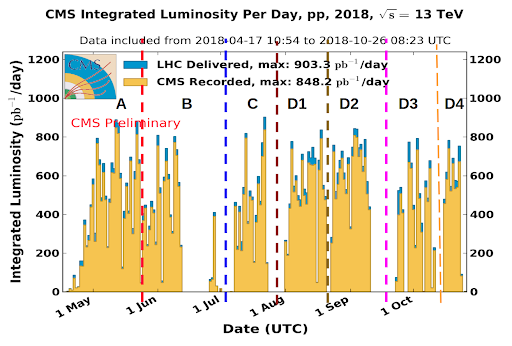
\includegraphics[width=0.9\textwidth]{ashish_thesis/period_boundary.png}
\caption[2018 CMS Luminosity Data Period]{%
   2018 luminosity data taking periods showing data taking period boundaries and vdM calibration data (1 July in period B)  \cite{CERNLumiPublicResults}.
}
\label{fig:period_bound}
\end{figure}


\begin{table}
  \begin{center}
    \caption[Run ranges for 2022 periods]{2018 luminosity data periods with run ranges.}
    \begin{tabular}{ccccc}
    \textbf{Period}   & \textbf{Run range} \\ \hline
     2018A      &        315252-316995         \\
     2018B      &        317080-319311         \\
     2018C      &        319337-320065         \\
     2018D1     &        320500-321665        \\
     2018D2     &        321710-322964         \\
     2018D3     &        323363-324420         \\
     2018D4     &        324564-325175        \\
      \end{tabular}
    %\caption[Run ranges]{2018 luminosity data periods with run ranges.}
    \label{tab:period_run_ranges}
  \end{center}
\end{table}

In the study under consideration, the datasets have been drawn from the Alignment and Calibration (AlCa) project, an integral component of the CMS experiment. The dataset selection includes two subsets: Random trigger and Zero-Bias. The Random trigger dataset comprises of data where trigger is applied on both colliding and non-colliding bunches. On the other hand, the Zero-Bias dataset encapsulates events that have passed the trigger system with no bias which means the colliding bunches are randomly triggered without the use of any CMS detector signal. The list of colliding bunches is detected by an independent system Beam Pick-up Timing system (BPTX) for Experiments. CMS software (CMSSW) version $10{\_}2{\_}2$ is used for reprocessing random trigger PCC dataset and $10{\_}6{\_}30$  \cite{CMSReleaseNotes} is used for reprocessing zero bias PCC datasets.

\begin{comment}
  
\begin{table}[htbp]
  \centering
  \begin{tabular}{@{}c@{\hspace{0.5cm}}p{6.5cm}p{6.5cm}@{}}
    \textbf{Period} & \textbf{Random Trigger Dataset} & \textbf{Zero Bias Dataset} \\
    2018A & /AlCaLumiPixels/Run2018A-\newline AlCaPCCRandom-15Apr2023\_UL2018\_\newline 315252\_316062\_PCCRandom\_-v1/ALCARECO, \newline /StreamALCALUMIPIXELSEXPRESS/\newline Run2018A-AlCaPCCRandom-Express-v1/ALCARECO & /AlCaLumiPixels/Run2018A-\newline AlCaPCCZeroBias-\newline 13Mar2023\_UL2018\_PCC-v1/ALCARECO \\
    2018B & /StreamALCALUMIPIXELSEXPRESS/\newline Run2018B-AlCaPCCRandom-Express-v1/ALCARECO & /AlCaLumiPixels/Run2018B-\newline AlCaPCCZeroBias-\newline 13Mar2023\_UL2018\_PCC-v1/ALCARECO \\
    2018C & /StreamALCALUMIPIXELSEXPRESS/\newline Run2018C-AlCaPCCRandom-Express-v1/ALCARECO & /AlCaLumiPixels/Run2018C-\newline AlCaPCCZeroBias-\newline 13Mar2023\_UL2018\_PCC-v1/ALCARECO \\
    2018D & /StreamALCALUMIPIXELSEXPRESS/\newline Run2018D-AlCaPCCRandom-Express-v1/ALCARECO & /AlCaLumiPixels/Run2018D-\newline AlCaPCCZeroBias-\newline 13Mar2023\_UL2018\_PCC-v1/ALCARECO \\
  \end{tabular}
  \caption[PCC datasets]{Datasets used for studying performance of PCC luminometer \cite{CERNDAS}}
  \label{tab:datasets}
\end{table}

\begin{table}[htbp]
  \centering
  \begin{tabular}{@{}c@{\hspace{0.5cm}}p{6.5cm}p{6.5cm}@{}}
    \textbf{Period} & \textbf{Random Trigger Dataset} & \textbf{Zero Bias Dataset} \\[1em]
    2018A & /AlCaLumiPixels/Run2018A-\newline AlCaPCCRandom-15Apr2023\_UL2018\_\newline 315252\_316062\_PCCRandom\_-v1/ALCARECO, \newline /StreamALCALUMIPIXELSEXPRESS/\newline Run2018A-AlCaPCCRandom-Express-v1/ALCARECO & /AlCaLumiPixels/Run2018A-\newline AlCaPCCZeroBias-\newline 13Mar2023\_UL2018\_PCC-v1/ALCARECO \\[1em]
    2018B & /StreamALCALUMIPIXELSEXPRESS/\newline Run2018B-AlCaPCCRandom-Express-v1/ALCARECO & /AlCaLumiPixels/Run2018B-\newline AlCaPCCZeroBias-\newline 13Mar2023\_UL2018\_PCC-v1/ALCARECO \\[1em]
    2018C & /StreamALCALUMIPIXELSEXPRESS/\newline Run2018C-AlCaPCCRandom-Express-v1/ALCARECO & /AlCaLumiPixels/Run2018C-\newline AlCaPCCZeroBias-\newline 13Mar2023\_UL2018\_PCC-v1/ALCARECO \\[1em]
    2018D & /StreamALCALUMIPIXELSEXPRESS/\newline Run2018D-AlCaPCCRandom-Express-v1/ALCARECO & /AlCaLumiPixels/Run2018D-\newline AlCaPCCZeroBias-\newline 13Mar2023\_UL2018\_PCC-v1/ALCARECO \\[1em]
  \end{tabular}
  \caption{Datasets used for studying performance of PCC luminometer}
  \label{tab:datasets}
\end{table}


\begin{table}[htbp]
  \centering
  \begin{tabular}{@{}c@{\hspace{1cm}}p{5.5cm}p{5.5cm}@{}}
    \textbf{Period} & \textbf{Random Trigger Dataset} & \textbf{Zero Bias Dataset} \\
    2018A & \begin{tabular}{@{}p{5.5cm}@{}}/AlCaLumiPixels/Run2018A-AlCaPCCRandom-15Apr2023\_UL2018\_315252\_316062\_PCCRandom\_-v1/ALCARECO, \\ /StreamALCALUMIPIXELSEXPRESS/Run2018A-AlCaPCCRandom-Express-v1/ALCARECO\end{tabular} & /AlCaLumiPixels/Run2018A-AlCaPCCZeroBias-13Mar2023\_UL2018\_PCC-v1/ALCARECO \\
    2018B & /StreamALCALUMIPIXELSEXPRESS/Run2018B-AlCaPCCRandom-Express-v1/ALCARECO & /AlCaLumiPixels/Run2018B-AlCaPCCZeroBias-13Mar2023\_UL2018\_PCC-v1/ALCARECO \\
    2018C & /StreamALCALUMIPIXELSEXPRESS/Run2018C-AlCaPCCRandom-Express-v1/ALCARECO & /AlCaLumiPixels/Run2018C-AlCaPCCZeroBias-13Mar2023\_UL2018\_PCC-v1/ALCARECO \\
    2018D & /StreamALCALUMIPIXELSEXPRESS/Run2018D-AlCaPCCRandom-Express-v1/ALCARECO & /AlCaLumiPixels/Run2018D-AlCaPCCZeroBias-13Mar2023_UL2018_PCC-v1/ALCARECO \\
  \end{tabular}
  \caption{Datasets used for studying performance of PCC luminometer}
  \label{tab:datasets}
\end{table}

\end{comment}

\begin{comment}

The calibration of luminosity measurement by the CMS experiment luminometers in the 2018 proton-proton data taking at $\sqrt{s}$ = 13 TeV \cite{CMS-PAS-LUM-18-002} was performed during LHC fill 6868 on June 30 and July 1, 2018 at $\sqrt{s}$ = 13 TeV. Zero-bias triggers on 5 bunch pairs (BCIDs 265, 865, 1780, 2192, and 3380) recorded events rate is 27.7 kHz. Trigger is applied on five colliding bunches due to limitation of the recording bandwidth. 

%\item "lsc1", was the "constant separation" scan, two beams were separated by 1.4 $\sigma$ and moved together in steps of 1 $\sigma$ across and back.
%\item "lsc2", was the "variable separation" scan method, one beam (starting with beam 1) is moved to -2.5 $\sigma$ and then a three-point scan (a "miniscan") is performed with the other beam.
%a normal VdM scan pair "norm4" and two short emittance scan pairs "emit4" and "emit5" were also performed.

%The 2018 CMS VdM scan program was conducted in two segments, interrupted by an alarm. The first segment involved six x-y scan pairs. Two were short ``emittance'' scans, named ``emit1'' and ``emit2,'' where the beams were separated by $ \(4\sigma_b\) $ over 9 steps with a 10 second integration time at each step. A standard VdM scan, named ``norm1,'' separated the beams by $\(6\sigma_b \approx 600\)~\mu m$ in 25 steps, with a 30-second duration per step. The ``offset1'' scan followed the same procedure as the standard scans but with a $\(\pm 1.5\sigma_b\)$ separation in the non-scanning direction. Lastly, two sets of ``beam imaging'' scans were conducted, where one beam remained fixed while the other was moved in 19 steps between $\(+4.5\sigma_b\)$ and $\(-4.5\sigma_b\)$, each lasting 46 seconds per step.

The 2018 CMS VdM scan program (shown in Fig. \ref{fig:vdm_prog_2018}) was conducted in two segments, interrupted by an alarm. The first segment involved six x-y scan pairs. Two were short ``emittance'' scans, named ``emit1'' and ``emit2,'' where the beams were separated by \(4\sigma_b\) over 9 steps with a 10-second integration time at each step. A standard vdM scan (described in section 3.1), named ``norm1,'' separated the beams by \(6\sigma_b \approx 600\)~$\mu$m in 25 steps, with a 30-second duration per step. The ``offset1'' scan followed the same procedure as the standard scans but with a \(\pm 1.5\sigma_b\) separation in the non-scanning direction. Lastly, two sets of ``beam imaging'' scans were conducted, where one beam remained fixed while the other was moved in 19 steps between \(+4.5\sigma_b\) and \(-4.5\sigma_b\), each lasting 46 seconds per step. The second part of the scan program was conducted in the same fill, approximately 7.5 hours later, and consisted of twelve scan pairs. This included a short emittance scan, ``emit3''; beam imaging scan pairs, ``imag2'' and ``imag3''; an offset scan pair, ``offset2''; and two standard VdM scan pairs, ``norm2'' and ``norm3''.

Beam Imaging Scans: Beam imaging scans are designed to measure the transverse profile of the beam. They involve moving one beam across the other in steps and measuring the interaction rate (or event rate) at each step. By doing this, the shape or "profile" of the beam in the transverse plane can be obtained. These scans allow for a detailed analysis of the beam shape, which is essential for understanding the beam properties. In a perfect scenario, the density distributions of protons in a bunch would factorize into separate X (horizontal) and Y (vertical) components. However, real beams can have correlations between X and Y (non-factorization). Beam imaging scans help map the 2D profile of the beam and are thus essential for diagnosing and understanding any such correlations. Knowing the 2D profile of the beams is crucial when calculating luminosity, as assumptions made about the factorization of the beam profiles feed into these calculations. By using beam imaging scans, experimenters can assess the validity of the factorization assumption or correct for any observed non-factorization.

Offset Scans: Offset scans are performed to check for systematic errors in the luminosity measurement, which may arise from various sources. They are similar to standard VdM scans but involve an intentional offset in the non-scanning direction. By comparing the results of offset scans with the results of regular scans, one can identify and correct for any systematic discrepancies that are present. Offset scans can help to assess the sensitivity of the luminosity measurement to non-factorization in the transverse plane. For example, if there are correlations between the X and Y distributions of protons (i.e., non-factorization), this could in principle affect the shape of the beam overlap region in the collision point. Offset scans, by changing the relative position of the beams, can help to assess whether such non-factorization has a significant effect on the measured luminosity.

%The second part of the scan program was conducted in the same fill, approximately 7.5 hours later, and consisted of twelve scan pairs. This included a short emittance scan, ``emit3''; beam imaging scan pairs, ``imag2'' and ``imag3''; an offset scan pair, ``offset2''; and two standard VdM scan pairs, ``norm2'' and ``norm3''.

vdM scans are typically conducted at least once a year to ensure the luminometer is correctly calibrated. Results of these scans that is the visible cross section is used to normalize the data collected by the experiments during physics run.

\begin{figure}[h]
    \centering
    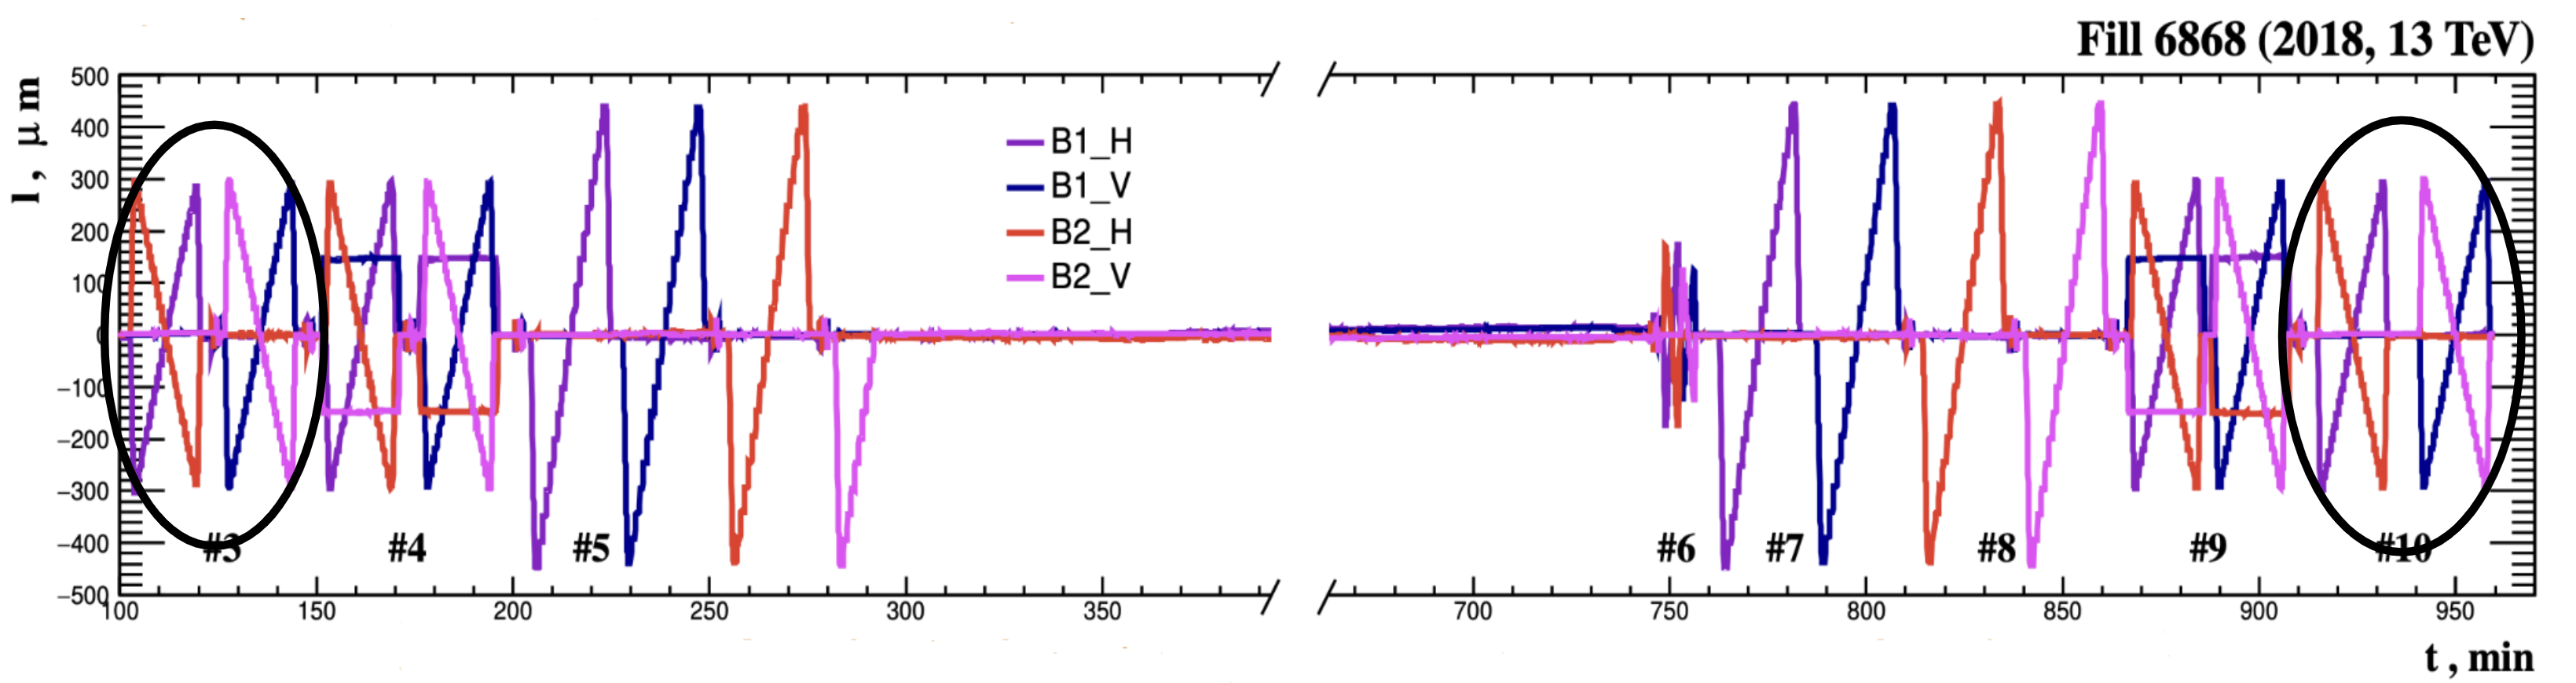
\includegraphics[width=1\textwidth]{ashish_thesis/vdm_program_2018.png}
    \caption[2018 vdM program]{Beam position along x and y is plotted as a function of time showing different types of scans. #3 and #10 are vdM scans, #4 and #9 are offset scans, #5, #7 and #8 are beam imaging scans, #6 is emittance scan.
}
    \label{fig:vdm_prog_2018}
\end{figure}

\end{comment}

%In order to measure luminosity using a pixel detector, the count of pixel clusters is studied for each module, with each module being composed of numerous pixels arranged in a grid. The number of pixel clusters recorded per unit time in each module is proportional to the instantaneous luminosity of the collider. The Pixel Cluster Counting (PCC) method is implemented by operating the pixel detector in an integrated mode. The Pixel detector is read out at a fixed interval termed a "lumi section", each lasting for 23.36 seconds.

The pixel detector records data for each bunch-crossing, though the readout rate is constrained by the trigger. During subsequent data processing,  these events are consolidated into lumi sections. During each lumi section, the number of pixel clusters produced in each module is recorded and the module weights for all pixel modules are studied to track their performance over time. This helps in identifying good and bad modules, as shown in Fig. \ref{fig:goodbadmodules}. Only pixel modules that demonstrate consistent and reliable performance throughout the entire 2018 year are considered good and included in the analysis. The pixel cluster rate, along with the visible cross section of the detector, is used to determine the instantaneous luminosity of the collider. PCC data is subsequently reprocessed. This involves the re-analysis of the data using updated or refined algorithms, calibrations, and detector conditions.

%To measure the luminosity using the pixel detector, pixel cluster count is studied for each module, where a module consists of a number of pixels arranged in a grid. The number of pixel clusters recorded in each module per unit time is proportional to the instantaneous luminosity of the collider. To implement PCC method, the pixel detector is operated in an integrated mode, where the detector is read out at a fixed time interval called a "lumi section". During each lumi section, the number of pixel clusters produced in each module is recorded, the rate of pixel clusters and visible cross section of the detector is used to determine the instantaneous luminosity of the collider. PCC data is reprocessed, a procedure that involves the re-analysis of the data using refined or updated algorithms, calibrations, or detector conditions.

The purpose of reprocessing can be multifold:

\begin{itemize}
  
\item Improved Algorithms or Calibration: As experiments progress, there can be improvements in algorithms or calibration techniques used to process the raw data. This can lead to a more accurate or efficient representation of the collected data.

\item Changes in Detector Conditions: Detector conditions might change over time due to factors like aging or upgrades. These changes can affect the interpretation of the data.

\item Discovery of Issues or Errors: Sometimes, errors or issues in the original data processing might be discovered.

\end{itemize}
  
In the context of PCC data, reprocessing can lead to a more accurate luminosity measurement, which in turn can affect the interpretation of the physics results derived from the LHC data. Random trigger PCC dataset is reprocessed with new module veto list (described in section 4.2) to obtain afterglow corrections with improved module stability selections. Zero-bias dataset is reprocessed after applying afterglow corrections using same module veto list with more stringent selections on module stability to obtain PCC luminosity.

%CMS software (CMSSW) version $10{\_}2{\_}2$ is used for reprocessing random trigger PCC dataset and $10{\_}6{\_}30$  \cite{CMSReleaseNotes} is used for reprocessing zero bias PCC datasets. %Datasets can be obtained by applying triggers on all bunches (colliding and non colliding) and only on colliding bunches to get random trigger and zero bias data respectively as described in previous section.
%Random trigger PCC dataset is reprocessed with new module veto list (described in section 4.2) to obtain afterglow corrections with improved module stability selections. Zero-bias dataset is reprocessed after applying afterglow corrections using same module veto list with more stringent selections on module stability to obtain PCC luminosity. 
%To ensure accurate luminosity measurements, it is necessary to correct for various effects, such as detector inefficiencies and pileup (the presence of additional proton-proton collisions in the same bunch crossing). This is achieved through careful calibration of the detector and by using dedicated algorithms to estimate the contribution of pileup to the observed pixel cluster counts.

\begin{comment}

\begin{table}
  \begin{center}
    \begin{tabular}{ccccc}  
    \textbf{Period}   & \textbf{Run range} \\ \hline
     2018A      &        315252-316995         \\ 
     2018B      &        317080-319311         \\ 
     2018C      &        319337-320065         \\ 
     2018D1     &        320500-321665        \\ 
     2018D2     &        321710-322964         \\ 
     2018D3     &        323363-324420         \\ 
     2018D4     &        324564-325175        \\ 
      \end{tabular}
    \caption{2018 luminosity data periods with run ranges.}
    \label{tab:period run ranges}
  \end{center}
\end{table}

\section{Software tools}

%CERN ROOT is a software framework commonly used in particle physics to analyze large datasets generated by particle detectors such as the CMS experiment at CERN. One of the important measurements performed at CMS is the determination of the instantaneous luminosity, which is a measure of the rate at which particles are colliding in the detector. To measure the luminosity at CMS, the detector records signals from various sub-detectors, such as the silicon tracker and the calorimeters, which are used to reconstruct the tracks and energy deposits of particles produced in the collisions. These signals are then processed using the CERN ROOT framework to extract relevant information such as the number of collisions per second and the total integrated luminosity over a given period of time.The CERN ROOT framework is used to analyze the data from van der Meer scans and extract the luminosity calibration factors needed to convert the collision rates into actual luminosity measurements. To extract Pixel Cluster Counting (PCC) datasets from the CMS Data Aggregation Service (DAS) using a shell script, we can use the dasgoclient command-line tool. For example, following command can copy names of all root files into a text file.
 
%\begin{verbatim}
 % dasgoclient -query="file dataset=/AlCaLumiPixels/Run2018A-AlCaPCCZeroBias- 27Oct2022_UL2018_PCC-v1/ALCARECO instance=prod/global | grep file.name | grep  '.root'" > Run2018A.txt   
%\end{verbatim}

%\begin{itemize}
    
%\item  In the CMS experiment at CERN, luminosity measurements using the Pixel Cluster Counting (PCC) method are typically performed using the CMSSW framework. The luminosity module and configuration files used in CMSSW to perform PCC luminosity measurements can be generated using C++ code and Python scripts. 

%\item  HTCondor is used to process PCC datasets, is a high-throughput computing (HTC) system that can be used to submits jobs for each run to efficiently manage large-scale data processing tasks, such as those required in the analysis of data from high-energy physics experiments. HTCondor provides a framework for distributing and managing the processing of this data across a large number of computing nodes. This allows the luminosity measurement to be performed more quickly and efficiently than would be possible using a traditional computing approach. Specifically, 

%\item HTCondor is used to manage the processing of so-called "luminosity blocks" of data, which correspond to periods of time during which the accelerator was operating at a certain luminosity. These blocks can contain many terabytes of data, and processing them requires significant computing resources. With HTCondor, the processing of these blocks can be distributed across a large number of computing nodes, allowing the analysis to be performed in parallel. Additionally, HTCondor provides features for managing the scheduling of jobs and ensuring that data is transferred between nodes efficiently, which is critical for achieving high throughput in the analysis.

%\end{itemize}

\begin{itemize}

\item CMSSW: The CMS Software (CMSSW) is a comprehensive software framework developed for the Compact Muon Solenoid (CMS) experiment at the Large Hadron Collider (LHC) at CERN. CMSSW is used for the simulation, processing, and analysis of data collected by the CMS detector. It is designed to handle various tasks, from the generation of simulated events to the reconstruction of raw detector data, calibration, and high-level analysis. CMSSW is composed of several interconnected components and follows a modular architecture to promote flexibility, reusability, and maintainability. Some key aspects of CMSSW include, Event Data Model (EDM): The EDM serves as the foundation of CMSSW, defining the structure and organization of data objects, such as particle candidates, detector hits, and reconstructed vertices. It is designed to handle the storage, retrieval, and manipulation of these objects efficiently. The CMSSW framework is responsible for the management of software modules, the flow of data between modules, and the execution of the necessary tasks. It also handles the scheduling of tasks and the parallelization of processes, enabling efficient use of computing resources. Modules: CMSSW is built upon a collection of software modules, each responsible for a specific task, such as event generation, detector simulation, reconstruction, or analysis. These modules can be combined and customized to create a complete processing chain for a given use case. The software includes a detailed description of the CMS detector geometry, material properties, and readout electronics. This information is used during the simulation and reconstruction processes to accurately model the detector's response to particles. 
Simulation: CMSSW integrates several external tools and libraries, such as the GEANT4 toolkit, to simulate the passage of particles through the CMS detector. This includes the interactions of particles with the detector material, the production of secondary particles, and the generation of detector signals. Reconstruction: The reconstruction algorithms in CMSSW process the raw detector data, converting it into meaningful physics objects, such as tracks, calorimeter clusters, and particle candidates. These algorithms use a variety of techniques, including pattern recognition, clustering, and fitting, to extract the relevant information from the detector signals. CMSSW includes tools for the calibration of detector components and the alignment of the detector geometry. These tasks are crucial for ensuring the accurate reconstruction of physics objects and the extraction of meaningful results from the data. Analysis: The software provides a rich set of high-level analysis tools and libraries, enabling researchers to perform a wide range of physics analyses, from searches for new particles to precision measurements of Standard Model processes. Data storage and management: CMSSW uses the ROOT data format for the storage and management of data objects. ROOT is a powerful and flexible data storage and processing framework developed at CERN, which provides efficient data handling, advanced statistical analysis tools, and extensive data visualization capabilities \cite{CMSWorkBook}.

\item Conditions Database (CondDB): The Conditions Database (CondDB) is a centralized data storage and management system used in high-energy physics experiments, such as the Compact Muon Solenoid (CMS) at the Large Hadron Collider (LHC) at CERN. The primary purpose of CondDB is to store non-event-related data, known as "conditions data," which is essential for the proper interpretation and analysis of the experimental data. Conditions data includes information on the detector's configuration, calibration constants, alignment parameters, and other time-dependent data that characterize the performance and status of the detector and its components. Since the conditions data is critical for accurate data processing and analysis, it must be readily accessible and easily managed. CondDB provides a central repository for storing conditions data from various sources, such as detector control systems, calibration measurements, and offline analyses. This centralization simplifies data management and ensures that all data processing tasks have access to the same, consistent information. Time-dependent data management: The database is designed to handle time-dependent data efficiently. Each data record stored in CondDB is associated with a specific time interval, known as the "IOV" (Interval of Validity). This enables the retrieval of the correct conditions data corresponding to a specific data-taking period. Data versioning: CondDB supports versioning of the conditions data, allowing researchers to track changes and updates to the data over time. This feature ensures reproducibility of results and facilitates comparisons between different data processing and analysis workflows. Access control: The database provides fine-grained access control mechanisms, enabling authorized users to read, write, and modify conditions data. This ensures the integrity of the data and prevents unauthorized modifications. CondDB is designed to handle the large volume of conditions data generated by high-energy physics experiments, with efficient data storage and retrieval mechanisms. The database is built on robust and scalable technologies, such as relational databases (e.g., Oracle, MySQL, or PostgreSQL), to ensure high performance and reliability. Integration with data processing frameworks: The Conditions Database is designed to integrate seamlessly with data processing and analysis frameworks, such as the CMS Software (CMSSW). This integration allows for the automatic retrieval and usage of conditions data during the data processing workflow, ensuring the correct data is used at each step of the process.

\item HTCondor: HTCondor is a specialized workload management system designed for distributed computing environments. Developed at the University of Wisconsin-Madison, HTCondor is an open-source system that facilitates the efficient utilization of computing resources by managing and scheduling compute jobs across a network of computers. It is widely used in various scientific domains, including high-energy physics, bioinformatics, and computer science, to handle large-scale computational tasks. HTCondor is designed to discover, monitor, and manage a heterogeneous collection of computing resources, including desktop computers, dedicated clusters, and cloud computing resources. It can efficiently allocate jobs to resources based on the requirements of the jobs and the availability of the resources. HTCondor provides a sophisticated job scheduling system, which prioritizes and assigns jobs to appropriate resources based on various criteria, such as resource availability, job requirements, and user-defined policies. The scheduler supports various scheduling strategies, including fair-sharing, priority-based, and opportunistic scheduling. HTCondor is designed to be fault-tolerant and can automatically recover from failures or interruptions in the computing environment. In case a job fails to complete due to a system crash or network disconnection, HTCondor can reschedule the job to another available resource, ensuring that the job eventually completes. Data management: HTCondor provides built-in data management capabilities, allowing users to transfer input and output files between the submitting machine and the executing machines. This feature simplifies data handling in distributed computing environments and ensures that jobs have access to the required data. HTCondor provides a range of security mechanisms to protect the integrity and confidentiality of both the jobs and the computing resources. These mechanisms include authentication, authorization, data encryption, and sandboxing, which prevent unauthorized access and tampering. HTCondor enables users to monitor the progress of their jobs, providing information on job status, resource usage, and performance. Users can also control their jobs by pausing, resuming, or canceling them as needed. Interoperability and extensibility: HTCondor is designed to interoperate with other computing systems and can be easily integrated into existing workflows. It supports various job submission languages, such as the Job Submission Description Language (JSDL) and the ClassAd language, and can be extended with custom plugins and scripts. HTCondor is compatible with a wide range of operating systems, including Linux, macOS, and Windows, enabling users to harness the full potential of their computing resources, regardless of the underlying platform.

\item CMS Data Aggregation System (DAS): The CMS Data Aggregation System (DAS) is a data management tool designed for the Compact Muon Solenoid (CMS) experiment at the Large Hadron Collider (LHC) at CERN. It serves as a centralized query system that simplifies the process of locating and accessing various types of CMS data and metadata. DAS aggregates information from multiple data services and presents it in a unified manner, enabling researchers to easily search for and retrieve the data they need for their analyses. DAS provides a unified query language that allows users to perform searches across different data services using a single, consistent syntax. This simplifies the process of data discovery and reduces the learning curve associated with using multiple data services. DAS is designed to aggregate data from various data services within the CMS experiment, including data storage systems, data catalogs, and data processing services. By consolidating this information, DAS enables researchers to easily search for and access the data they need, without having to interact with multiple data services individually. Data caching: To improve performance and reduce the load on the underlying data services, DAS employs a caching mechanism that temporarily stores the results of previous queries. This allows DAS to quickly return results for frequently requested queries, without having to query the data services each time. DAS can merge data from multiple sources, providing users with a consolidated view of the information. This feature simplifies data analysis by eliminating the need for researchers to manually merge data from different sources. DAS supports data transformation operations, such as filtering, sorting, and aggregation, allowing users to customize the output of their queries to meet their specific needs. This feature helps researchers focus on the most relevant information and reduces the amount of data they need to process. DAS is designed to be extensible, enabling the integration of additional data services as needed. This allows DAS to adapt to the evolving needs of the CMS experiment and continue to provide a unified interface for data discovery and access. DAS offers a web-based user interface that allows users to submit queries and view the results using a standard web browser. This makes it easy for researchers to access and use the system, regardless of their location or computing environment. API access: In addition to the web-based user interface, DAS provides an Application Programming Interface (API) that allows users to programmatically submit queries and retrieve results. This enables the integration of DAS with other software tools and workflows used by the CMS experiment.

\item Brilcalc: The brilcalc tool is a software package designed to calculate and analyze luminosity data for the Compact Muon Solenoid (CMS) experiment at the Large Hadron Collider (LHC) at CERN. Luminosity is a crucial parameter in high-energy physics experiments like CMS, as it measures the rate of collisions in a particle accelerator and directly affects the statistical significance of experimental results. Brilcalc serves as a command-line interface (CLI) tool, which allows users to extract, manipulate, and visualize luminosity data from the CMS experiment. It is built upon the BRIL (Beam Radiation Instrumentation and Luminosity) project, which is responsible for the development and maintenance of beam monitoring and luminosity measurement systems at the CMS experiment. Users can extract luminosity data for a specific data-taking period or data range from the CMS database. The data can be filtered by various criteria, such as run number, fill number, and data-taking conditions. Data manipulation: The tool offers the capability to process and manipulate the extracted luminosity data. Users can perform operations such as unit conversion, data scaling, and data normalization to make the data suitable for further analysis. Brilcalc allows users to perform basic statistical analyses on the luminosity data, such as calculating integrated luminosity, average luminosity, and instantaneous luminosity. These analyses help physicists understand the performance of the CMS detector and plan future data-taking strategies. The tool can generate plots and graphs to visualize the luminosity data, making it easier for researchers to interpret the results and identify trends or anomalies. Brilcalc is designed to be extensible, allowing users to develop custom plugins and scripts for advanced data analysis and visualization tasks \cite{CMSLuminosityCalculationGuide}.

\item CERN ROOT: The ROOT data analysis framework, developed by CERN, is widely used in high-energy physics experiments, including CMS. ROOT offers a rich set of tools for data processing, statistical analysis, and visualization. In the context of PCC luminosity measurement, ROOT is employed to analyze and process the output data from CMSSW, perform statistical analyses, and generate plots for data visualization \cite{ROOT}.

\item Shell/Bash Scripting: Shell and bash scripting are widely used in high-energy physics research to automate repetitive tasks and manage workflows. These scripting languages offer flexibility and portability, allowing researchers to create custom scripts tailored to their specific needs. In the context of PCC luminosity measurement, shell/bash scripts are employed to streamline data processing, automate job submission to HTCondor, and manage the overall workflow, enhancing productivity and reducing the chances of human error.

\item DASgoclient: The DASgoclient is a command-line interface for the CMS Data Aggregation System (DAS). It offers researchers an alternative method for accessing various CMS data services without using the web-based DAS interface. The DASgoclient allows users to query and retrieve data in a more scriptable and automated manner, making it an essential tool for managing datasets and streamlining the data retrieval process for PCC luminosity measurement.

\end{itemize}

%\begin{figure}[!htp]
%\centering
%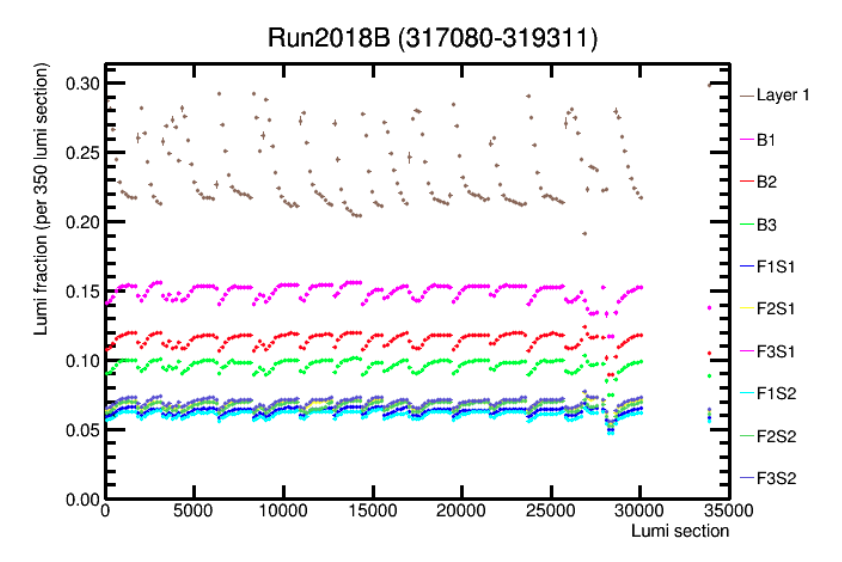
\includegraphics[width=0.8\textwidth]{ashish_thesis/pcc_stability_begin.png}
%\caption{%                                                                                                                                                                                          
 %  Luminosity fraction of pixel detector for various layer and disks as a function of lumi section after removing low statistics lumi section.
%}
%\label{fig:PCC_stab_begin}
%\end{figure}

%\begin{figure}[!htp]
%\centering
%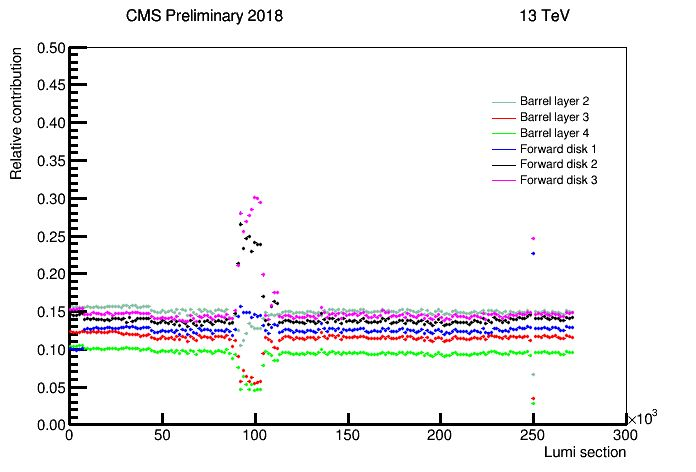
\includegraphics[width=0.8\textwidth]{ashish_thesis/pixel_layer_disk_noveto_noselection.png}
%\caption{%                                                                                                                                                                                                            
 %  Luminosity fraction of pixel detector for various layer and disks as a function of lumi section after removing low statistics lumi section.
%}
%\label{fig:PCC_stab_begin}
%\end{figure}


%\begin{figure}[!htp]
%\centering
%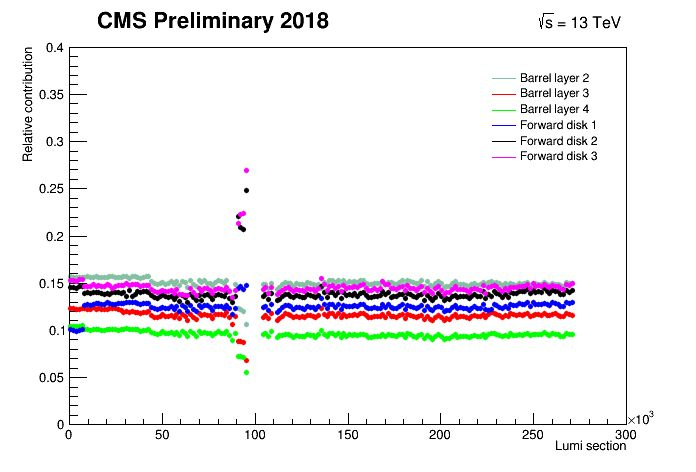
\includegraphics[width=0.8\textwidth]{ashish_thesis/pixel_layer_disk_noveto.png}
%\caption{%                                                                                                                                                                
 %  Luminosity fraction of pixel detector for various layer and disks as a function of lumi section after removing low statistics lumi section.
%}
%\label{fig:PCC_stab_begin}
%\end{figure}



%\begin{figure}[!htp]
%\centering
%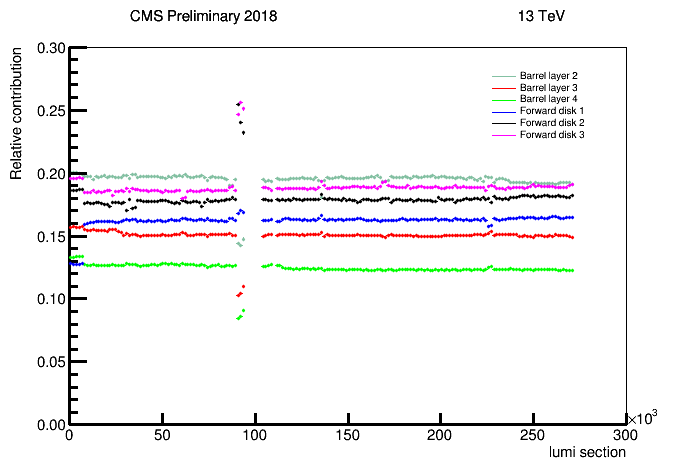
\includegraphics[width=0.8\textwidth]{ashish_thesis/pcc_frac_L0_veto.png}
%\caption{%                                                                                                                                                                           
 %  Luminosity fraction of pixel detector for various layer and disks as a function of lumi section after removing low statistics lumi section.
%}
%\label{fig:PCC_stab_L0_veto}
%\end{figure}


%\begin{figure}[!htp]
%\centering
%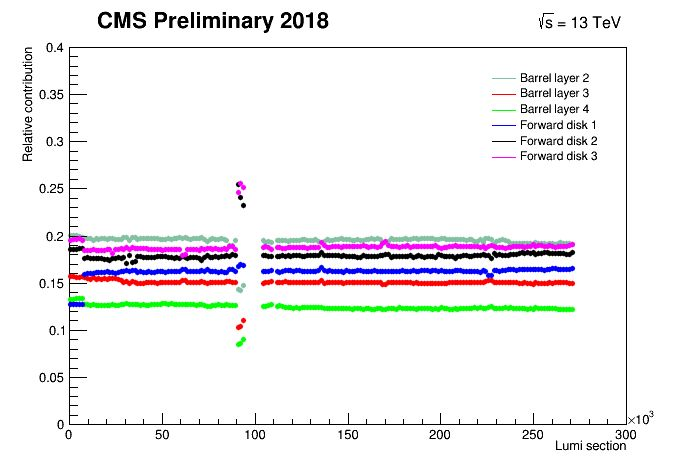
\includegraphics[width=0.8\textwidth]{ashish_thesis/pixel_layer_disk_B0_veto.png}
%\caption{%                                                                                                                                                                           
 %  Luminosity fraction of pixel detector for various layer and disks as a function of lumi section after removing low statistics lumi section and all modules in Layer 1.
%}
%\label{fig:PCC_stab_L0_veto}
%\end{figure}

\end{comment}


\section{Detector module selection}

The goal of minimizing instabilities in PCC luminosity measurement is to ensure precise and consistent results. To achieve this, a pixel module veto list is created for each period to keep track of  bad modules. The stability of each module is determined based on the change in the ratio of module PCC and total PCC, referred to as the module weight. %as shown in Fig. \ref{fig:mod_weight}.

%\begin{itemize}

%\item Lumi section duration: The data collected for luminosity measurements are divided into lumi sections, each lasting for 23.36 seconds.

%\item Analyzing module weights: During each lumi section, the module weights for all pixel modules are studied to track their performance over time. This helps in identifying good and bad modules, as shown in Fig. \ref{fig:goodbadmodules}.

%\item Pixel detector composition: The pixel detector used for the 2018 luminosity measurement comprises two main components - the BPIX (barrel pixel detector) with 4 barrel layers, and the FPIX (forward pixel detector) with three forward disks. These two components consist of 1184 and 672 pixel modules, respectively.

%\item Selection criteria: Only pixel modules that demonstrate consistent and reliable performance throughout the entire 2018 year are considered good and included in the analysis. %Modules that do not meet these criteria are classified as bad and excluded from the luminosity measurement.

%\end{itemize}

By carefully analyzing the module weights and excluding the bad modules from the analysis, the instabilities in PCC luminosity measurement can be minimized. This process ensures that the data used for luminosity measurement is of high quality and can produce precise results.

%To minimize instabilities in PCC luminosity measurement, pixel module vetolist is created for each run period. Module stability is based on change in the ratio of module PCC and total PCC which is defined as module weight. Change in module weights with lumi section (23.36s) is studied for all modules and used to select good and bad modules as shown in Fig. \ref{fig:goodbadmodules}. Pixel detector used for 2018 luminosity measurement consists of 4 barrel layers (BPIX) and three forward disks (FPIX) including 1184 and 672 pixel modules respectively. Only pixel modules that are found to show good performance during the entire 2018 year are selected. 

%\begin{figure}[!htp]
%\centering
%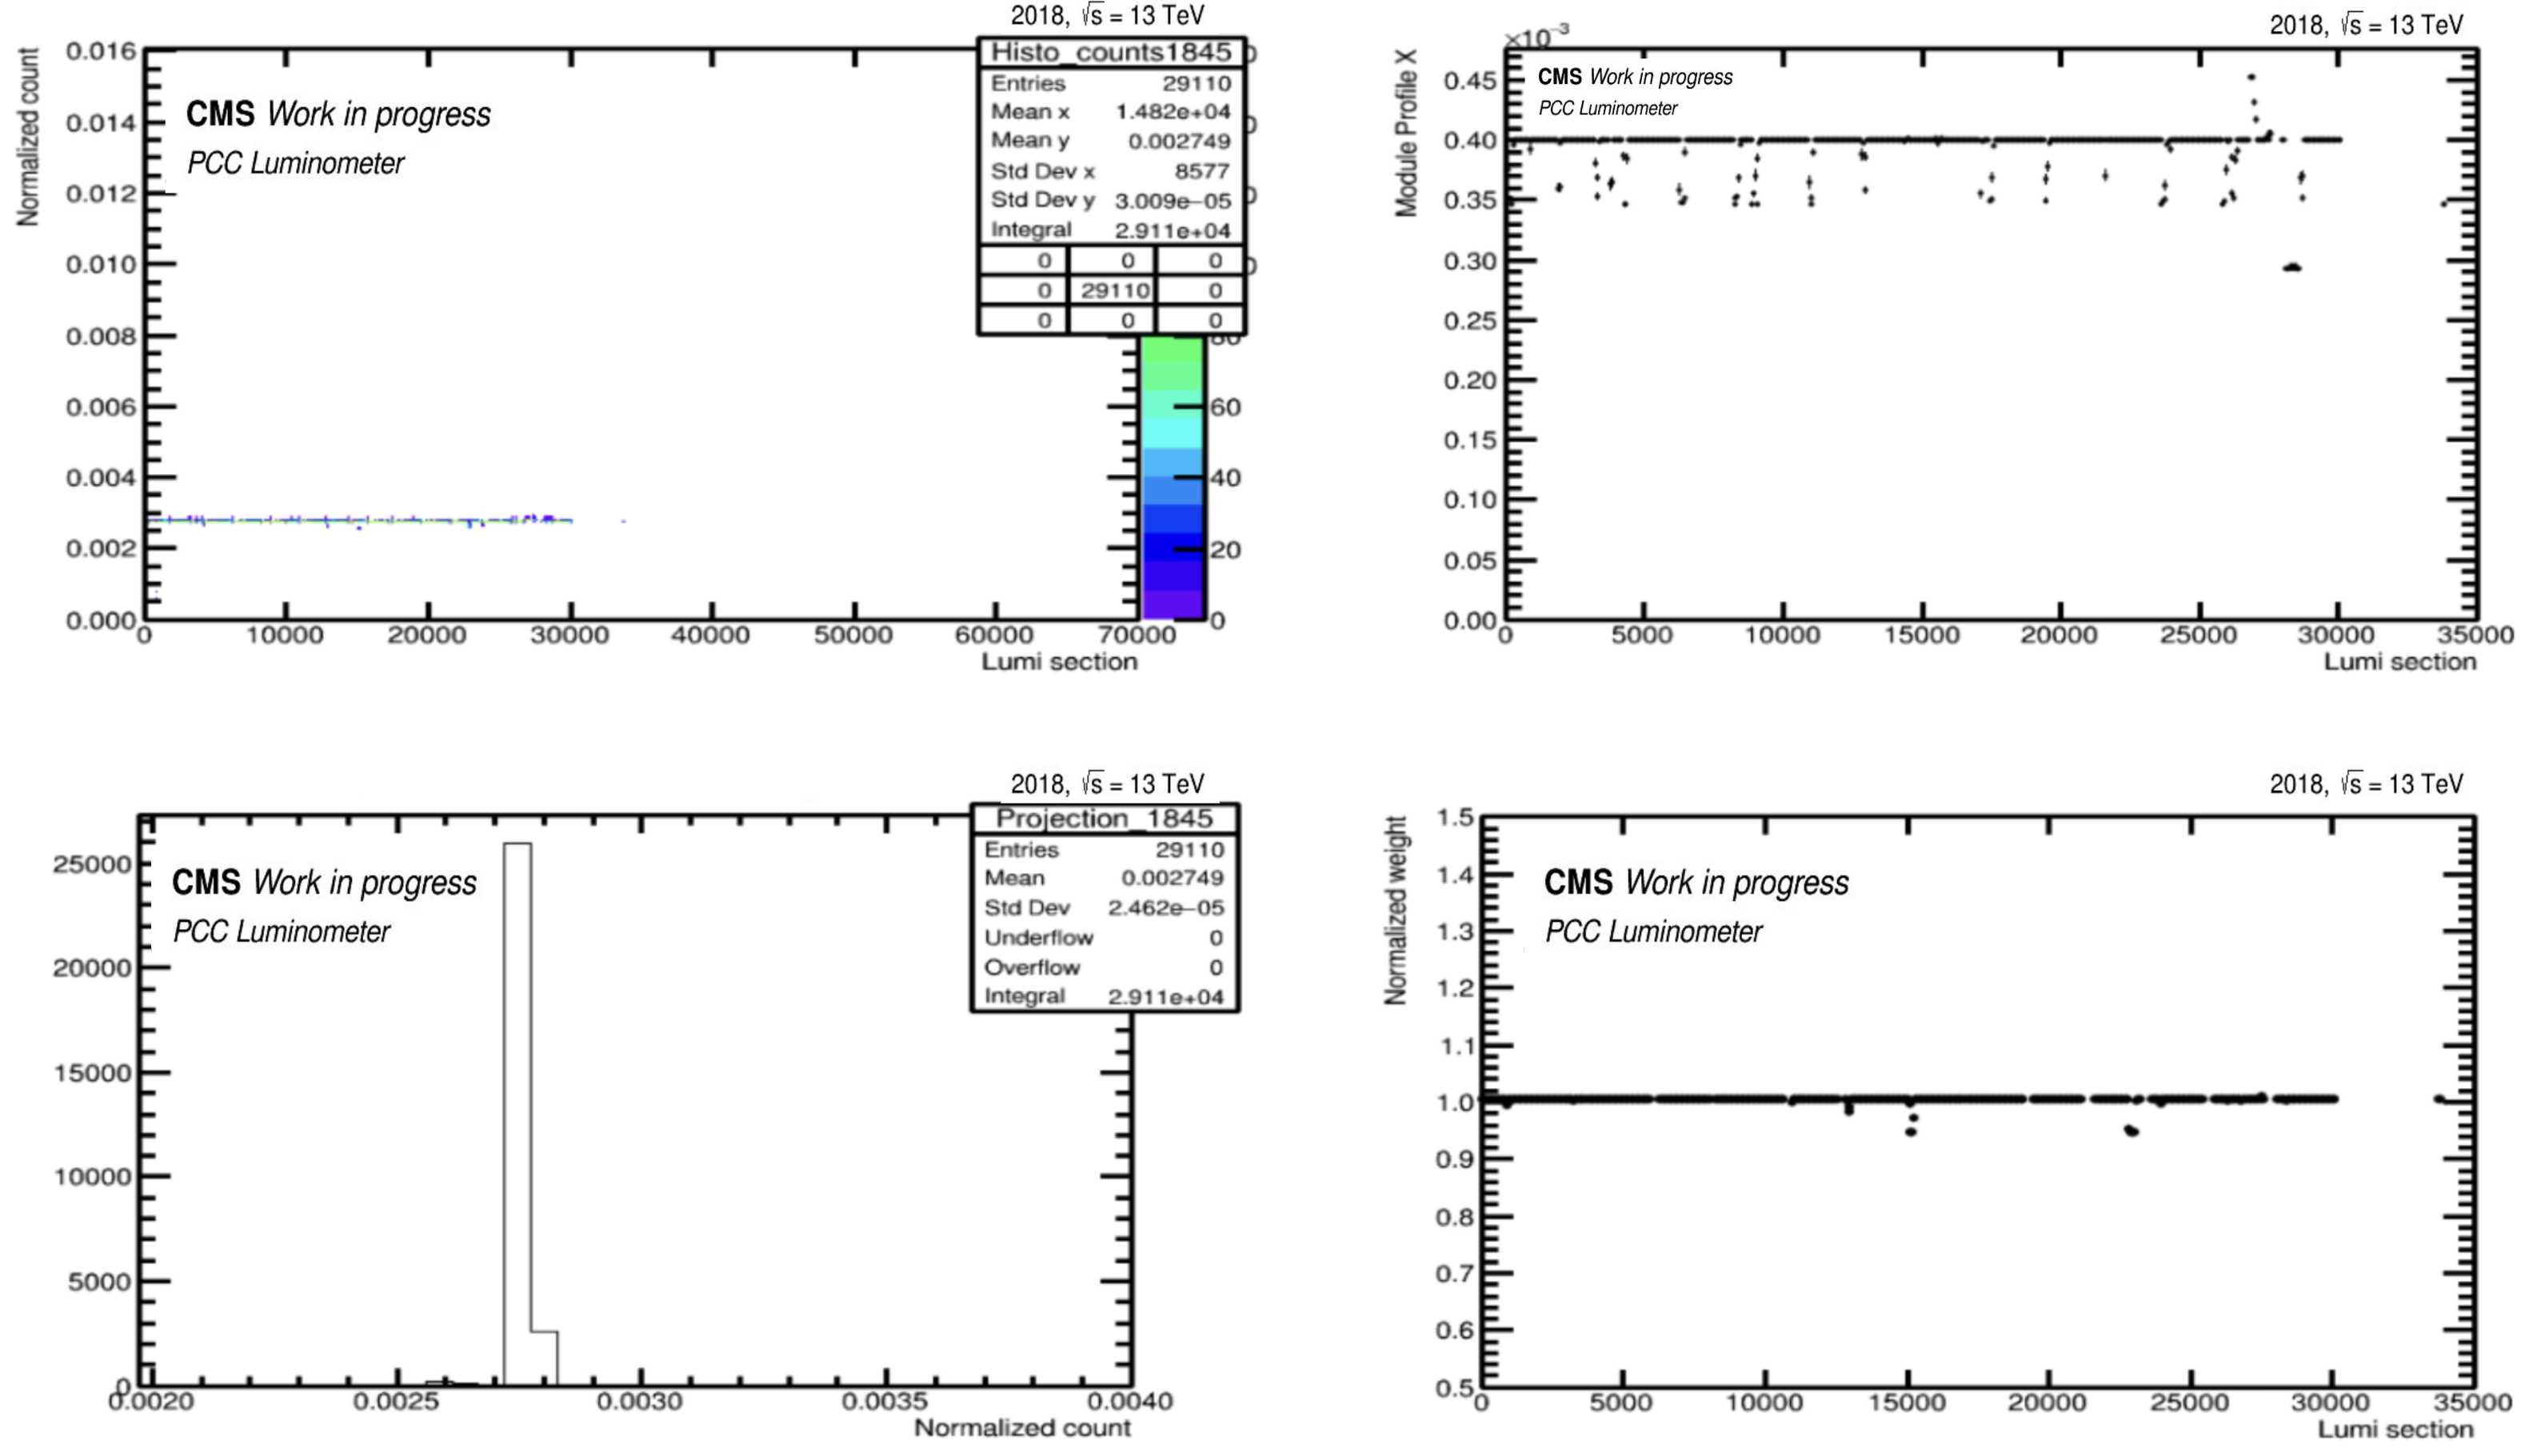
\includegraphics[width=1\textwidth]{ashish_thesis/Module_weight_2.png}
%\caption[Module Weight]{%
 %  Method to obtain module weights as a function of lumi section for categorizing good and bad modules. X profile of TH2F histogram (module PCC/total PCC per lumi section) is obtained. X profile is then filled in a TGraph after removing points with error $>$ 0.05. TGraph is normalized with the mean of Y projection of TH2F histogram to obtain module stability profile.
%}
%\label{fig:mod_weight}
%\end{figure}


\begin{figure}[!htp]
\centering
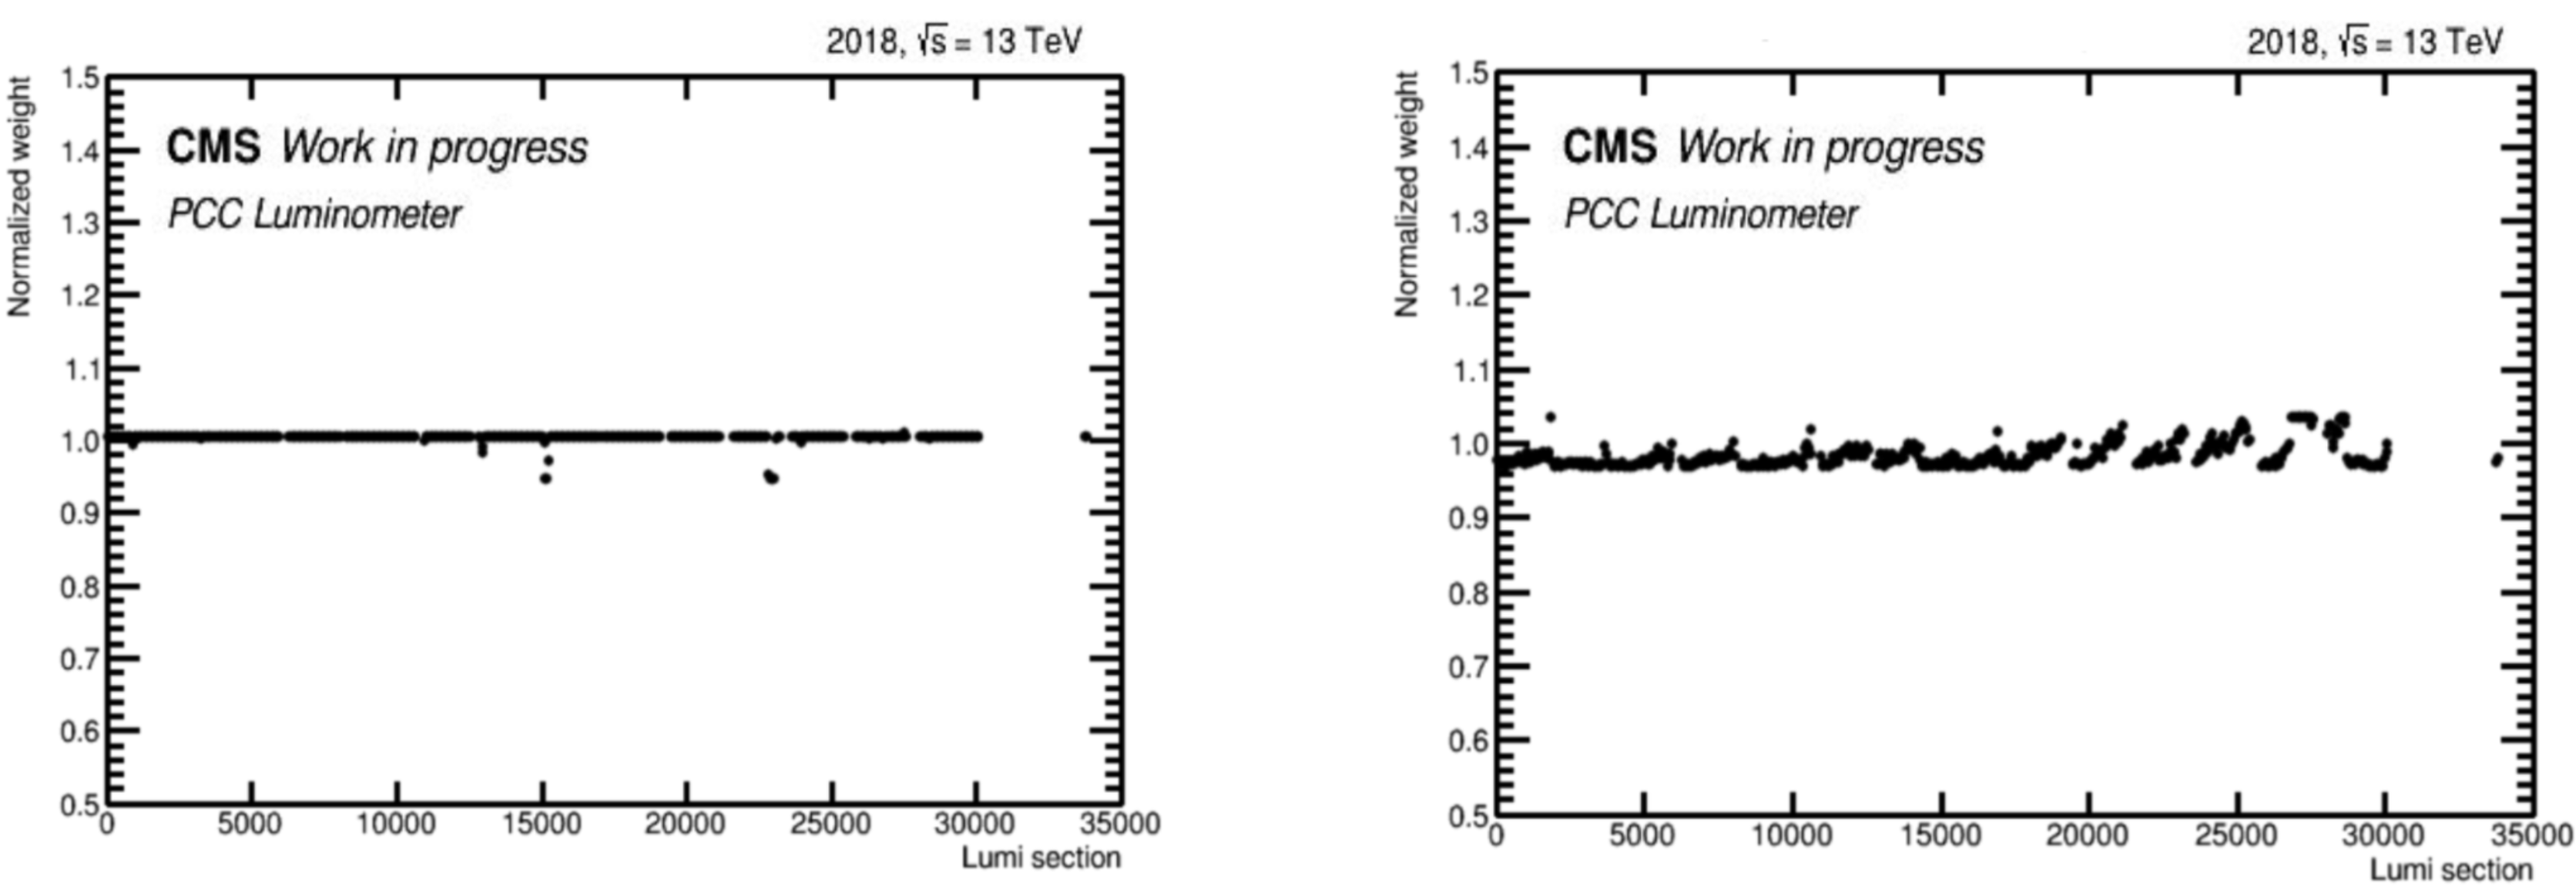
\includegraphics[width=1\textwidth]{ashish_thesis/good_bad_modules_1.png}
\caption[Good/Bad Module Weights]{%
   Change in normalized module weight with time. Modules showing significant change in module weight (shown in right figure) over time having large RMS/mean values are used to make module veto list.
}
\label{fig:goodbadmodules}
\end{figure}

The module veto list is a list of detector modules that are excluded from the analysis of data due to their known or suspected high rate of background events or other issues that could affect the accuracy of the measurement. The following factors lead to unstable modules: 

\begin{itemize}

\item Radiation damage: The harsh radiation environment in the LHC can cause damage to the silicon pixel sensors over time, leading to increased leakage currents, noise, or reduced charge collection efficiency.

\item Manufacturing defects: Defects in the silicon material or issues during the manufacturing process can result in poorly performing pixel modules. These defects may not be immediately evident but can become more pronounced overtime.

\item Electronic noise: Noisy electronic components or crosstalk between channels can lead to an increased number of false signals or noise in the pixel module data.

\item Temperature variations: Temperature fluctuations can affect the performance of the pixel modules, leading to changes in their noise levels, gain, or charge collection efficiency.

\item High voltage issues: Problems with the high voltage supply to the pixel modules can result in unstable operation, leading to erratic behavior or complete module failure.

\item Partial module failure: A pixel module may suffer from partial failure, with some pixels or readout channels not functioning properly. This can lead to an increased number of dead or noisy pixels in the module.

\item Readout or data acquisition issues: Errors in the readout electronics or data acquisition system can lead to data corruption or loss, affecting the performance of the pixel modules.

\item Calibration issues: Inaccurate or outdated calibration parameters can result in incorrect measurements, leading to the appearance of abnormal behavior in the pixel module data.

\item Firmware or software issues: Bugs in the firmware or software responsible for controlling and reading out the pixel modules can lead to abnormal behavior or incorrect measurements.

\item Mechanical or alignment issues: Mechanical stresses or misalignments during the installation or operation of the pixel detector can affect the performance of the pixel modules or cause them to fail.

\item Contamination or environmental factors: Contamination of the pixel modules by dust, moisture, or other substances can affect their performance or cause them to fail. Similarly, external environmental factors, such as magnetic fields or vibrations, can impact the operation of the pixel modules.

\end{itemize}

%The inclusion of certain modules in the veto list is based on a careful analysis of the detector performance and the expected background rates in a given experiment. By excluding modules with high background rates or other issues, the analysis can be improved and the accuracy of the measurement can be increased.

Module veto list consisting of bad modules is first created for period B, vdM Fill and then for other periods A, C, D1, D2, D3 and D4 as follows, 

Run 2018B and vdM Fill:
\begin{itemize}

\item Poor statistics lumi sections are removed by applying selection on total PCC. %Fig. \ref{fig:PCC_cut}. % and \ref{fig:f_it}.

\item All barrel layer 1 modules are removed as these modules are significantly affected by dynamic inefficiency effects, where the hit efficiency decreases at higher instantaneous luminosity due to the readout chip not being able to process all of the hits.
  
\item A loose selection of 7\% based on RMS/mean of module weight profile is applied where mean and RMS values are obtained from y projection of module weight profile. Modules with significantly large RMS/mean are removed with this loose selection as shown in Fig. \ref{fig:outliermodules}. 

\item Module stability is re-evaluated based on RMS/mean values using an iterative method where in each step, appropriate selections are applied to remove bad modules (shown in Fig. \ref{fig:sec_it_cut}) until stable luminosity is attained.                                                      
\end{itemize}

Run 2018A, C and D:                                                                      
\begin{itemize}  

\item Period B module vetolist is applied to these periods to determine remaining bad modules.

\item same procedure is used as period B. 

\item module weight comparisons between period B and these periods is done and modules with more than 3 sigma change in module weights are removed as shown in %Fig. \ref{fig:mod_w_com} and
  Fig \ref{fig:mod_w_com_1}.                                                                              
\end{itemize}

%\begin{figure}[t]
%\centering
%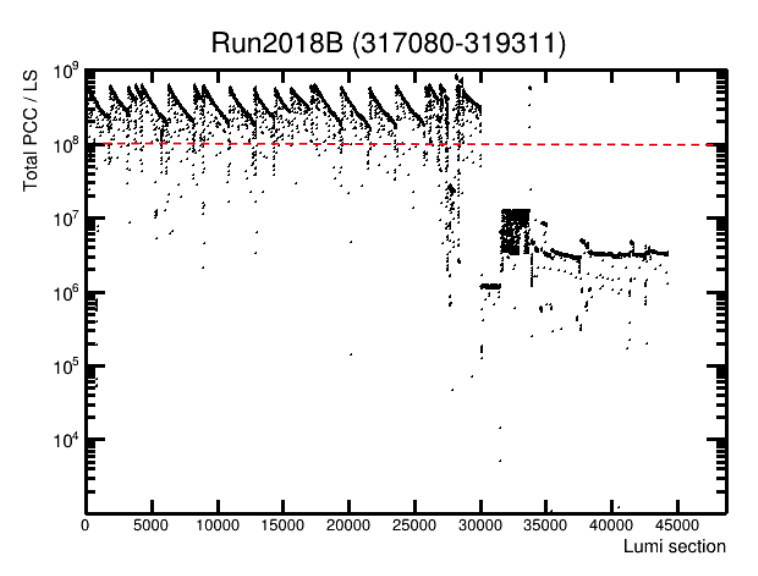
\includegraphics[width=0.7\textwidth]{ashish_thesis/Run2018B_totalPCC_cut.png}
%\caption[Low Statistics Lumi section Filtering]{%
% Total PCC as a function of lumi section for period 2018B. Appropriate selection on total PCC shown by the red line is applied to remove low statistics lumi sections.
%}
%\label{fig:PCC_cut}
%\end{figure}

%\begin{figure}[!htp]
%\centering
%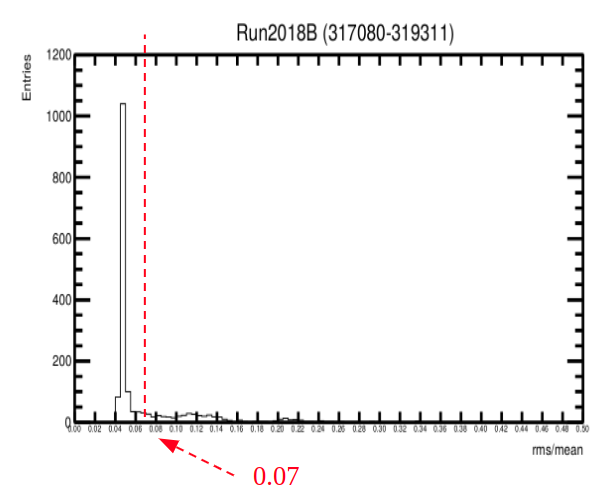
\includegraphics[width=0.7\textwidth]{ashish_thesis/first_iteration.png}
%\caption{%
%   A loose cut of 7\% is applied on rms/mean values of module stability profile to remove outlier modules.
%}
%\label{fig:f_it}
%\end{figure}

\begin{figure}[!htp]
\centering
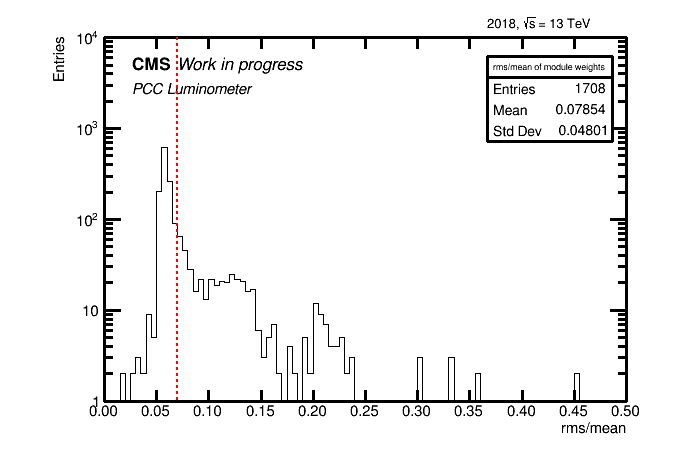
\includegraphics[width=0.8\textwidth]{ashish_thesis/cut_selection_1.png}
\caption[First Iteration For Outlier Module Removal]{%
   A loose selection of 7\% is applied to remove bad modules. Appropriate selections are applied in each iterative step to remove other bad modules.
}
\label{fig:outliermodules}
\end{figure}

\begin{figure}[!htp]
    \centering
    %\begin{minipage}{0.45\textwidth}
        \centering
        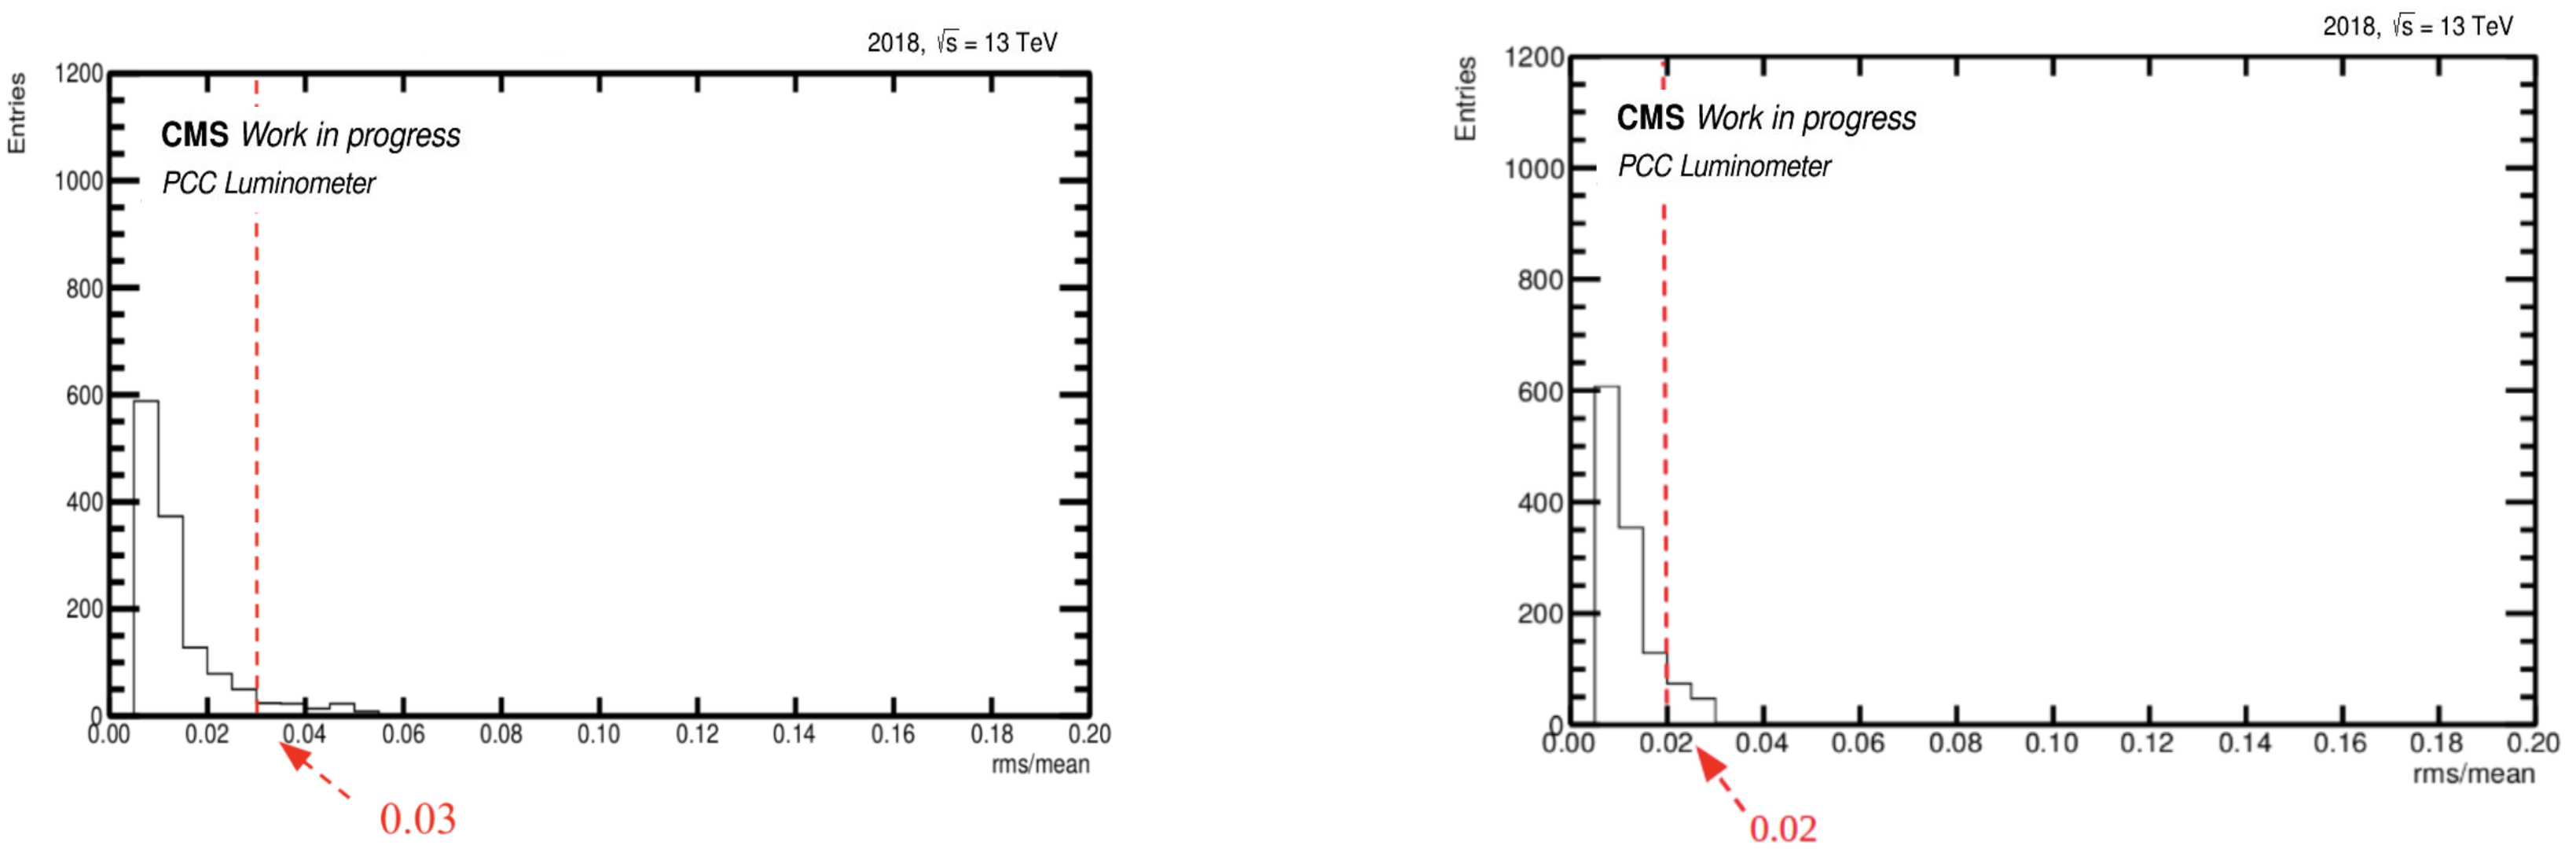
\includegraphics[width=1.0\linewidth]{ashish_thesis/3percent_cut_1.png}
    %\end{minipage}
    %\hfill
    %\begin{minipage}{0.45\textwidth}
     %   \centering
      %  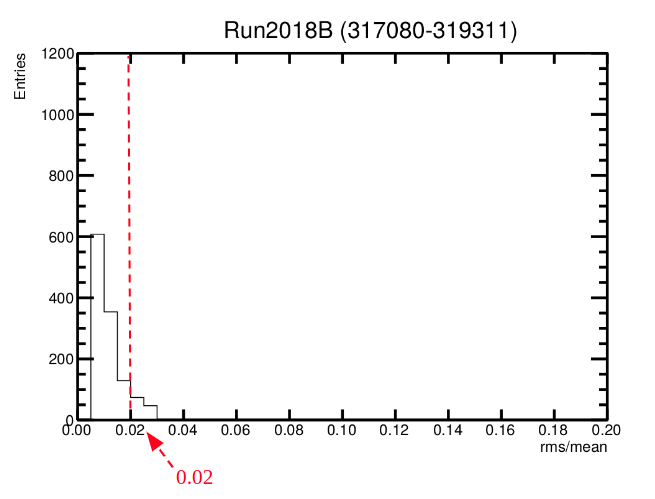
\includegraphics[width=1.0\linewidth]{ashish_thesis/second_iteration_cut.png}
    %\end{minipage}
    
    \caption[Second and Final Iteration For Outlier Module Removal]{%
        Left: Second iteration on RMS/mean of 3\% is applied to remove more bad modules. 
        Right: Final iteration on RMS/mean of 2\% is applied to obtain module veto list for each period.
    }
    \label{fig:sec_it_cut}
\end{figure}








\begin{comment}

\begin{figure}[!htp]
\centering
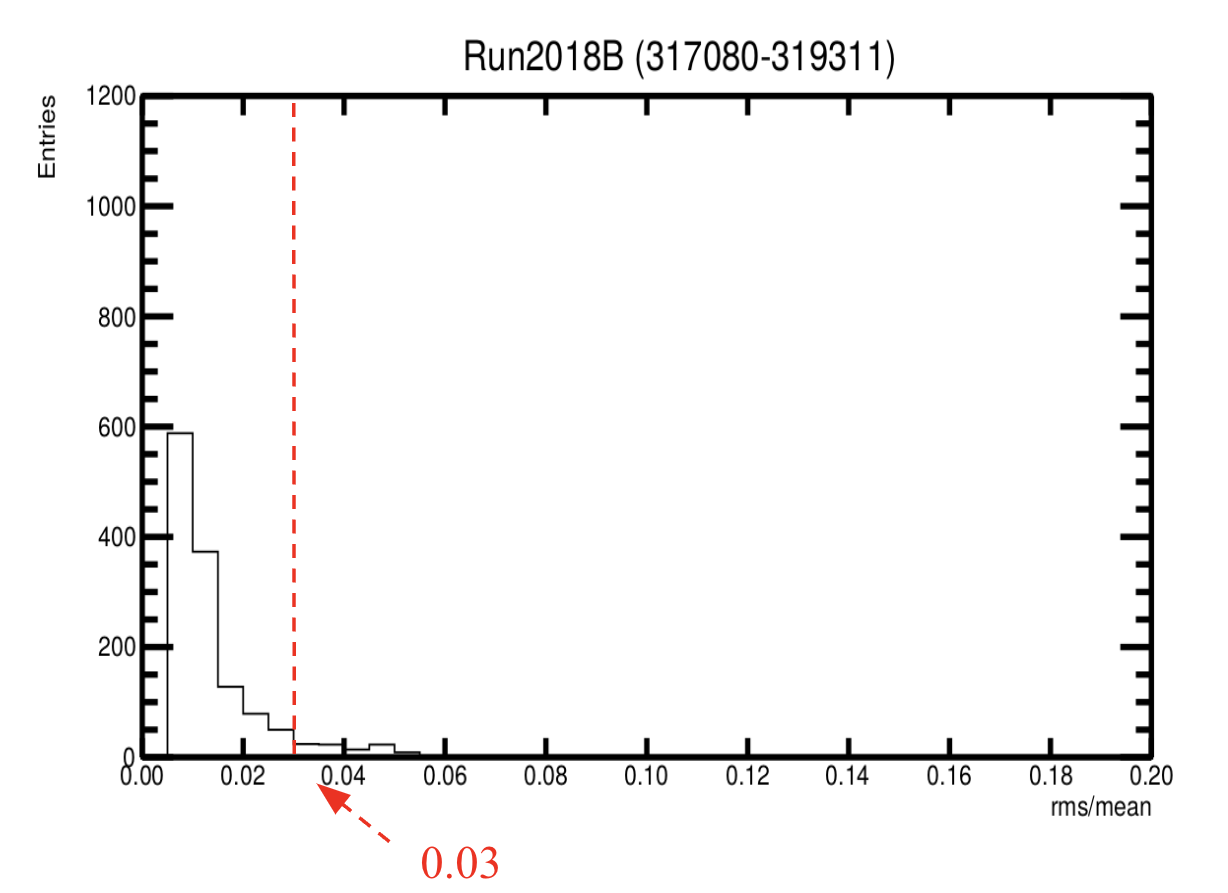
\includegraphics[width=0.6\textwidth]{ashish_thesis/3percent_cut.png}
\caption[Second Iteration For Outlier Module Removal]{%                                                                                                                                                                                       
 Second selection on RMS/mean of 3\% is applied to obtain module veto list for each period.
}
\label{fig:second_it_cut}
\end{figure}


\begin{figure}[!htp]
\centering
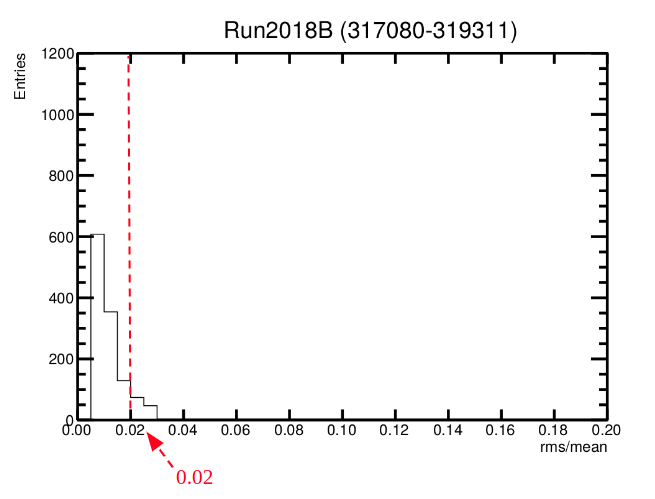
\includegraphics[width=0.6\textwidth]{ashish_thesis/second_iteration_cut.png}
\caption[Final Iteration For Outlier Module Removal]{%
 Final selection on RMS/mean of 2\% is applied to obtain module veto list for each period.
}
\label{fig:sec_it_cut}
\end{figure}

\end{comment}

%\begin{figure}[!htp]
%\centering
%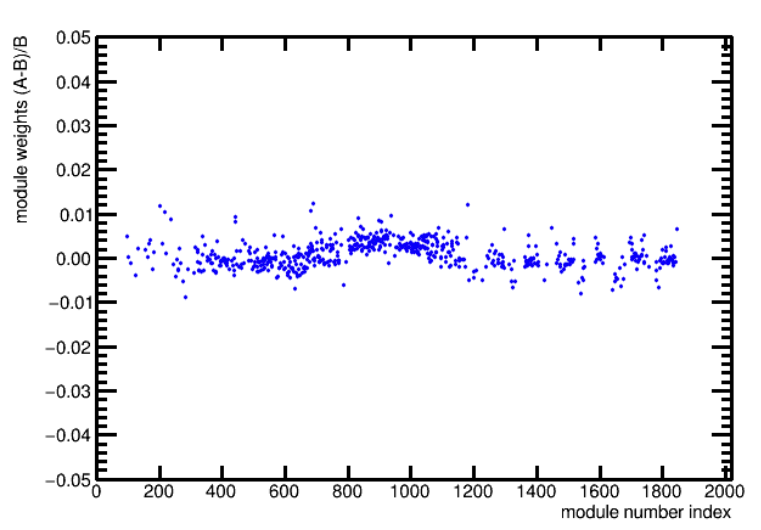
\includegraphics[width=1\textwidth]{ashish_thesis/mod_weight_comparison.png}
%\caption{%
%   Change in module weights between period A and B for all modules left after applying 2\% rms module vetolist.
%}
%\label{fig:mod_w_com}
%\end{figure}


\begin{figure}[!htp]
\centering
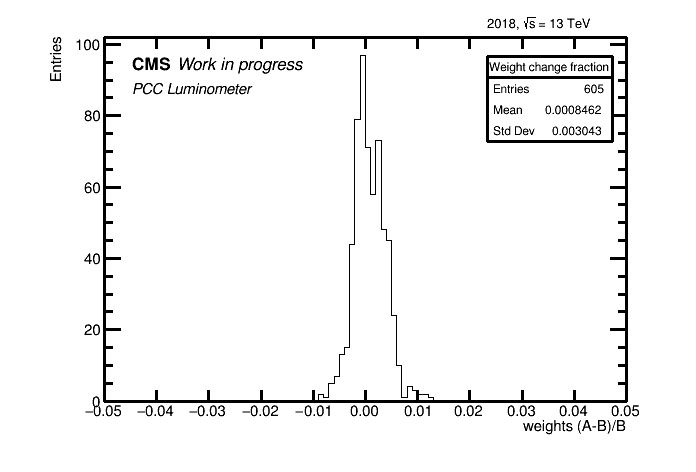
\includegraphics[width=0.7\textwidth]{ashish_thesis/mod_weight_comp_2.png}
\caption[Module Weights Change Removal]{%
   Projection of change in module weights between period A and B. Modules showing more than 3 sigma change in module weights are added to the module veto list.
}
\label{fig:mod_w_com_1}
\end{figure}
   
 2\% selection on RMS/mean of module weights gives the best stability for all pixel detector barrel layers and forward disks. Number of good and bad modules after this selection is shown in Table \ref{tab:per period veto}. % Bad modules found after applying this 2\% selection in the final iterative step are used to constitute a 2 $\%$ rms module veto list for each period as shown in Table \ref{tab:per period veto}. 
                                                                                 
 \begin{table}
   \begin{center}
     \caption[Good/bad modules for each period]{2 \% rms module veto list for each period showing number of good and bad modules.}
    \begin{tabular}{ccccc}  
    \textbf{Period}   & \textbf{\# bad modules} & \textbf{\# good modules} \\ \hline
     A      &   1276   &  580    \\  
     B      &    802  &     1054  \\ 
     C      &   1076  &    780   \\ 
     D1     &  1169  &     687  \\ 
     D2     &  1184  &    672   \\ 
     D3     &  1081  &    775   \\ 
     D4     &  1032  &     824  \\ 
      \end{tabular}
    %\caption[Good and bad modules during each period]{2 \% rms module veto list for each period showing number of good and bad modules.}
    \label{tab:per period veto}
  \end{center}
\end{table}


\begin{comment}

Table \ref{tab:pccvis_diffveto} depicts the mean and RMS values of PCC/HFOC luminosity for each period using per period veto list. The mean values are demonstrated for periods A, B, C, D1, D2, D3, and D4, with 'A' having a mean value of 1.006 and the other periods ranging from 0.9981 to 1.003. The RMS values range from 0.002115 to 0.004183, showing a degree of variation. The table also provides the ratio of RMS to mean, which offers a perspective on relative fluctuations. The calculated ratios are close to their corresponding RMS values, indicating relatively consistent variability across periods. The table effectively illustrates a nuanced variation in mean luminosity values across different periods.

\begin{table}[!ht]
\centering
%\topcaption{%
 %PCC/ HFOC luminosity mean and rms values for new per period vetolist showing variation in mean values across period.
%}
\begin{tabular}{ccccc}
    \textbf{Period} & \textbf{mean} & \textbf{rms} &  \textbf{rms/mean} \\ \hline
    A & 1.006 & 0.004183 & 0.004158 \\
    B & 0.9981  & 0.003133 & 0.0031389 \\
    C & 0.9989  & 0.003009 & 0.003012\\
    D1 & 1.003  & 0.002441 & 0.002433 \\
    D2 & 1.001  & 0.0029 & 0.00289 \\
   D3  & 1  & 0.002115 & 0.002115 \\
   D4  & 1.002  & 0.003673 & 0.003666 \\ 
\end{tabular}
\caption[Mean value change for PCC/HFOC across period.]{%                                                                                                                                       
 PCC/ HFOC luminosity mean and rms values for  per period veto list showing variation in mean values across period.
}
\label{tab:pccvis_diffveto}
\end{table}


\end{comment}

Figure \ref{fig:b_a_stability_vdm} shows the stability plots of the relative contribution to luminosity from pixel layers/disks before and after applying the module veto in the vdM calibration period. %This veto list application is essential for maintaining data quality as it helps to filter out data from modules showing more than 2\% variability in their RMS/mean, considered potentially large.
The plots provide a comparative view of how the luminosity fraction has been impacted by the application of this veto list. The 'before' plot shows greater variability, reflecting the fluctuations in luminosity across different layers or disks  during each lumi section. In contrast, the 'after' plot  display a more stable profile, indicating that the module selection has effectively reduced the variance in luminosity fraction readings, enhancing data stability. %This figure plays a crucial role in visualizing the impact of implementing stringent data vetting procedures in the analysis of luminosity measurement.
%An improvement in the stability of various PCC layer and disk for the whole Period B after applying new veto list shown in Fig. \ref{fig:old_new_periodB}.

\begin{figure}[!htp]
\centering
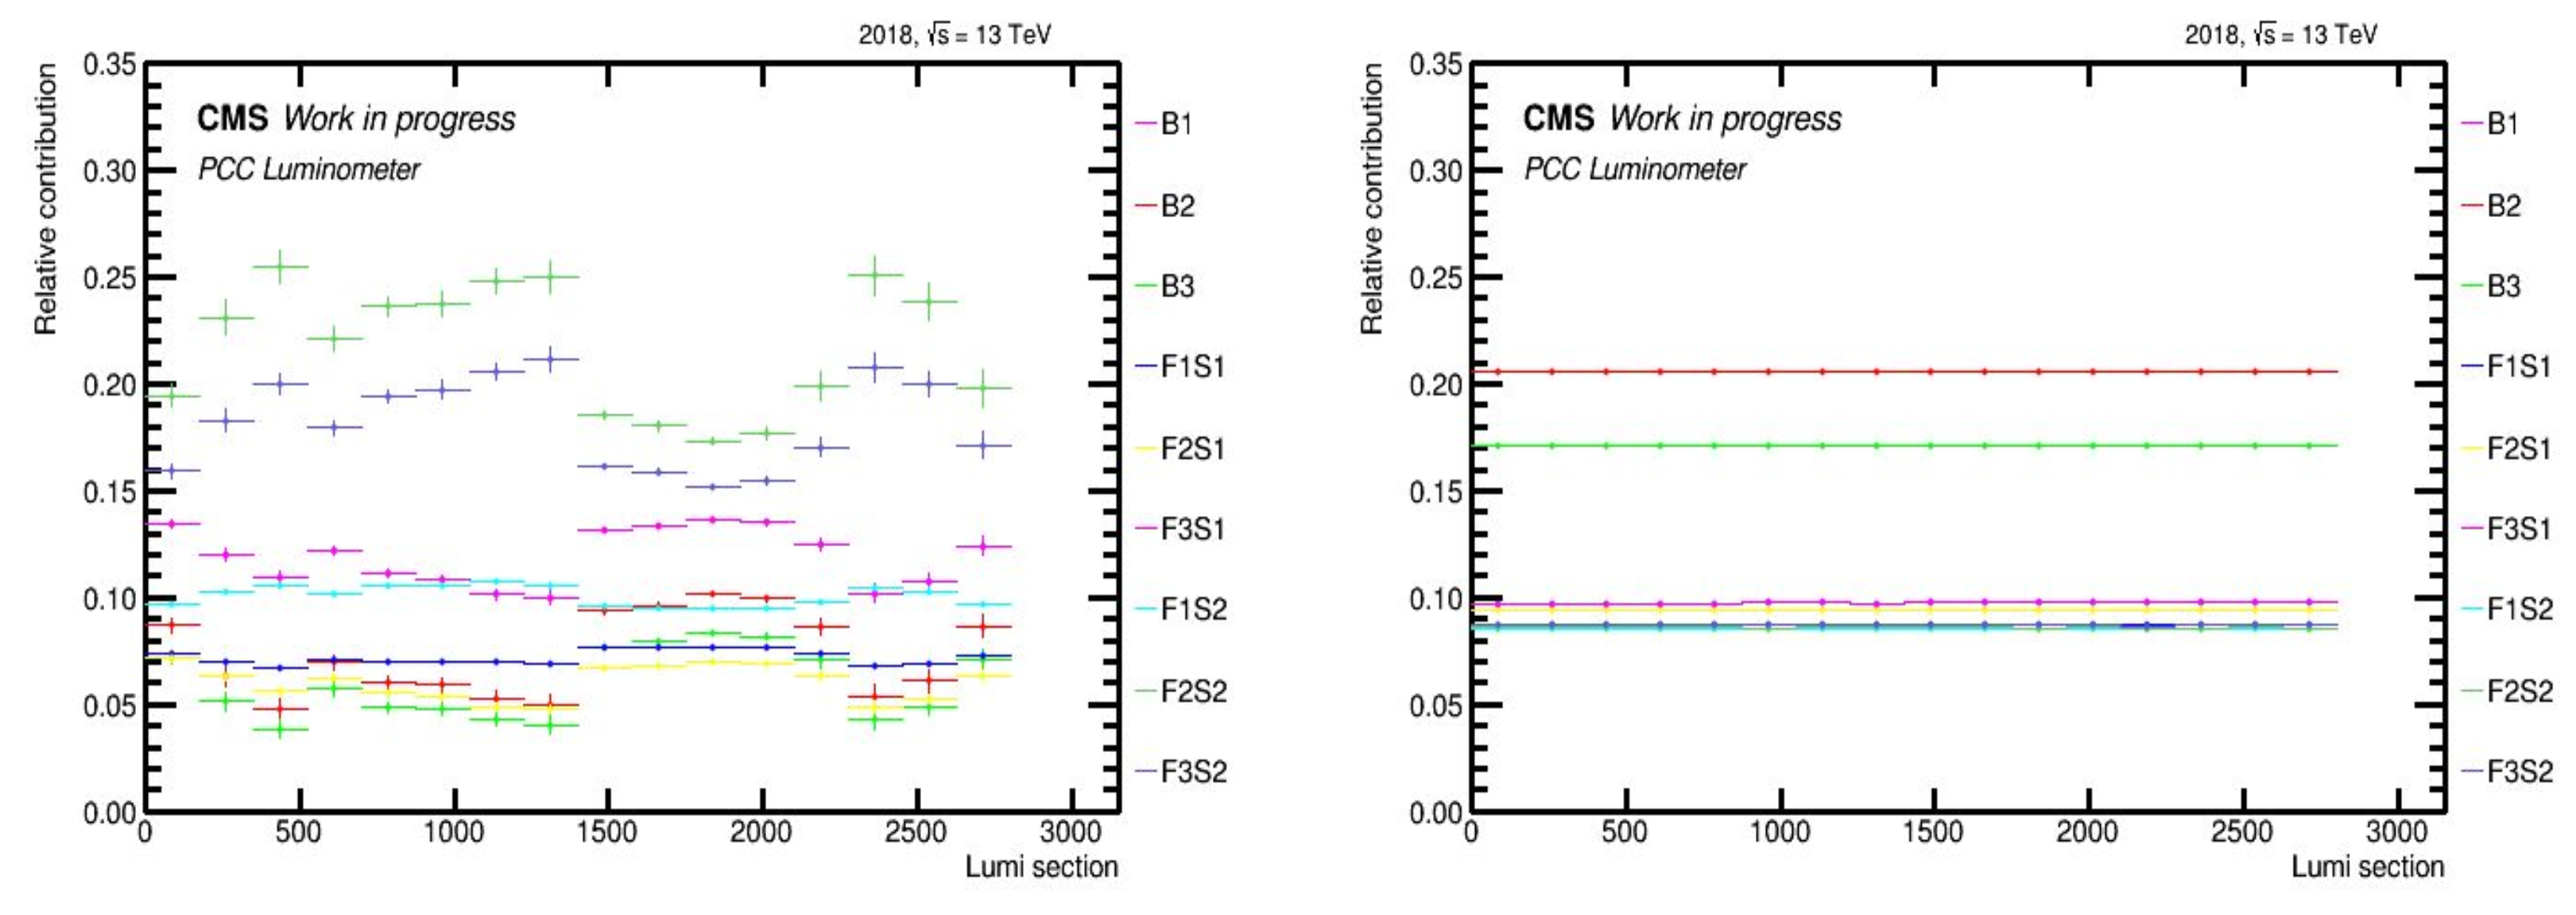
\includegraphics[width=1\textwidth]{ashish_thesis/before_after_vdm_stability_1.png}
\caption[PCC vdM Stability]{%                                                                                                                                                                      
   Luminosity fraction per layer or disk (stability plots) before (no veto) and after applying the final module veto with 2\% RMS/mean selection for the vdM fill data.
}
\label{fig:b_a_stability_vdm}
\end{figure}

%\begin{figure}[!htp]
%\centering
%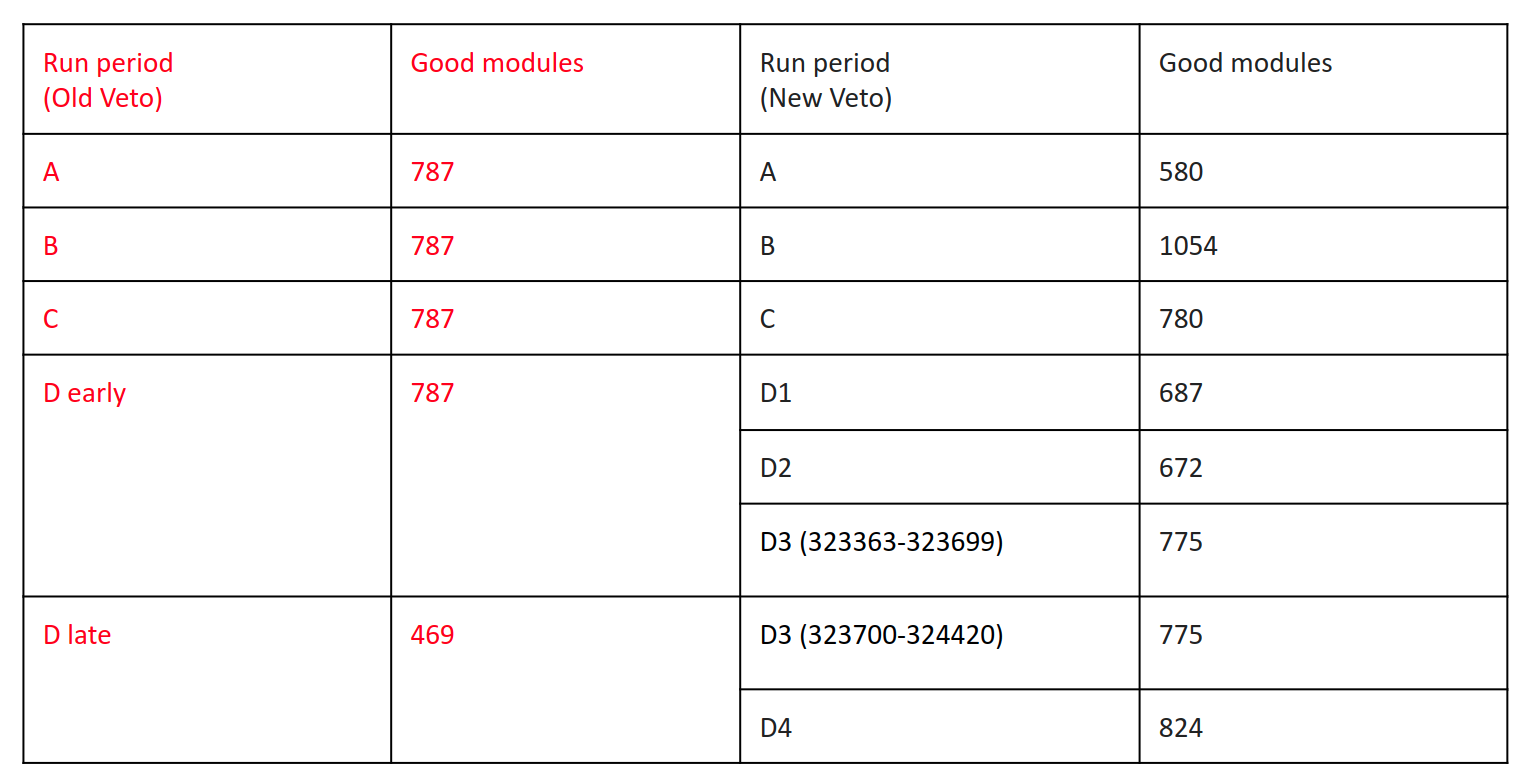
\includegraphics[width=0.8\textwidth]{ashish_thesis/old_new_veto.png}
%\caption{%
 %  klm
%}
%\label{fig:old_new_vetolist}
%\end{figure}

\begin{comment}
  
Table \ref{tab:runperiod_oldnew} details the number of "Good Modules" across different run periods under both old and new veto conditions. The periods under consideration are A, B, C, and D, with D further subdivided into "early" and "late" phases for the old veto. In the new veto, period D is segmented into D1, D2, D3 (split into two specific run ranges), and D4. Under the "Old Veto" condition, periods A, B, C, and "D early" each have a consistent count of 787 good modules. However, for the "D late" phase, there are 469 good modules, suggesting a notable reduction from the earlier phase of period D. Moving to the "New Veto" scenario, the good modules count shows considerable variability across periods. Period A records 580 good modules, B has the highest number with 1054, and C presents 780 good modules. For the D period under the new veto, D1 and D2 show 687 and 672 good modules respectively. Period D3, divided into two separate run ranges (323363-323699 and 323700-324420), maintains a consistent count of 775 good modules for both ranges. Finally, for period D4, there are 824 good modules.

\begin{table}
  \centering
  \caption{Run Period and Good Modules}
\begin{tabular}{cccc}
\textbf{Run period (Old Veto)} & \textbf{Good modules} & \textbf{Run period (New Veto)} & \textbf{Good modules} \\
\hline
A & 787 & A & 580 \\
B & 787 & B & 1054 \\
C & 787 & C & 780 \\
D early & 787 & D1 & 687 \\
 & & D2 & 672 \\
 &  & D3 (323363-323699)  &  775\\
D late & 469 & D3 (323700-324420) & 775 \\
&  & D4 & 824\\
\end{tabular}
%\caption{Run Period and Good Modules}
\label{tab:runperiod_oldnew}
\end{table}

\end{comment}

%An improvement in the stability of various PCC layer and disk is shown in Fig. \ref{fig:old_new_periodB} after applying new veto list.

%\begin{figure}[!htp]
%\centering
%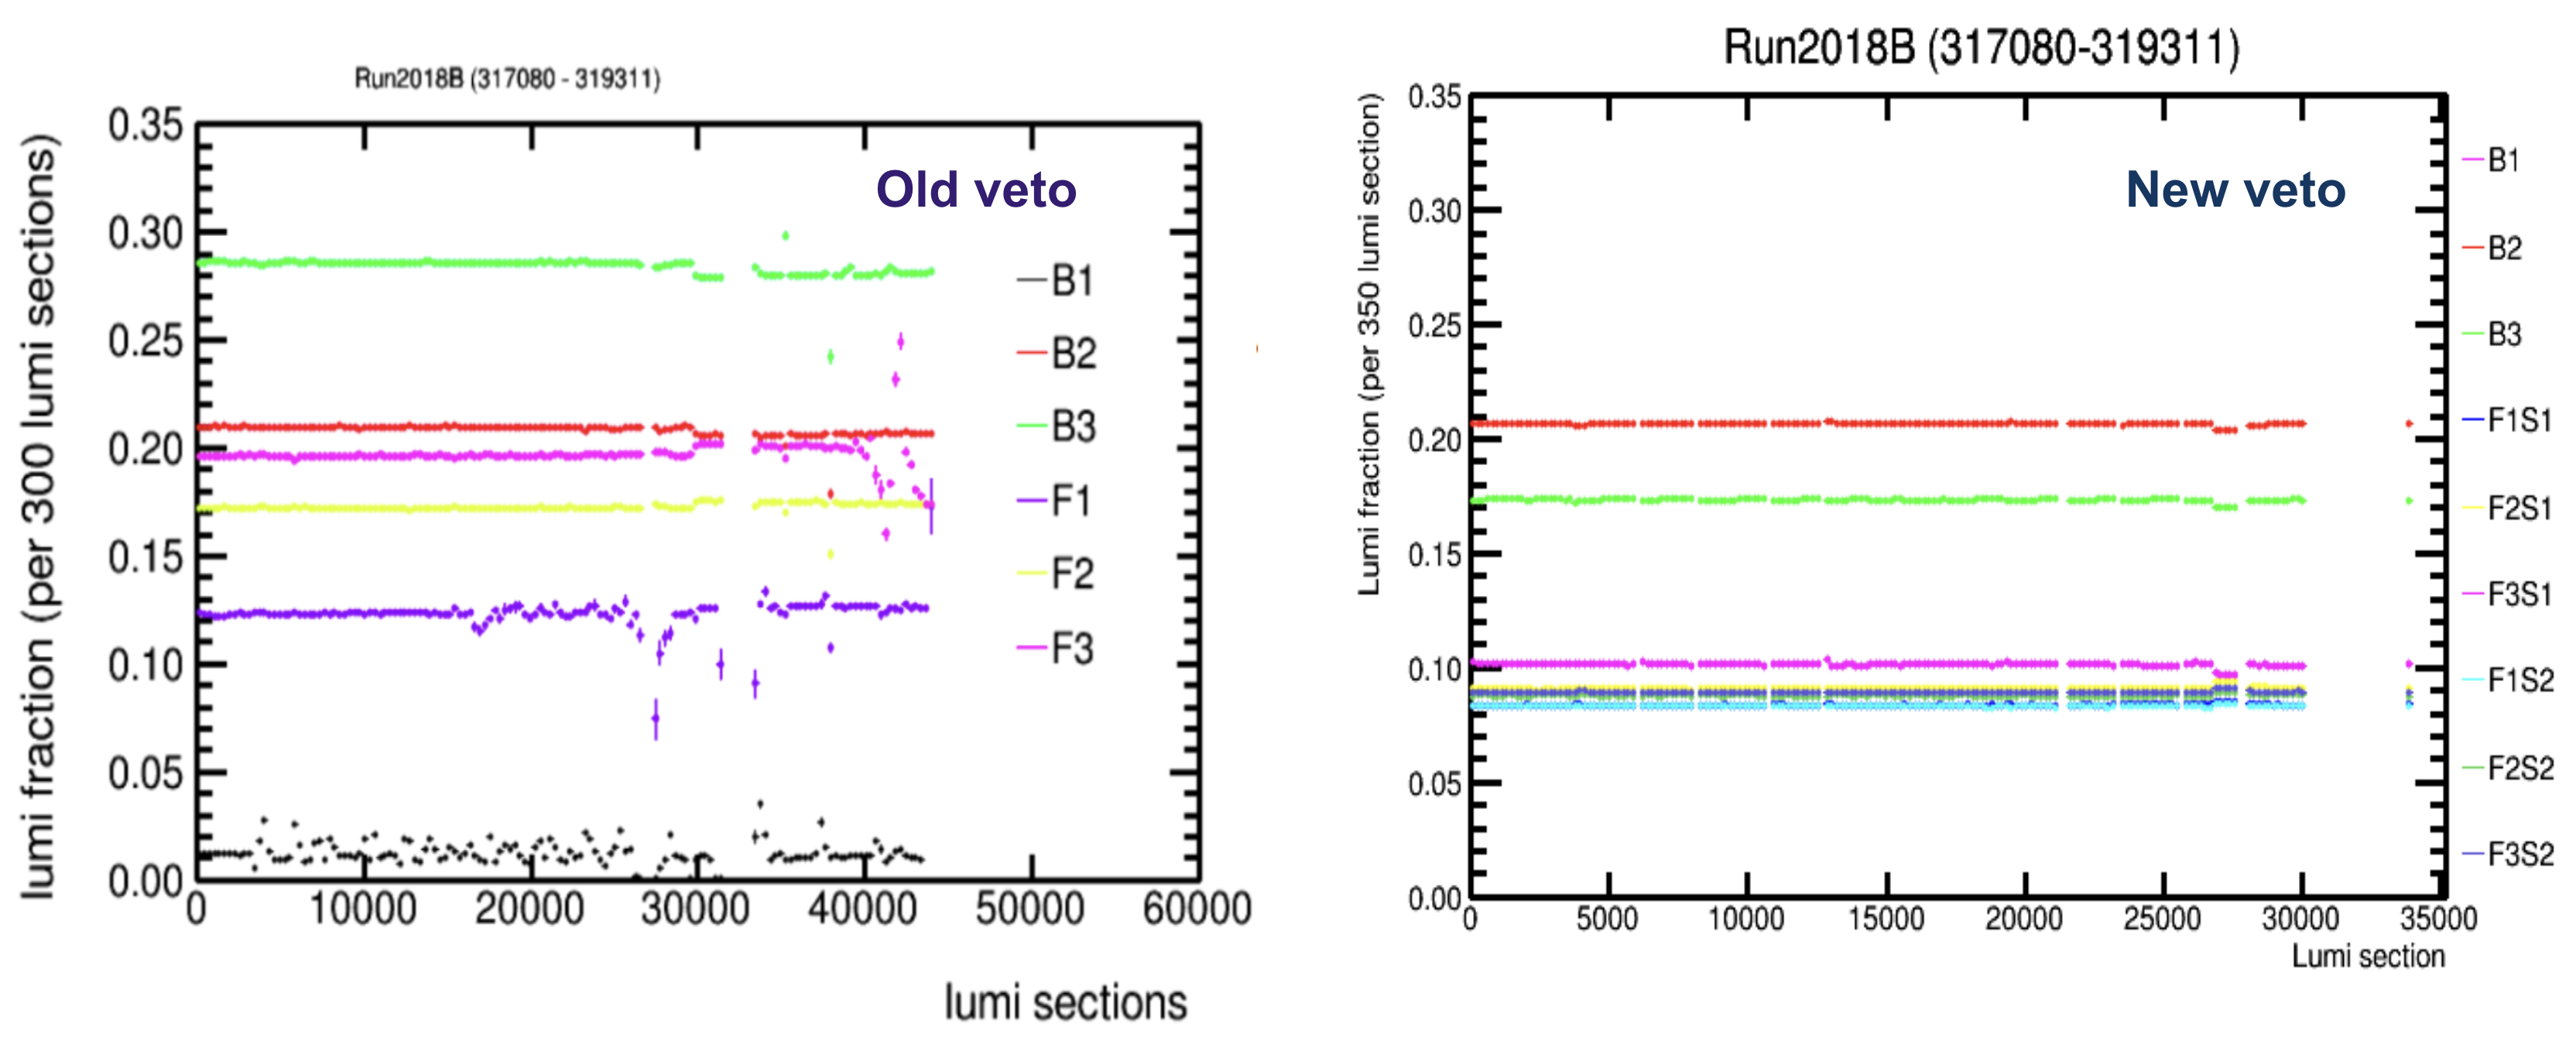
\includegraphics[width=1\textwidth]{ashish_thesis/old_new_veto_periodB.png}
%\caption[Old new veto period B per layer/disk stability]{Comparison of PCC layer and disk stability for old and new module veto.}
%\label{fig:old_new_periodB}
%\end{figure}

%To reduce the variation in mean values across periods thereby improving the stability of PCC luminometer, a common module veto list is created using the 2\% RMS/mean selection as shown in Table \ref{tab:2commonveto}.

Table \ref{tab:2commonveto} shows the number of modules for a common selection over the entire year. Common module veto list is a combination of module veto list of all run periods A, B, C, D1, D2, D3 and D4. Approach to make a common module veto list is to start by combining module vetolists of period A,B and C, then combine A,B, C, D1 and so on. Less than $9\%$ of the pixel modules remain after applying module stability selections to be used for final luminosity measurement. The total number of good modules across all layers and disks is 155.


\begin{table}
  \begin{center}
    \caption[Common module veto list]{Final module veto list. This veto list is created by combining module veto lists for each period.}
    \begin{tabular}{ccccc}  
      \textbf{Period}   & \textbf{\# bad modules} & \textbf{\# good modules} \\  \hline
      A + B  & 1276 & 580 \\
     A + B + C      &  1417   &  439    \\  
     A + B + C + D1      &   1534  &   322    \\ 
     A + B + C + D1 + D2      &   1629 &    227   \\ 
     A + B + C + D1 + D2 + D3     &   1668 &   188    \\ 
     A + B + C + D1 + D2 + D3 + D4     &  1701 &     155  \\ 
      \end{tabular}
    %\caption[Common module veto list for all periods]{Final module veto list. This veto list is created by combining module veto lists for each period.}
    \label{tab:2commonveto}
  \end{center}
\end{table}

%\begin{figure}[!htp]
%\centering
%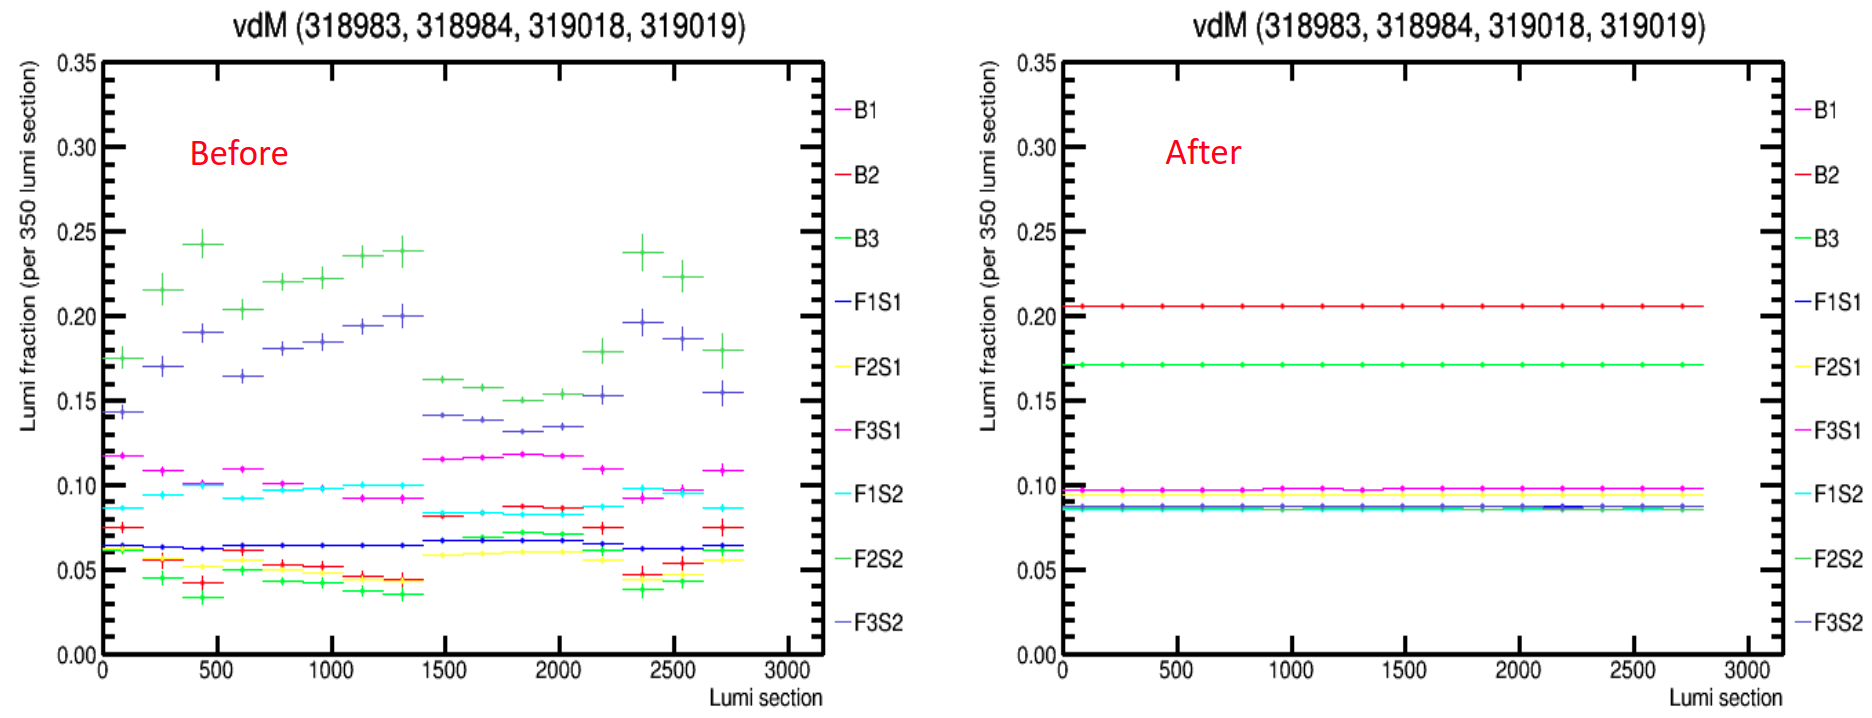
\includegraphics[width=1\textwidth]{ashish_thesis/before_after_vdm_stability.png}
%\caption[]{%
 %  Luminosity fraction (stability plots) before and after applying 2\% rms module vetolist.
%}
%\label{fig:b_a_stability_vdm}
%\end{figure}

%\begin{figure}[!htp]
%\centering
%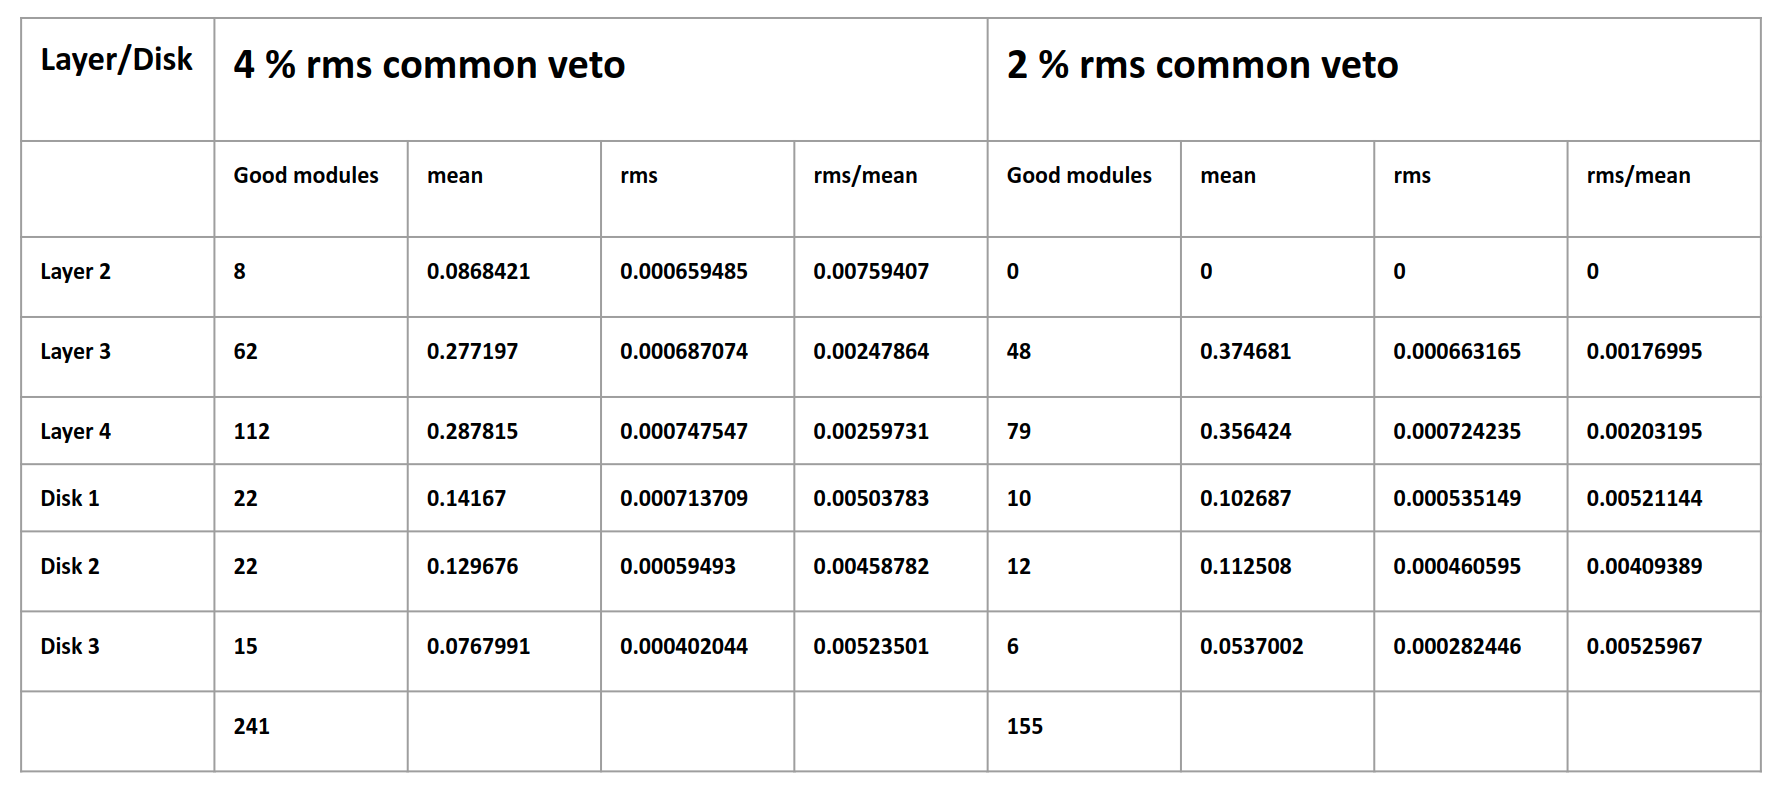
\includegraphics[width=1\textwidth]{ashish_thesis/pcc_layer_disk_mean_rms.png}
%\caption{%
%pcc layer disk mean rms
%}
%\label{fig:pixellalyerdiskmeanrms}
%\end{figure}

%\begin{table}[htbp]
%\centering
%\caption{Layer/Disk Statistics}
%\label{tab:layer-disk}
%\begin{tabular}{cccccc}
%\textbf{Layer/Disk} & \textbf{Good modules} & \textbf{mean} & \textbf{rms} & \textbf{rms/mean} \\
%\hline
%Layer 2 & 0 & 0 & 0 & 0 \\
%Layer 3 & 48 & 0.374681 & 0.000663165 & 0.00176995 \\
%Layer 4 & 79 & 0.356424 & 0.000724235 & 0.00203195 \\
%Disk 1 & 10 & 0.102687 & 0.000535149 & 0.00521144 \\
%Disk 2 & 12 & 0.112508 & 0.000460595 & 0.00409389 \\
%Disk 3 & 6 & 0.0537002 & 0.000282446 & 0.00525967 \\
%Total  & 155 & & \\
%\multicolumn{2}{c}{} & \multicolumn{2}{r}{155} \\
%\end{tabular}
%\caption{Layer/Disk Statistics}
%\end{table}

The relative contribution to PCC luminosity from each pixel detector layer and disk without and with final module veto list is shown in Fig. \ref{fig:stabprof_4333}.

%\begin{figure}[!htp]
%\centering
%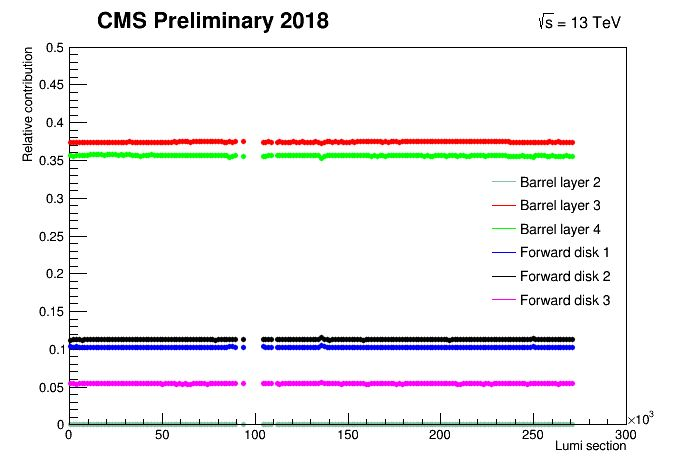
\includegraphics[width=0.8\textwidth]{ashish_thesis/2percentcommonveto_pixellayerdisk.png}
%\caption[Pixel layer/disk stability]{%
 %  Stability profiles of pixel detector layer and disk modules for 2\% rms common module veto list.
%}
%\label{fig:stabprof}
%\end{figure}

\begin{figure}[!htp]
\centering
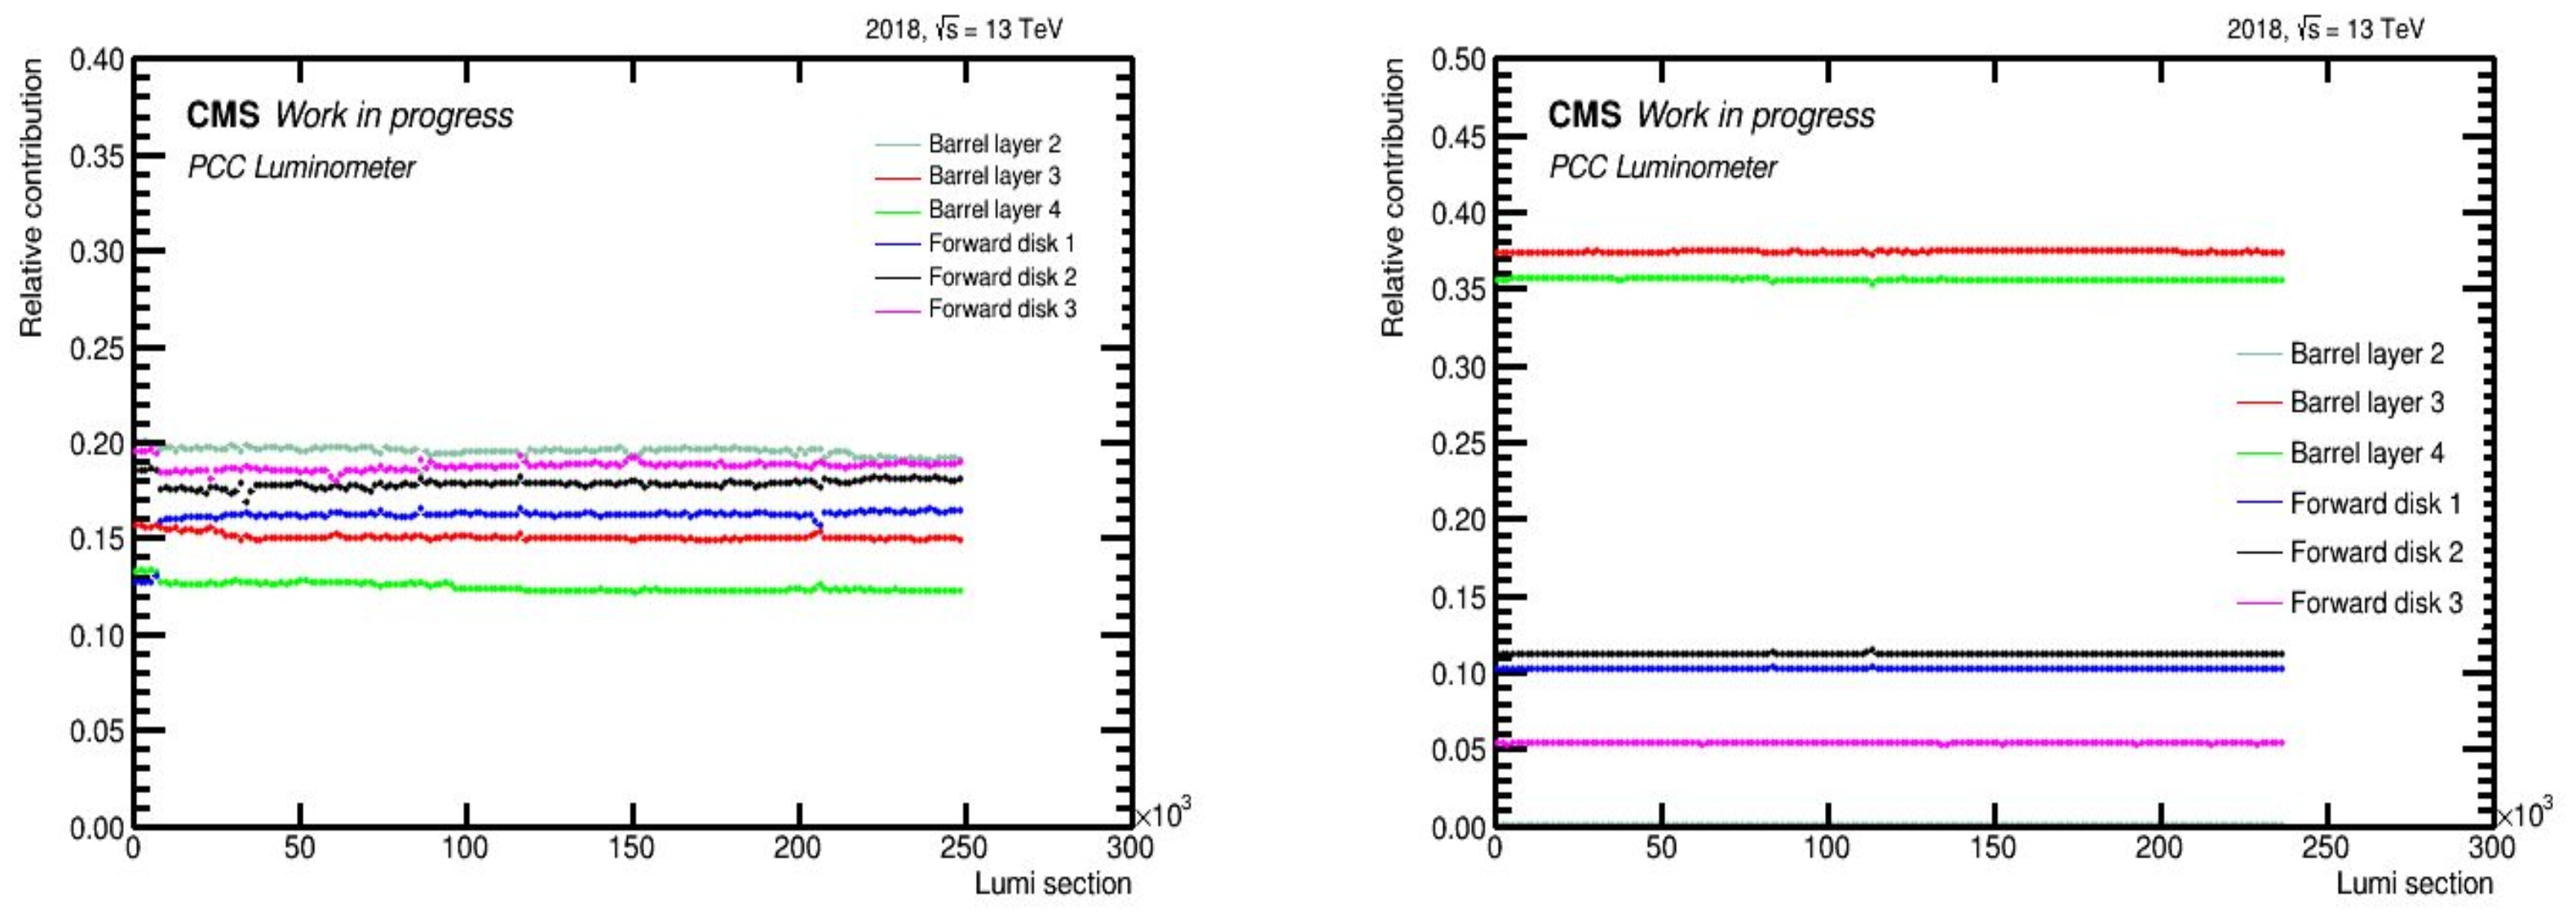
\includegraphics[width=\textwidth]{ashish_thesis/2percentcommonveto_pixellayerdisk_1.png}
\caption[PCC Stability For Physics Runs]{Left: Luminosity fraction of pixel detector for various layer and disks as a function of lumi section for a module selection excluding only the BPIX Layer 0 for the full 2018 zero-bias dataset. Right: Stability profiles of pixel detector layer and disk for final module veto list.}
\label{fig:stabprof_4333}
\end{figure}

%\begin{figure}[!htp]
 % \centering
  %\begin{subfigure}[b]{0.49\textwidth}
   % 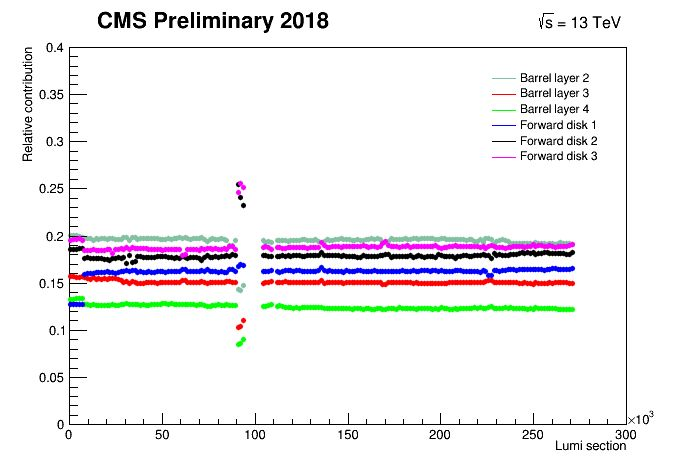
\includegraphics[width=\textwidth]{ashish_thesis/pixel_layer_disk_B0_veto.png}
    %\caption{Image 1}
  %\end{subfigure}
  %\hfill % or \hspace{5mm} for a specific horizontal space
  %\begin{subfigure}[b]{0.49\textwidth}
   % 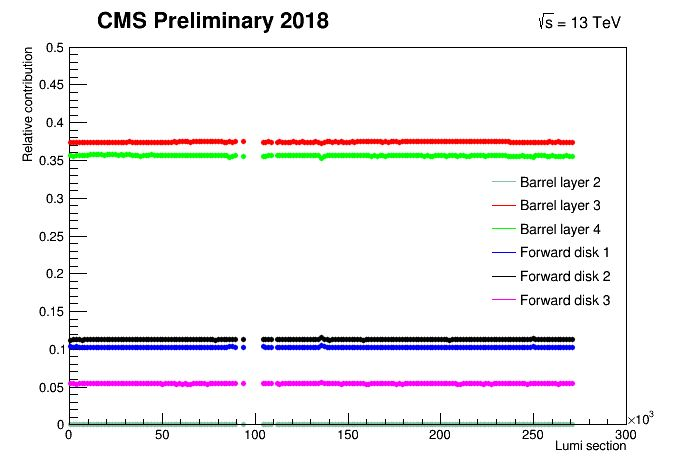
\includegraphics[width=\textwidth]{ashish_thesis/2percentcommonveto_pixellayerdisk.png}
    %\caption{Image 2}
  %\end{subfigure}
  %%\caption[PCC Stability For Physics Runs]{Left: Luminosity fraction of pixel detector for various layer and disks as a function of lumi section for a module selection excluding only the BPIX Layer 0 for the full 2018 zero-bias dataset. Right: Stability profiles of pixel detector layer and disk for final module veto list.}
  %\label{fig:stabprof_4333}
%\end{figure}

Table \ref{tab:layer-disk} presents the statistics of good modules across different layers and disks for final module veto list. The layers and disks are divided into five categories: Layer 3, Layer 4, Disk 1, Disk 2, and Disk 3. For each of these categories, the number of good modules, mean, RMS, and the ratio of RMS to mean are provided. Layer 2 has no good modules. %and all statistical parameters are zero.
Layer 3, on the other hand, has 48 good modules with a mean value of 0.374681, an RMS of 0.000663165 and an RMS-to-mean ratio of 0.00176995, indicating low variability. Layer 4 shows a slightly larger count of good modules with 79, and similar statistical parameters to Layer 3, albeit with a slightly higher RMS and RMS-to-mean ratio, suggesting slightly greater variability. When it comes to the disk categories, Disk 1 and Disk 2 each have 10 and 12 good modules respectively. Their mean values are lower than those of the layers, as are their RMS values, although their RMS-to-mean ratios are higher, suggesting greater relative variability in these categories. Disk 3 has the fewest good modules with only 6, and it presents the highest RMS-to-mean ratio among all categories, indicating the highest relative variability. %The total number of good modules across all layers and disks is 155.
%It's noteworthy that the table does not provide an aggregated mean, RMS, or RMS-to-mean ratio across all categories.

\begin{table}[!htp]
  \centering
  \caption[Final module veto statistics]{Layer/Disk good modules and statistics for final module veto list.}
%\caption{Layer/Disk Statistics}                                                                                                                                                                       
%\label{tab:layer-disk}
\begin{tabular}{cccccc}
\textbf{Layer/Disk} & \textbf{Good modules} & \textbf{mean} & \textbf{rms} & \textbf{rms/mean} (\%) \\
\hline
Layer 3 & 48 & 0.374681 & 0.000663165 & 0.176995 \\
Layer 4 & 79 & 0.356424 & 0.000724235 & 0.203195 \\
Disk 1 & 10 & 0.102687 & 0.000535149 & 0.521144 \\
Disk 2 & 12 & 0.112508 & 0.000460595 & 0.409389 \\
Disk 3 & 6 & 0.0537002 & 0.000282446 & 0.525967 \\
Total  & 155 & & \\
%\multicolumn{2}{c}{} & \multicolumn{2}{r}{155} \\                                                                                                                            
\end{tabular}
%\caption[Final veto statistics]{Layer/Disk good modules and statistics for final module veto list.}
\label{tab:layer-disk}
\end{table}

\section{vdM calibration results}

The calibration of luminosity measurement by the CMS experiment luminometers in the 2018 proton-proton data taking at $\sqrt{s}$ = 13 TeV \cite{pas_18} was performed during LHC fill 6868 on June 30 and July 1, 2018 at $\sqrt{s}$ = 13 TeV. Zero-bias triggers on 5 bunch pairs (BCIDs 265, 865, 1780, 2192, and 3380) recorded events rate is 27.7 kHz. Trigger is applied on five colliding bunches due to limitation of the recording bandwidth.

%\item "lsc1", was the "constant separation" scan, two beams were separated by 1.4 $\sigma$ and moved together in steps of 1 $\sigma$ across and back. %\item "lsc2", was the "variable separation" scan method, one beam (starting with beam 1) is moved to -2.5 $\sigma$ and then a three-point scan (a "miniscan") is performed with the other beam.                         %a normal VdM scan pair "norm4" and two short emittance scan pairs "emit4" and "emit5" were also performed.     %The 2018 CMS VdM scan program was conducted in two segments, interrupted by an alarm. The first segment involved six x-y scan pairs. Two were short ``emittance'' scans, named ``emit1'' and ``emit2,'' where the beamswere separated by $ \(4\sigma_b\) $ over 9 steps with a 10 second integration time at each step. A standard VdM scan, named ``norm1,'' separated the beams by $\(6\sigma_b \approx 600\)~\mu m$ in 25 steps, with a 30-second duration per step. The ``offset1'' scan followed the same procedure as the standard scans but with a $\(\pm 1.5\sigma_b\)$ separation in the non-scanning direction. Lastly, two sets of ``beam imaging'' scans wereconducted, where one beam remained fixed while the other was moved in 19 steps between $\(+4.5\sigma_b\)$ and $\(-4.5\sigma_b\)$, each lasting 46 seconds per step.                                                      
The 2018 CMS vdM scan program (shown in Fig. \ref{fig:vdm_prog_2018}) was conducted in two segments, interrupted by an alarm. The first segment involved six x-y scan pairs. Two were short ``emittance'' scans, named ``emit1'' and ``emit2,'' where the beams were separated by \(4\sigma_b\) over 9 steps with a 10-second integration time at each step. A standard vdM scan (described in section 3.1), named ``vdM1,'' separated the beams by \(6\sigma_b \approx 600\)~$\mu$m in 25 steps, with a 30-second duration per step. The ``offset1'' scan followed the same procedure as the standard scans but with a \(\pm 1.5\sigma_b\) separation in the non-scanningdirection. Lastly, two sets of ``beam imaging'' scans were conducted, where one beam remained fixed while the other was moved in 19 steps between \(+4.5\sigma_b\) and \(-4.5\sigma_b\), each lasting 46 seconds per step. The second part of the scan program was conducted in the same fill, approximately 7.5 hours later, and consisted of twelve scan pairs. This included a short emittance scan, ``emit3''; beam imaging scan pairs, ``imag2'' and``imag3''; an offset scan pair, ``offset2''; and two standard vdM scan pairs, ``vdM2'' and ``vdM3''.

Beam Imaging Scans: Beam imaging scans are designed to measure the transverse profile of the beam. They involve moving one beam across the other in steps and measuring the interaction rate (or event rate) at each step. By doing this, the shape or "profile" of the beam in the transverse plane can be obtained. These scans allow for a detailed analysis of the beam shape, which is essential for understanding the beam properties. In a perfect scenario, the density distributions of protons in a bunch would factorize into separate X (horizontal) and Y (vertical) components. However, real beams can have correlations between X and Y (non-factorization). Beam imaging scans help map the 2D profile of the beam and are thus essential for diagnosing and understanding any such correlations. Knowing the 2D profile of the beams is crucial when calculating luminosity, as assumptions made about the factorization of the beam profiles feed into these calculations. By using beam imaging scans, experimenters can assess the validity of the factorization assumption or correct for any observed non-factorization.

Offset Scans: %Offset scans are performed to check for systematic errors in the luminosity measurement, which may arise from various sources.
They are similar to standard VdM scans but involve an intentional offset in the non-scanning direction. By comparing the results of offset scans with the results of regular scans, one can identify and correct for any systematic discrepancies that are present. Offset scans can help to assess the sensitivity of the luminosity measurement to non-factorization in the transverse plane. For example, if there are correlations between the X and Y distributions of protons (i.e., non-factorization), this could in principle affect the shape of the beam overlap region in the collision point. Offset scans, by changing the relative position of the beams, can help to assess whether such non-factorization has a significant effect on the measured luminosity.

vdM scans are typically conducted at least once a year to ensure the luminometer is correctly calibrated. Results of these scans that is the visible cross section is used to normalize the data collected by the experiments during physics run.

\begin{figure}[!htp]
    \centering
    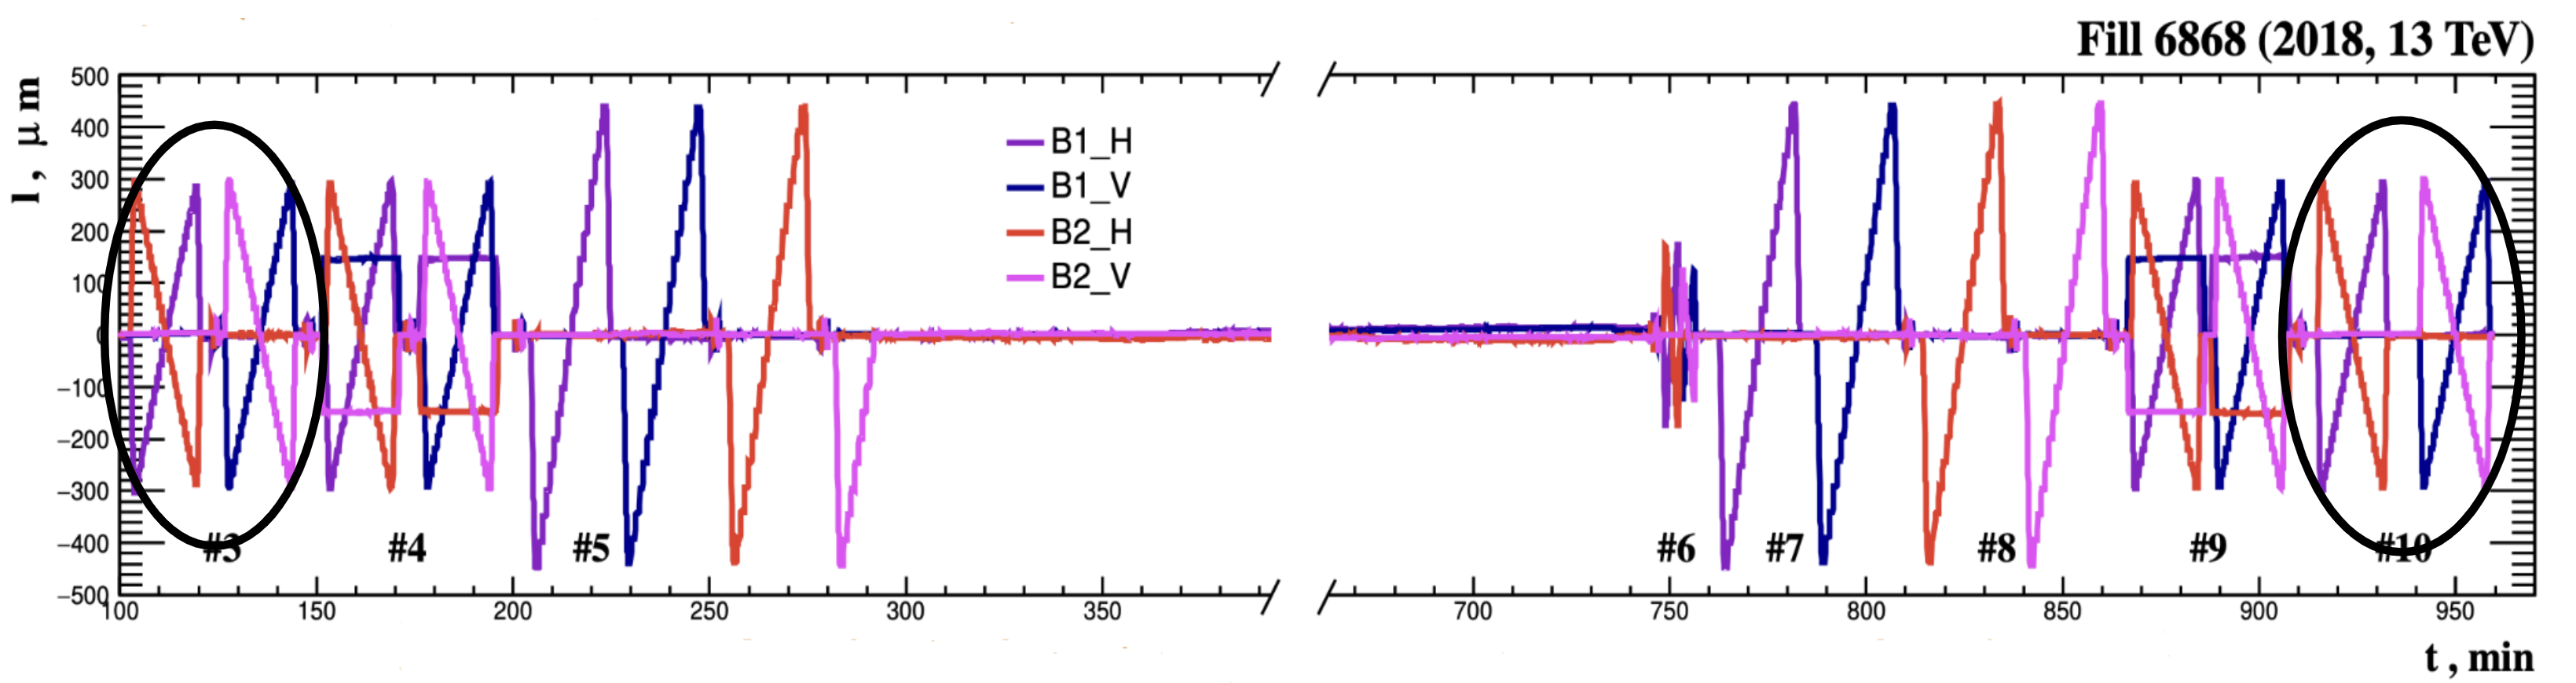
\includegraphics[width=1\textwidth]{ashish_thesis/vdm_program_2018.png}
    \caption[2018 vdM Program]{Beam position along x and y is plotted as a function of time showing different types of scans. #3 and #10 are vdM scans, #4 and #9 are offset scans, #5, #7 and #8 are beam imaging scans, #6 is emittance scan.}
    \label{fig:vdm_prog_2018}
\end{figure}

The vdM data (LHC fill 6868) is processed using the final module selection. The background estimation for the PCC rate is done with two super-separation scans SS1 and SS2. The mean and error are obtained from the $y$ projection of PCC per NB4 plotted as a function of time as shown in Fig. \ref{fig:sigmavis_ss_backg}. The results for five different BCIDs are shown in Table \ref{tab:vdm:SS1_SS2}, using the reprocessed PCC data for Fill 6868. The overall background correction applied to raw PCC rate is $0.02757\pm0.01987$, which is calculated by taking the average of the mean values of SS1 and SS2.


\begin{figure}[!htp]
\centering
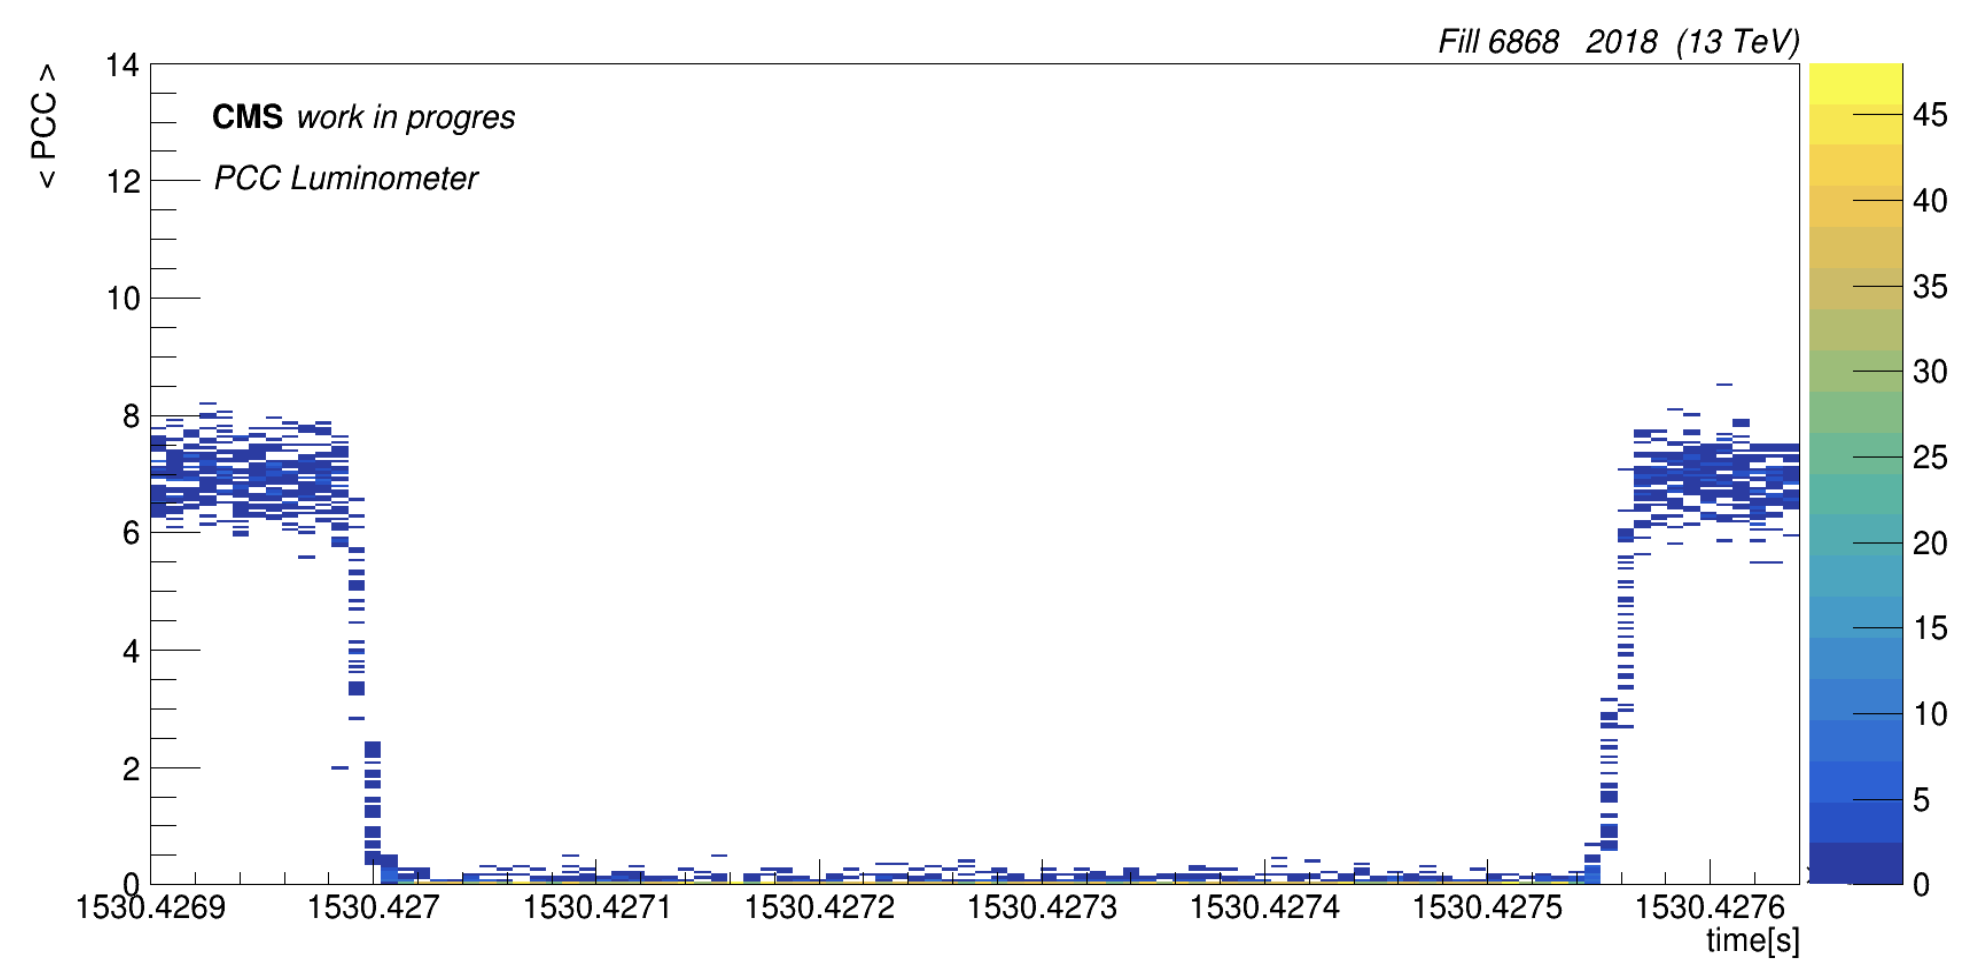
\includegraphics[width=1\textwidth]{ashish_thesis/SS1_SS2_bkg_pcc_1.png}
\caption[Background estimation]{2D histogram filled with the Avg. PCC evaluated per NB4, during head-on collisions (high part) and during the Super-Separation window (low part).}
\label{fig:sigmavis_ss_backg}
\end{figure}


\begin{table}
  \begin{center}
    \caption[2018 PCC Background]{Mean for the background estimated with the SS1 and SS2 data, separately for all five BCIDs and averaged.}
    \begin{tabular}{ccccc}
    \textbf{BCID}   & \textbf{Mean (SS1)} & \textbf{Mean (SS2)} \\ \hline
      265     &  0.02902    &  0.02743    \\
        865  &    0.02572  &     0.0281  \\
       1780    &  0.02862   &     0.0286  \\
       2192   &  0.02729  &     0.02323  \\
        3380  &  0.02882  &    0.02896   \\
      \end{tabular}
    %\caption[Background in PCC rate]{Mean for the background estimated with the SS1 and SS2 data, separately for all five BCIDs and averaged.}
    \label{tab:vdm:SS1_SS2}
  \end{center}
\end{table}

Figure \ref{fig:fitquality} displays the collision rates for a specific particle bunch as one beam is moved across another, with all necessary corrections applied. $\chi^2/ndof$ for vdM and imaging scans has an average value of 0.4514 where the Poly2G fit model converges for all BCIDs. Peak value and beam overlap $\Sigma_x$ and $\Sigma_y$ along X and Y are extracted from fit to calculate $\sigma_{vis}$. %The $\sigma_{vis}$ per scan is averaged over all BCIDs and its scan to scan variation is shown in Fig. \ref{fig:sigmaperscan}.
The $\sigma_{vis}$ value obtained by averaging all scans is for final module veto list is 960.54 $\pm$ 0.85(stat.) mb.

\begin{figure}[!htp]
    \centering
    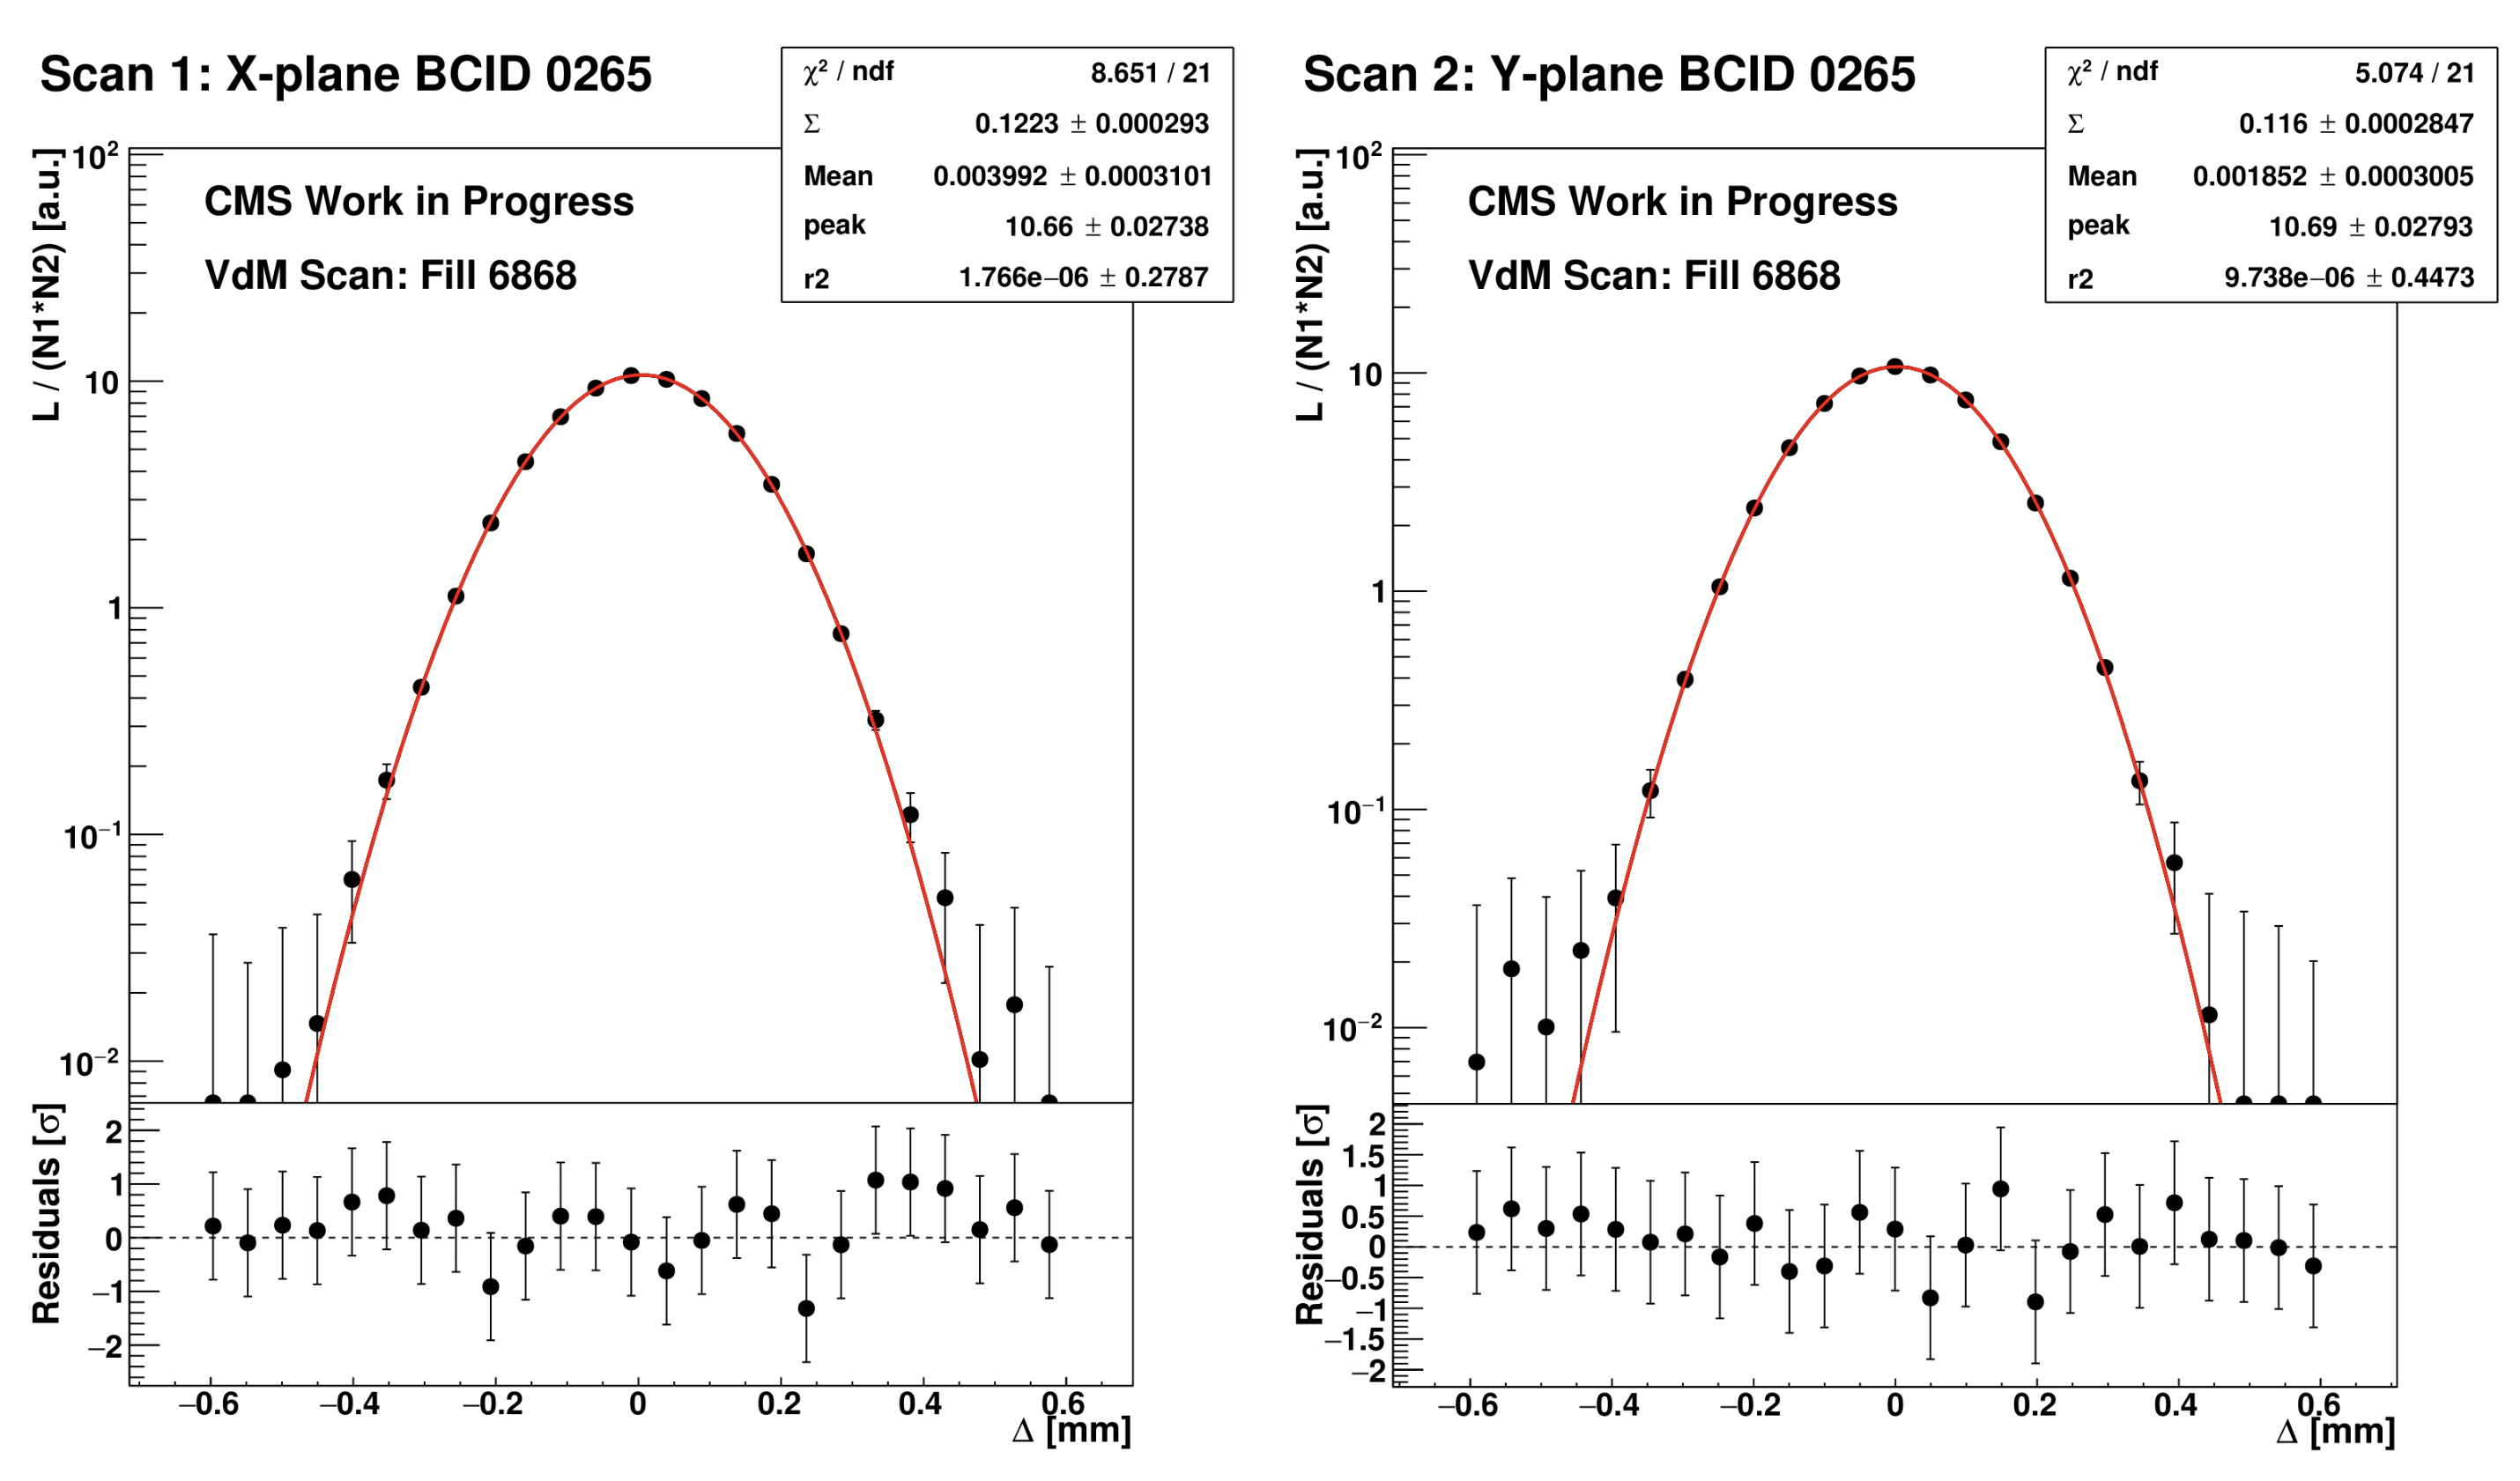
\includegraphics[width=1\textwidth]{ashish_thesis/vdM_fit_cveto_1.png}
    \caption[PCC Rate Fit]{Rates and the resulting fitted Poly2G scan curves as a function of the beam separation for a single bunch (BCID 265) as recorded by PCC for vdM1 scan in the x (left) and y direction (right). Background subtraction and the beam corrections have been applied to the raw data before the fit.}
    \label{fig:fitquality}
\end{figure}

%\begin{figure}[!htp]
 %   \centering
  %  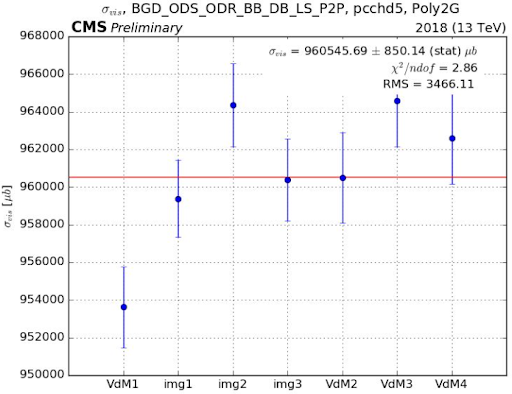
\includegraphics[width=0.8\textwidth]{ashish_thesis/sigma_vis_per_scan.png}
  %  \caption[PCC Visible Cross Section]{Visible cross section per scan where red line shows the average value.}
   % \label{fig:sigmaperscan}
%\end{figure}

PCC visible cross section for various bunch crossing across different scans is shown in Fig. \ref{fig:sigmavis_btob_variation}. The data points exhibit a scatter around the mean value, with no apparent systematic bias, as they are distributed both above and below this average. While there is a certain level of precision suggested by the proximity of the points to the mean line, the varying lengths of the error bars indicate a range in measurement uncertainty. This variability in precision could be attributed to fluctuating experimental conditions inherent to each BCID. %Overall, the experiment seems to have achieved a degree of accuracy, given that the measurements are clustered around the mean, yet the spread indicated by the error bars suggests that there is potential for optimizing the precision

\begin{figure}[!htp]
\centering
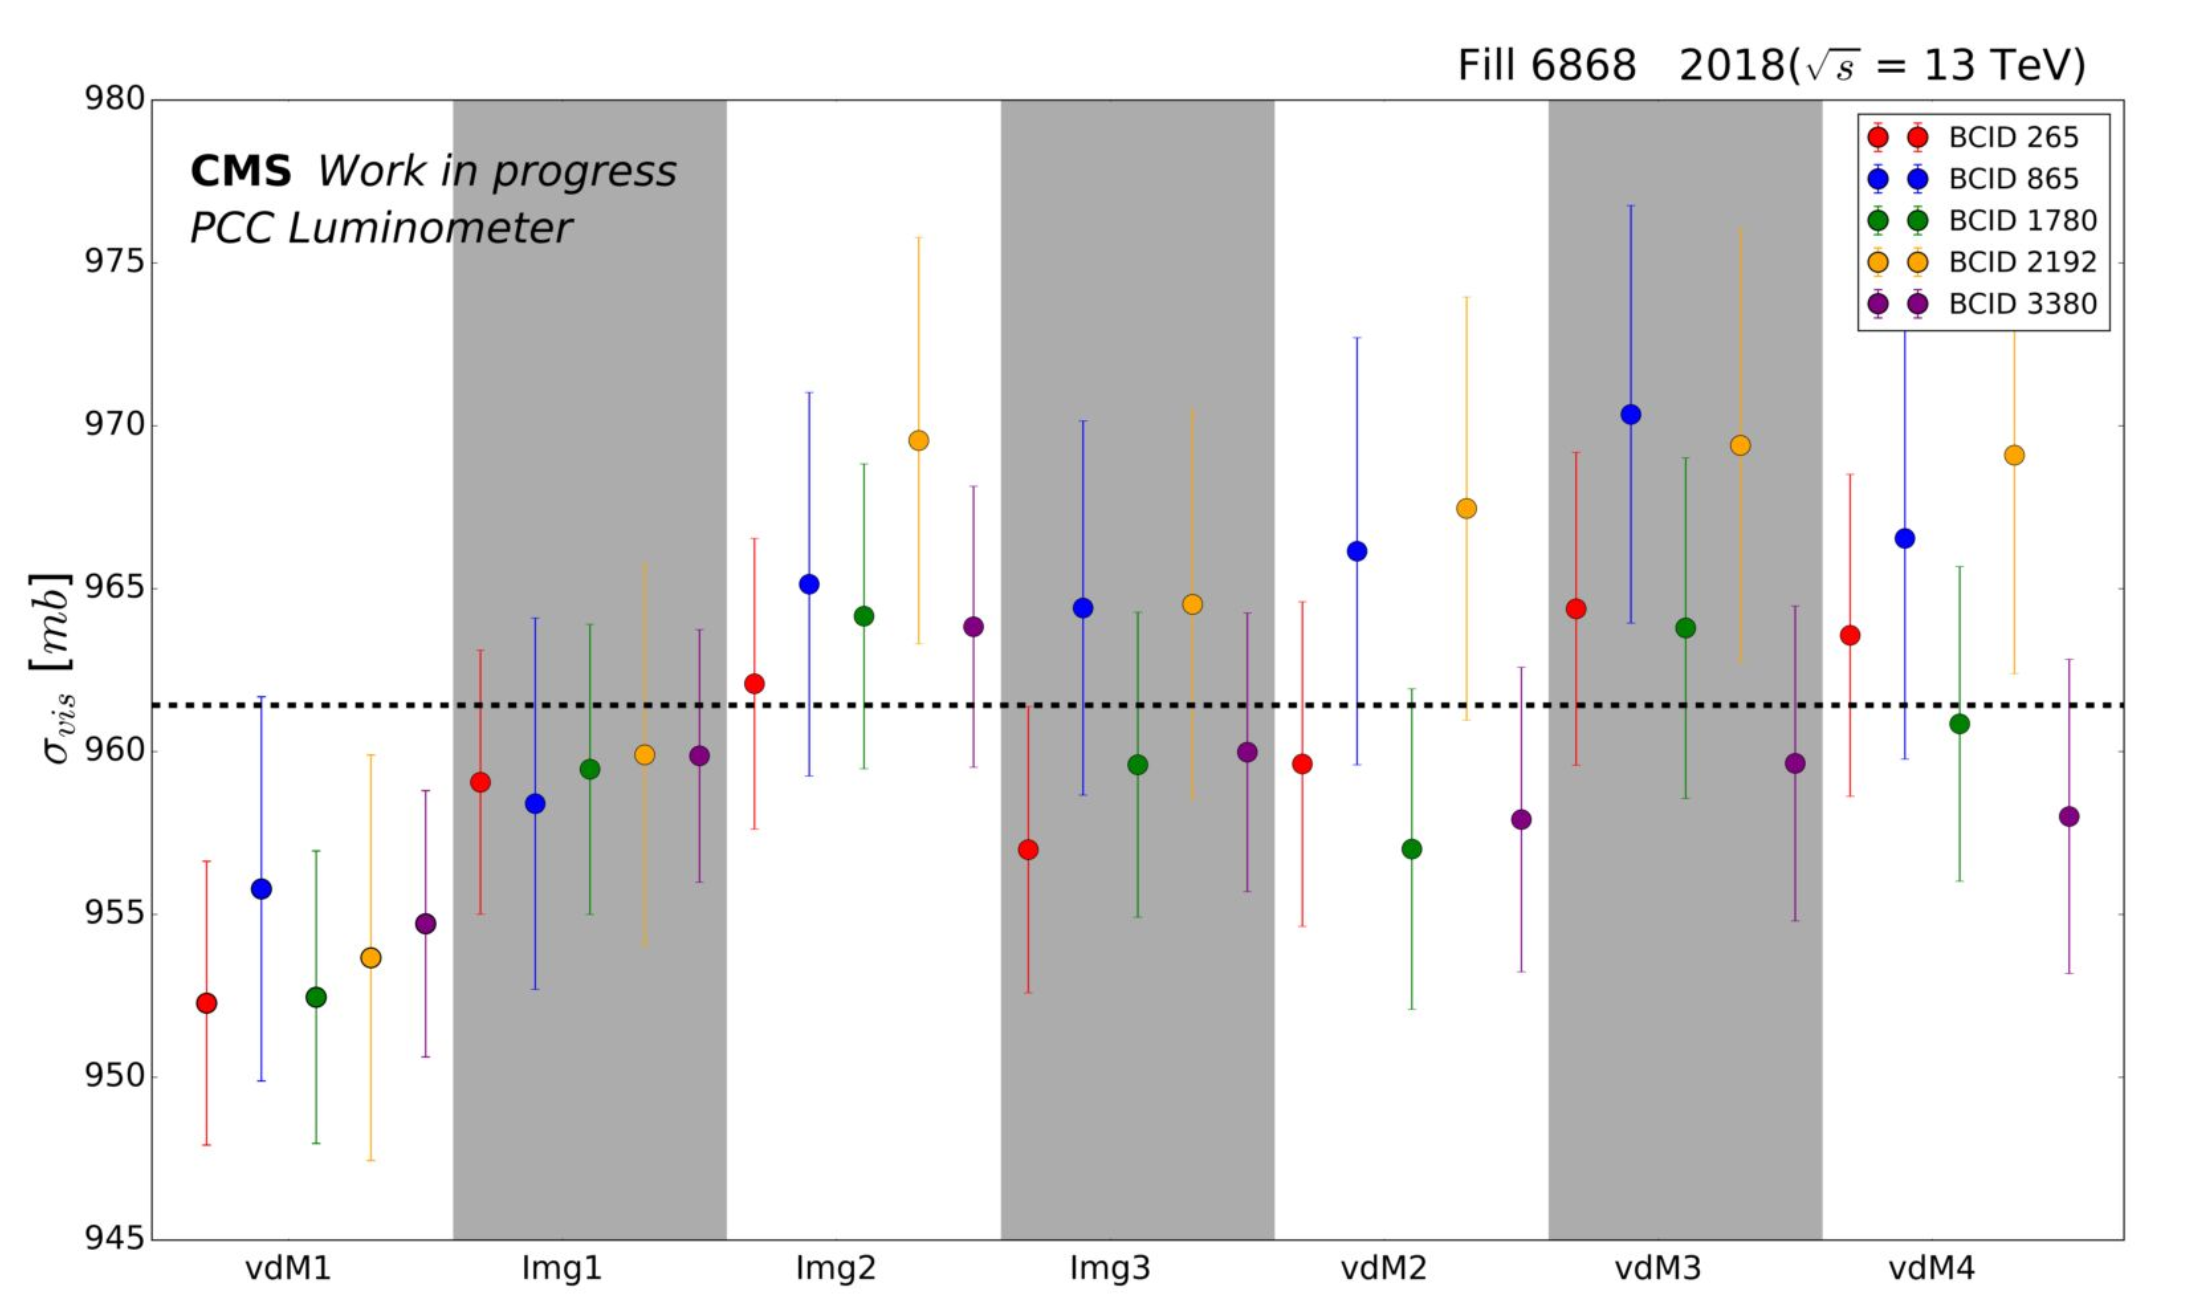
\includegraphics[width=0.7\textwidth]{ashish_thesis/sigma_vis_btob_var_1.png}
\caption[$\sigma_{vis}$ Bunch Variation]{%                                                                                                                                                       
 Bunch to bunch variation of PCC visible cross section.
}
\label{fig:sigmavis_btob_variation}
\end{figure}

\newpage
\section{Luminosity for physics fill}

The LHC operates in cycles known as "fills." A fill is a period during which the LHC is filled with protons and provides collisions for its experiments. The luminosity profile of a fill is a graphical representation of the instantaneous luminosity as a function of time for the entire duration of that fill. Before the actual data taking begins, there is a phase of beam injection, acceleration, and stabilization. During this period, no collisions are taking place, so the luminosity is zero. Once the beams are accelerated to their maximum energy and brought into collision, there is a rapid rise in luminosity. This is the point where the luminosity reaches its highest value, known as the peak luminosity. After the peak, the luminosity starts to decrease. This period, known as "stable beams", is when most of the data is collected. The reason for the decrease in luminosity over time is the reduction in the number of protons in the beams due to collisions. As the protons in the beams collide, the number of protons, and hence the luminosity, diminishes. The rate of this decrease can be influenced by various factors, including beam dynamics, losses, and the efficiency of the collider's operation. The fill concludes when the number of protons is too low to provide useful data, or if there's a technical issue, leading to a beam dump. At this point, the luminosity drops to zero. The total duration of a fill can vary. Some fills last only a few hours, while others can extend for over a day, depending on operational efficiency and the goals for that specific fill. Fill profile for Fill 6961 during 2018 data taking is shown in Fig. \ref{fig:Fill6961} with

\begin{itemize}
  
\item Peak luminosity = $1.85 \times 10^{34} cm^{-2} s^{-1}$
\item End luminosity = $0.9 \times 10^{34} cm^{-2} s^{-1}$ 
\item Number of colliding bunches = 2556
\item Number of lumi sections = 1400
\item Integrated luminosity = 0.418 $fb^{-1}$

\end{itemize}
    
\begin{figure}[!htp]
    \centering
    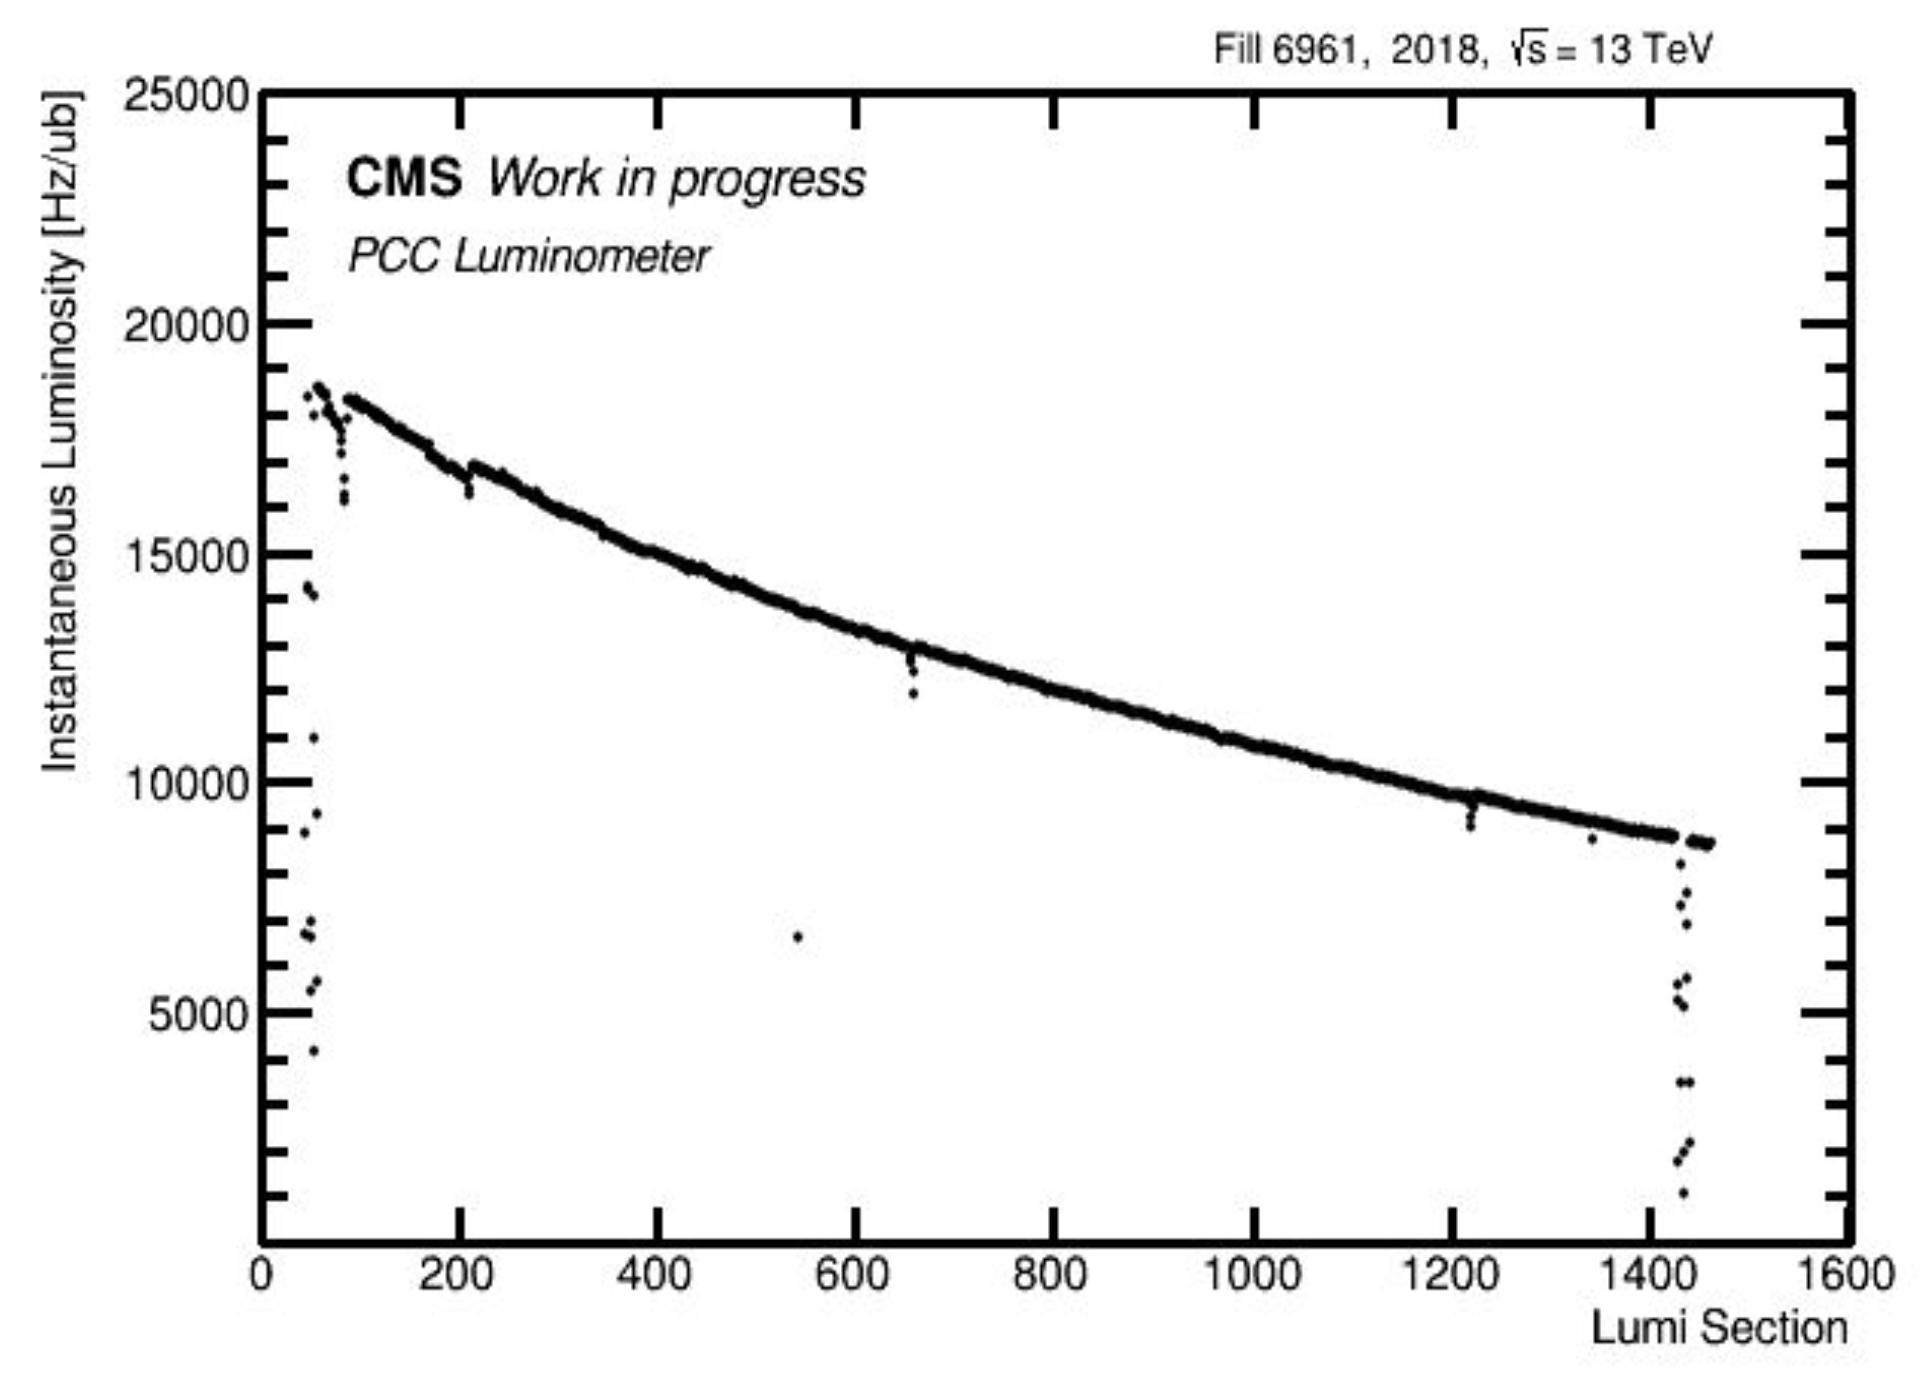
\includegraphics[width=0.9\textwidth]{ashish_thesis/Fill_profile_6961_1.png}
    \caption[Fill 6961 Profile]{Typical lumi profile for LHC Fill during 2018 data taking period for Fill 6961.}
    \label{fig:Fill6961}
\end{figure}


\newpage
\subsection{Afterglow backgrounds}

In the precision PCC luminosity measurement, understanding and rectifying the effects of afterglow is crucial. When estimating afterglow corrections, it's paramount to utilize raw PCC data obtained from both colliding and non-colliding bunches. The colliding bunches yield genuine signals representative of particle interactions, while the non-colliding bunches illuminate the background noise inherent in the system, simultaneously capturing any lingering afterglow from prior collisions. Two primary types of afterglow noise have been identified:

Type 1 Afterglow (Electronic Spillover): This noise arises due to the lingering signal waveform in silicon after an actual collision event.

Type 2 Afterglow (Activation-Induced Background): This noise is a consequence of the gradually diminishing activation of the detector. It occurs when the detector material encounters high-energy particles, leading to the creation and decay of radioactive isotopes \cite{CMS-PAS-SMP-12-008} %(as depicted in Fig. \ref{fig:pcc_afterglow}).

The afterglow correction process seeks to adjust for these residual signals, which result in background added to the cluster count. The concept of 'afterglow' is intrinsically tied to the detector and the events it records, independent of the specific modules used for data collection. Thus, regardless of any module's performance or operational state, the need for consistent afterglow correction remains.

In the afterglow correction process, following steps are involved.

\begin{itemize}
\item A model is constructed to mirror the afterglow tail from a single colliding bunch using the random trigger data.
\item The model is then fine-tuned according to the luminosity associated with that bunch.
\item In the ongoing correction process, a histogram representing the collision events and containing bunch trains is adjusted whereby the afterglow model, multiplied by the luminosity of each colliding pair, is subtracted from all subsequent collision events. This step ensures each bunch is comprehensively corrected.
\item Finally, the scale factor for correction is defined by the ratio of the corrected to the uncorrected PCC. This factor is then implemented in the final PCC for the ZB data. %An example plot of the scale factor is shown in Fig. \ref{fig:af_change_veto}.
\end{itemize}

Moreover, pedestal correction is essential. It signifies the adjustment of baseline values in the detector due to electronics noise. This procedure ensures accurate and stable readings from the pixel detector, culminating in precision PCC luminosity measurements. %An example of the afterglow correction factor including type 1, type 2 and pedestal corrections is shown in Fig. \ref{fig:af_change_veto}. 

For accurately modeling the afterglow effect in raw data, a composite function is utilized. It includes parameters for the Type 1 afterglow and an exponentially decaying model for Type 2, taking both amplitude and decay width into account. The model is summed over all bunch crossings.

\begin{equation}
F(x) = \sum_{k=0}^{N_{\text{bcid}}} N_k \left[ (x - k == 0) + A  (x - k == 1) + B  \exp(-C  (x - k - 1))  (x - k \geq 1) \right]
\end{equation}

Fill 9036, shown in \ref{fig:af_fit40} and encompassing 900 colliding bunches, serves as the foundation for estimating the Type 2 afterglow parameters. A fit is performed to one wagon train, then two, and finally three, refining the parameters for Type 2 afterglow and minimizing the residuals of both afterglow types. Fit plots for single train is shown in \ref{fig:af_fit99}. The values of type 2 afterglow parameter amplitude (B) and decay width (C) for different wagon trains are shown in Table \ref{fig:af_fit4000}. 

\begin{comment}

Type 1 and Type 2 afterglow corrections are very important for precise PCC luminosity measurement. Type 1 afterglow noise, or electronic spillover, arises due to the lingering signal waveform within silicon after actual collision event. Contrarily, Type 2 afterglow noise emanates from the exponentially diminishing activation of the detector caused by the creation of secondary particles when the detector material encounters high-energy particles \cite{CMS-PAS-SMP-12-008} (as depicted in Fig. \ref{fig:pcc_afterglow}).

The rectification of afterglow noise is achieved by constructing a model that replicates the tail of the afterglow from a single collision event. This model is then adjusted according to the luminosity of the event. In an ongoing process of correction, a histogram representing the collision events and containing bunch trains is adjusted, whereby the afterglow model is multiplied by the luminosity of each colliding pair and subsequently deducted from all subsequent collision events. This iterative process is repeated for all colliding pairs, ensuring each event is completely rectified prior to being used for further correction.

The afterglow correction, or the scale factor, is determined by calculating the ratio of the corrected to uncorrected PCC. This factor is then implemented into individual event histograms within the zero bias data.

%The afterglow correction is independent of the module veto list as shown in Fig. \ref{fig:af_change_veto} , meaning the correction is applied universally across all modules irrespective of whether a module is on the veto list or not. This is because afterglow is a characteristic of the detector material and particle interactions, not of the specific modules. Thus, even when the module veto list changes, the afterglow corrections remain consistent, ensuring accurate luminosity measurement.

The afterglow correction in PCC luminosity measurement is a compensatory procedure that's designed to adjust for the lingering effects of prior particle collisions, which may otherwise skew the accuracy of the luminosity calculations. The concept of 'afterglow' is related to these residual signals, identified as Type 1 and Type 2, that originate from the detector material and the physical processes associated with the particle interactions. Importantly, the presence and extent of afterglow are influenced by these fundamental factors and are not dictated by the operational state or quality of any individual detector module as shown in Fig. \ref{fig:af_change_veto}. That is, the afterglow is an inherent characteristic tied to the detector and the physical event, and it is independent of the specific modules being used to collect the data. A module veto list is a register of detector modules that are excluded from data collection and analysis for various reasons, such as suboptimal performance, high noise levels, or other technical issues. When a module is added to or removed from the veto list, it can affect the raw data that's being gathered, but it doesn't influence the underlying afterglow characteristics that are tied to the detector material and the particle collisions. Therefore, changes to the veto list do not alter the need for, or the application of, the afterglow correction. Consequently, the afterglow correction process remains consistent and is applied across all modules, irrespective of their veto list status. This ensures that the measured luminosity accurately represents the actual particle collision events, providing reliable data for subsequent analysis and interpretation, regardless of the specific module configuration at any given time.

Apart from afterglow corrections, pedestal correction is another critical component. It signifies the adjustment of baseline values in the detector readout to account for any systematic biases or drifts. The pedestal correction involves monitoring the detector's output in the absence of a signal, and then subtracting this baseline value from the signal collected during data capture. The application of pedestal correction significantly enhances the accuracy and stability of the pixel detector's readings, thereby leading to precision measurement of PCC luminosity.

\newpage
\begin{figure}[H]
\centering
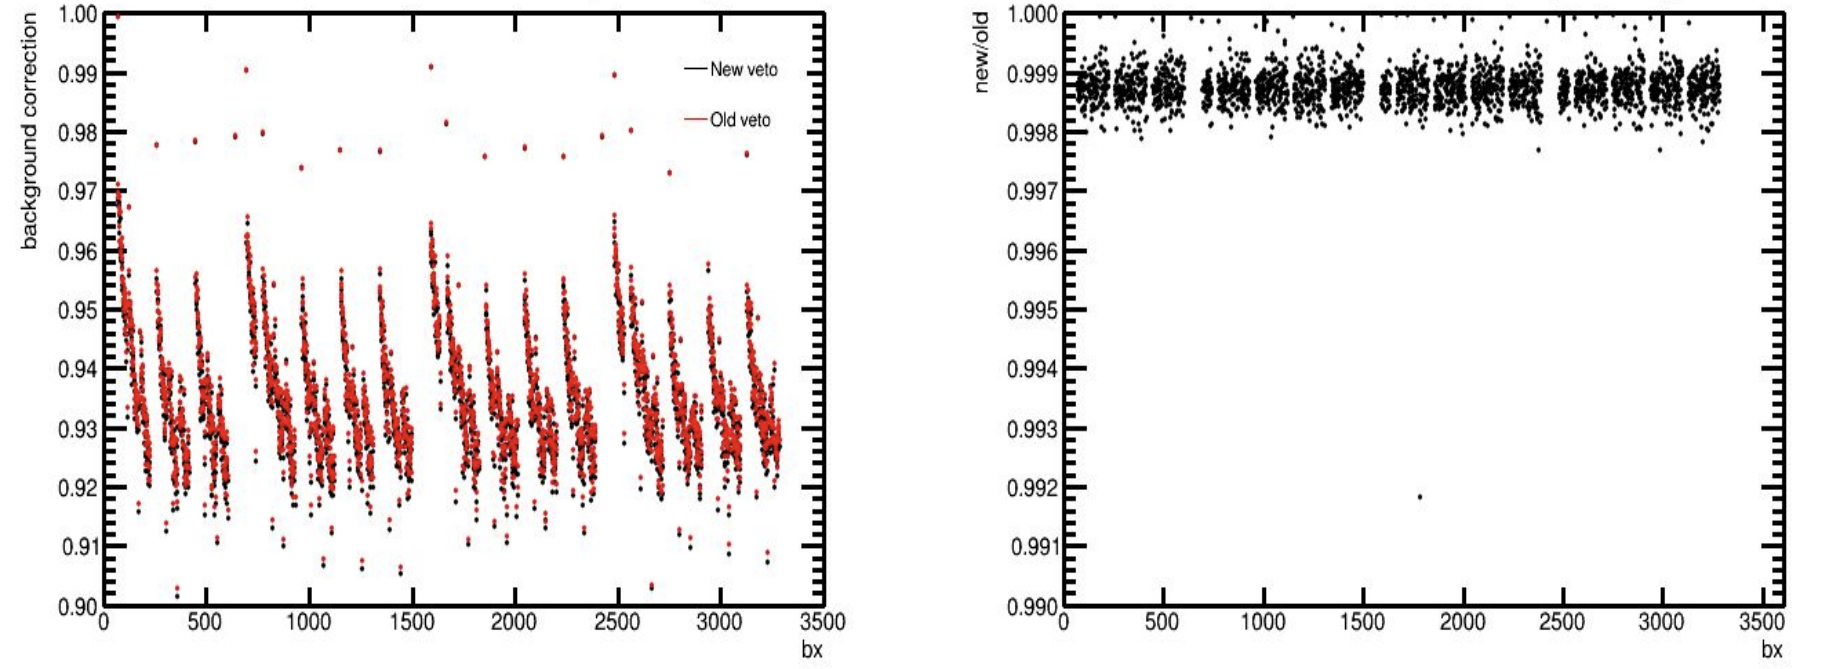
\includegraphics[width=0.7\textwidth]{ashish_thesis/veto_change_same_af.png}
\caption[Afterglow background ratio]{%                                                                                                                                                                         
    Ratio of afterglow scale factor for new per period veto and old veto.
}
\label{fig:af_change_veto}
\end{figure}

%Type 1 and Type 2 afterglow corrections are essential for obtaining accurate PCC measurements. Type 1 afterglow noise, also known as electronic spillover, is caused by the long waveform of the signal in silicon. On the other hand, Type 2 afterglow noise is the exponentially decaying detector activation due to the production of secondary particles when high-energy particles interact with the detector material as shown in Fig. \ref{fig:pcc_afterglow}. Afterglow noise is corrected by creating a model of the afterglow tail of a single colliding bunch, which is then normalized to the luminosity of the colliding bunch crossing. A bunch-by-bunch histogram containing bunch trains undergoes afterglow correction, where the afterglow model is multiplied with the luminosity of each colliding bunch pair and subsequently subtracted from all following bunches. This correction process is performed iteratively for all colliding bunch pairs, ensuring that a given bunch crossing is fully corrected before being used to correct the subsequent bunch crossings. The afterglow correction, or scale factor, is calculated by taking the ratio of the corrected and uncorrected PCC. This scale factor is then applied to individual bunch-by-bunch histograms in the zero bias data. In addition to afterglow corrections, pedestal correction is another important aspect to consider. Pedestal correction refers to the adjustment of baseline values in the detector readout to account for any systematic offsets or drifts. This process involves measuring the detector's output when no signal is present and subtracting this baseline value from the measured signal during data collection. By performing pedestal correction, the accuracy and stability of the detector's measurements are significantly improved, contributing to more reliable PCC measurements.

%Type 1 and 2 afterglow corrections are measured and applied to the PCC measurement. Type 1 afterglow noise is electronic spillover due to long waveform of the signal 549 in silicon and Type 2 afterglow noise is exponentially decaying detector activation due to production of secondary particles when high energy particles interact with detector material as shown in Fig. 15. Afterglow noise is corrected by making a model of afterglow tail of a single colliding bunch, normalized to the luminosity of the colliding bunch crossing. Bunch-by-bunch histogram containing bunch trains is corrected for afterglow where afterglow models is multi554 plied with the luminosity of each colliding bunch pair and subtracted from all following bunches. This correction is performed iteratively over all colliding bunch pairs such that a given bunch crossing is fully corrected before it is used to correct the succeeding bunch crossings. The afterglow correction (or scale factor) can be calculated by taking the ratio of corrected and uncorrected PCC. This scale factor is applied to individual bunch-by-bunch histograms in the zero bias data.

\begin{itemize}

\item Type 1 afterglow correction: Type 1 afterglow refers to the residual signals in the detector caused by particles from previous bunch crossings. These particles can be trapped in the detector's sensitive volume, leading to an overestimation of the actual number of pixel clusters. The Type 1 afterglow correction aims to correct for this by subtracting the expected contribution of these residual signals from the raw PCC data.

\item Type 2 afterglow correction: Type 2 afterglow is associated with the activation of detector material due to high-energy particle interactions. When high-energy particles interact with the detector material, they can cause the material to become radioactive. The decay of these radioactive isotopes produces additional signals in the detector, which can lead to an overestimation of the number of pixel clusters. The Type 2 afterglow correction aims to account for these additional signals by subtracting the expected contribution of the activation-induced background from the raw PCC data.

\item Pedestal correction: The pedestal correction refers to the baseline noise level in the detector, which can be influenced by factors such as temperature fluctuations, electronic noise, and radiation damage. This noise can cause an over- or underestimation of the actual number of pixel clusters. The pedestal afterglow correction aims to correct for this by adjusting the raw PCC data based on a measurement of the pedestal noise level.

\end{itemize}

\end{comment}

%The scale factor for one 50 lumi section block in run number 315690 is shown in Fig. \ref{fig:af_change_veto}. It provides an overview of the afterglow scale factor applied to the raw PCC. On the left, both the raw and corrected PCC for all bunch crossings are displayed, showing the variations between the initial data and the adjusted counts. The right side specifically highlights the afterglow scale factor for a single 50 lumi section block, representing the afterglow correction applied for final module veto. 

%\begin{figure}[!htp]
%\centering
%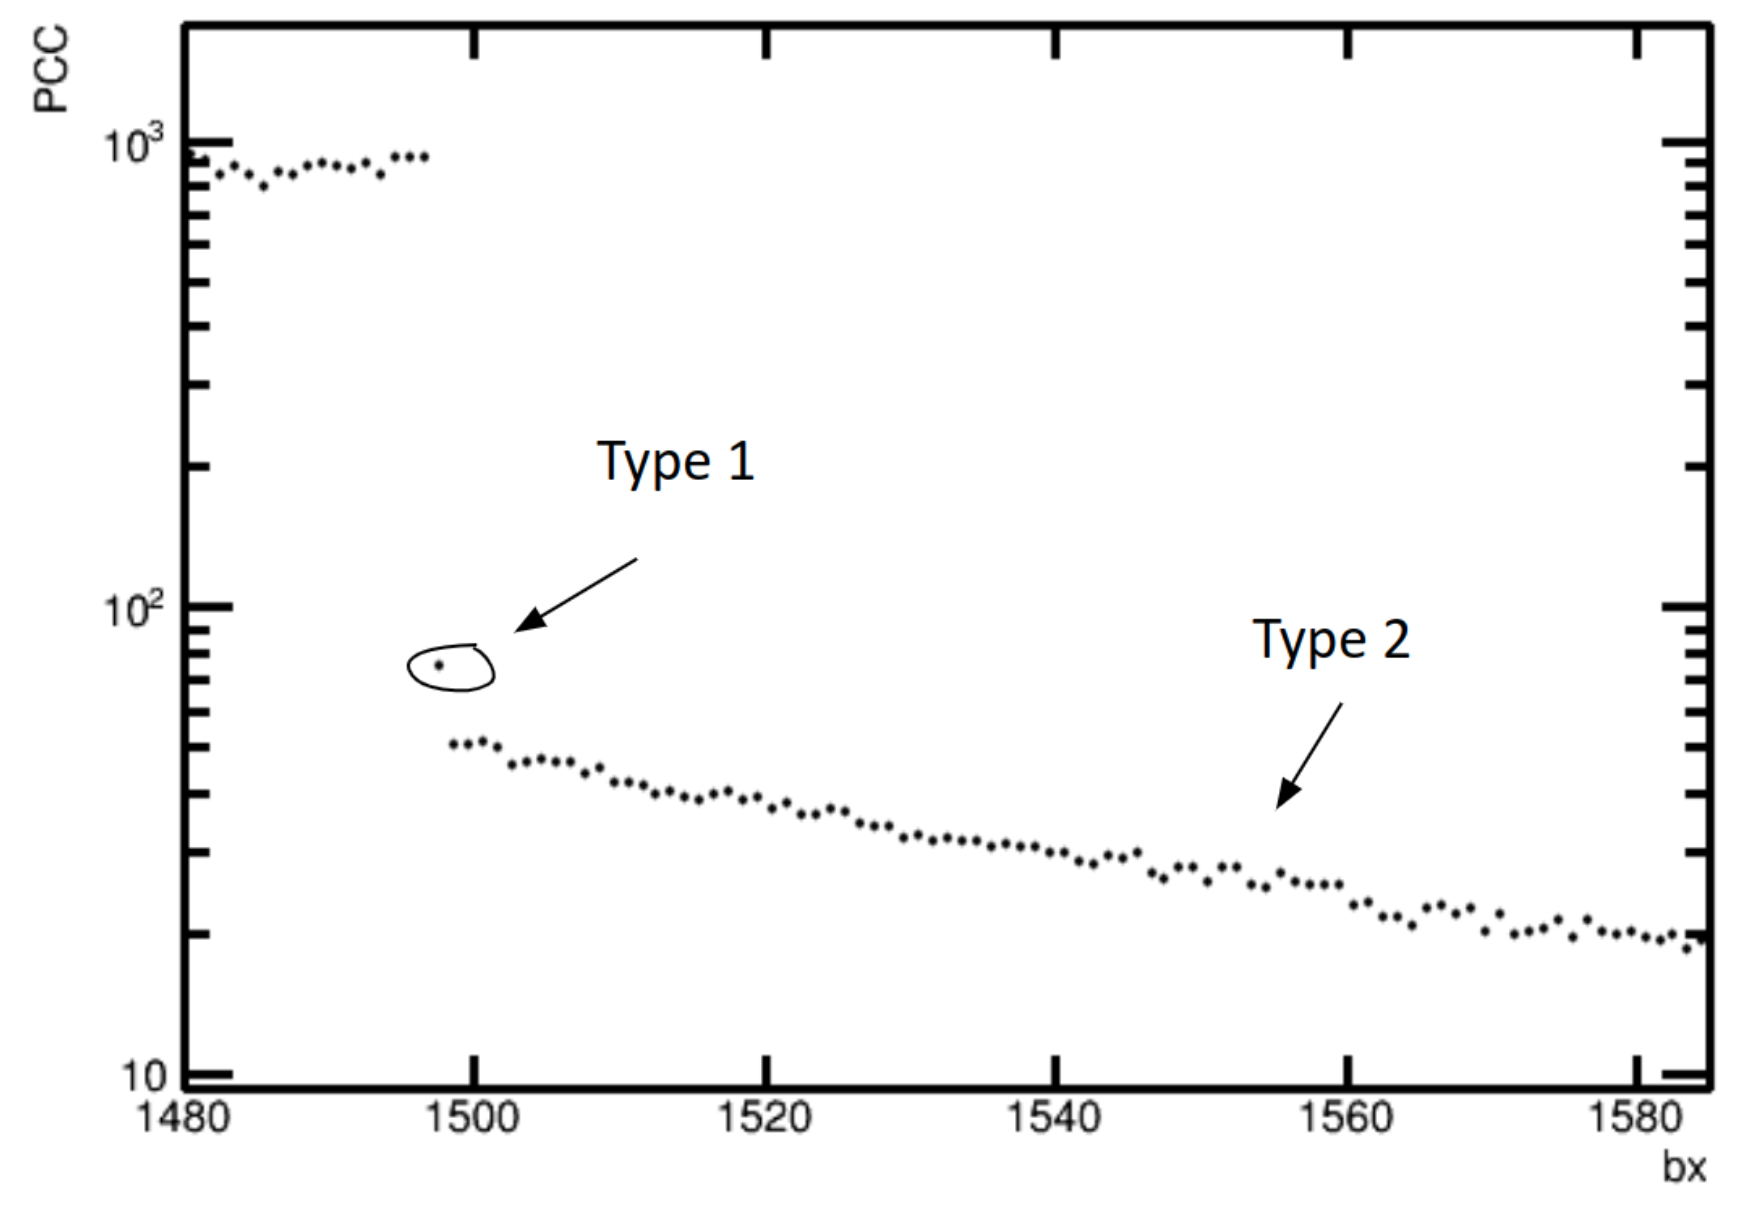
\includegraphics[width=0.7\textwidth]{ashish_thesis/af_t1_t2.png}
%\caption[Afterglow Effect Single Bunch]{%
%Afterglow corrections are calculated from cluster rate measurements in empty bunches. Electronic spillover (“Type-1”). Type-1 noise is due to long waveform of the signal in silicon. First empty bunch after bunch train is used to calculate it. Exponentially decaying detector activation (“Type-2”).  Type-2 noise is due to production of secondary particles when high energy particles interact with detector material. All empty bunches after bunch train are used to calculate it.
%}
%\label{fig:pcc_afterglow}
%\end{figure}


%\begin{figure}[!htp]
%\centering
%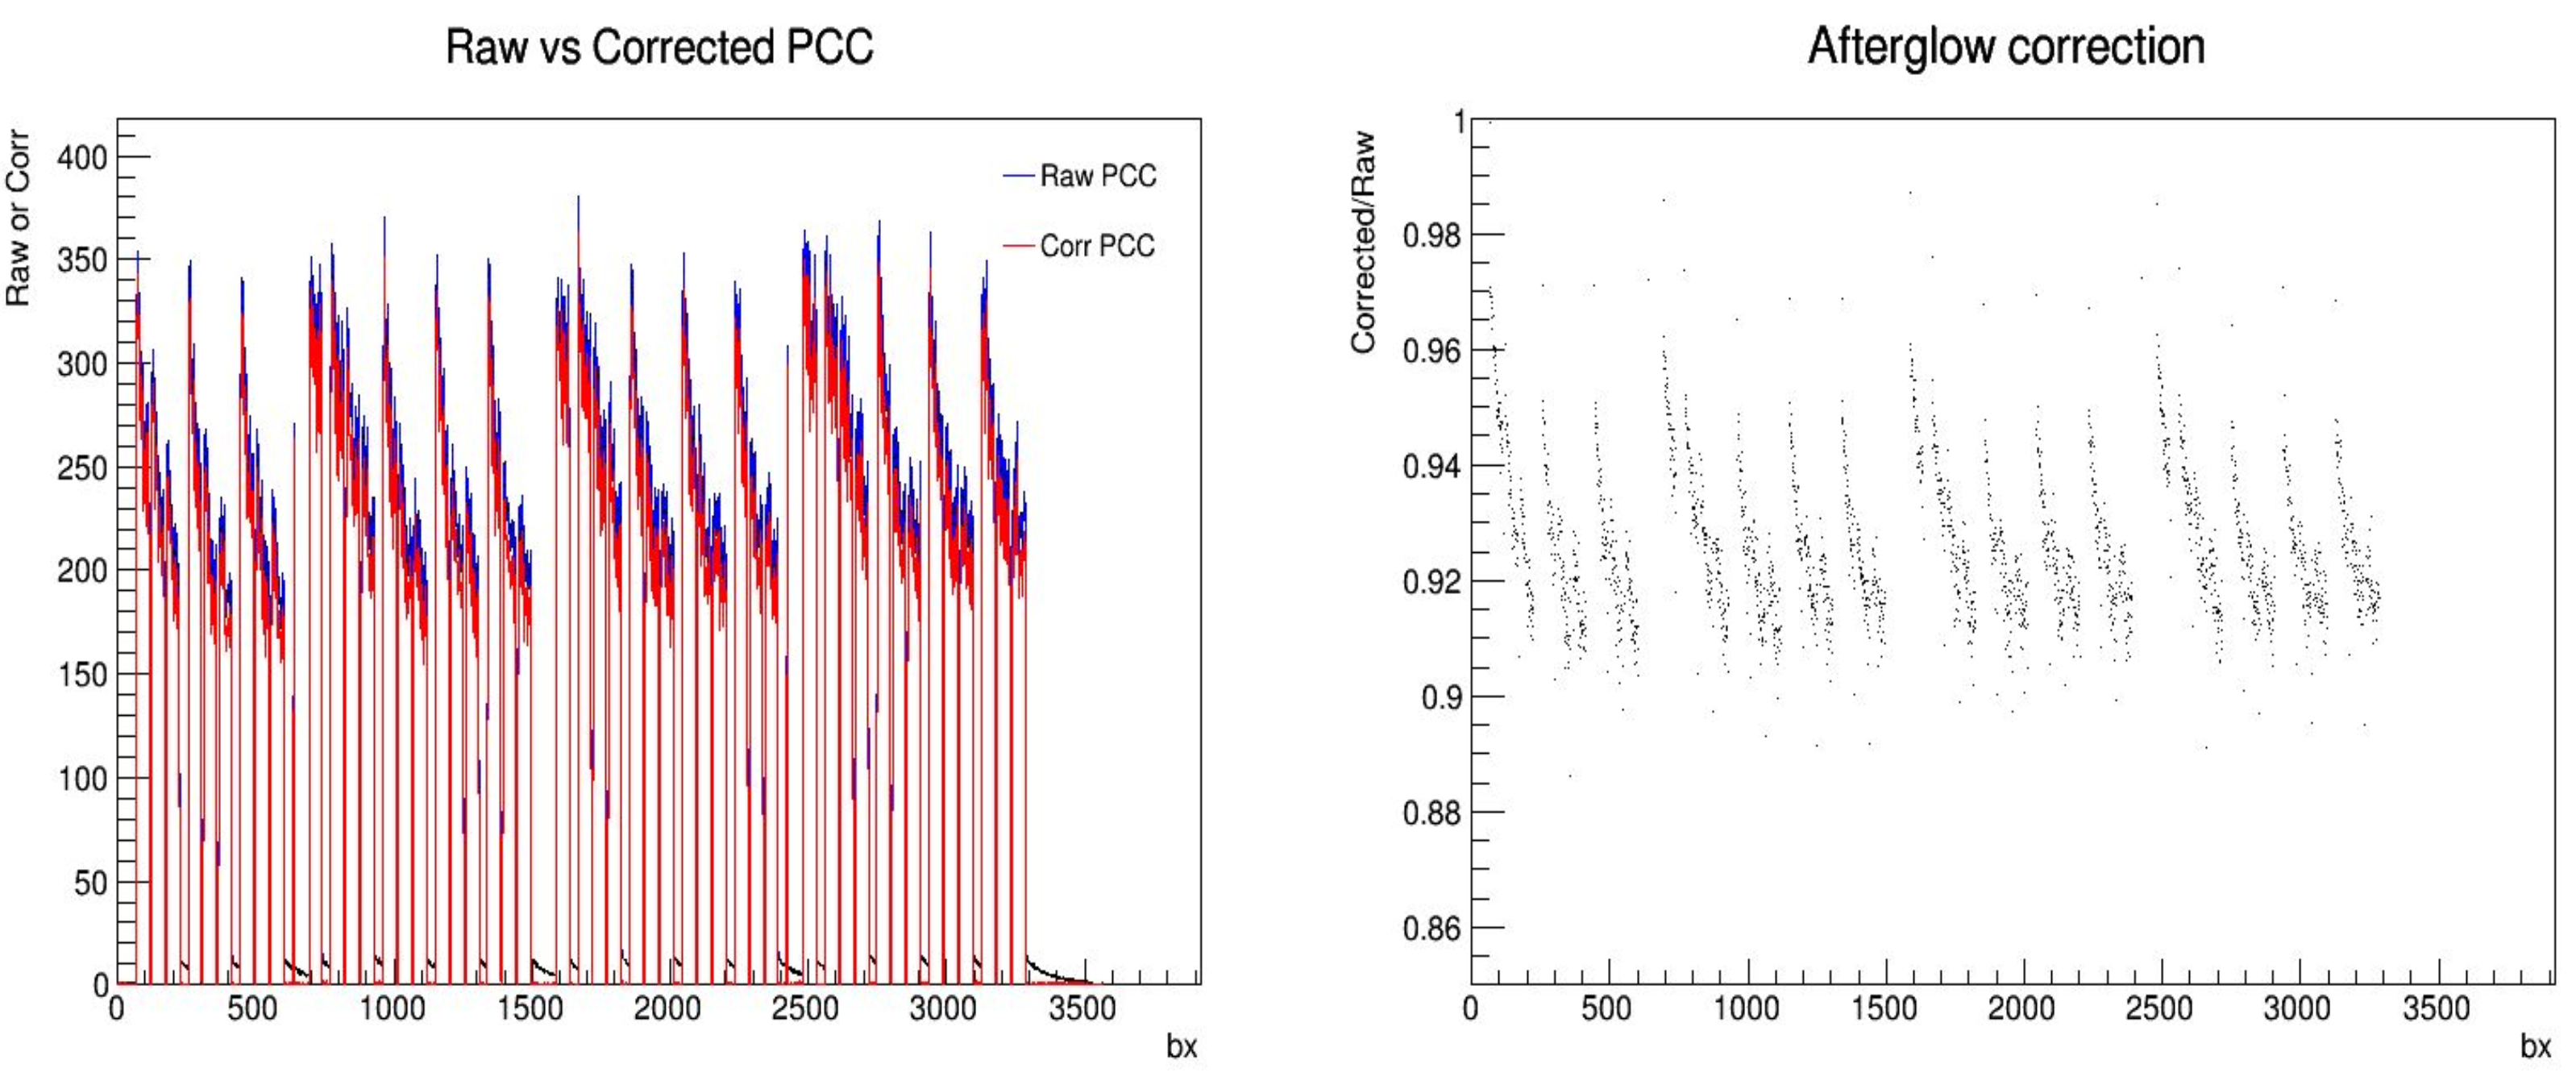
\includegraphics[width=1\textwidth]{ashish_thesis/afterglow_correction_factor_1lsblock_315690.png}
%\caption[Afterglow background]{%                                                                                                                                                                                          
% Left: Raw and corrected PCC for all bunch crossings. Right: Afterglow scale factor for one 50 lumi section block in run 315690 for the final module veto.
%}
%\label{fig:af_change_veto}
%\end{figure}

\begin{comment}

The model used for fitting the afterglow in PCC raw data consists of a parameter for type 1 afterglow correction and exponentially decaying model with two parameters for type 2 afterglow correction taking into account amplitude and decay width. The fit function is summed over all bunch crossings. Fill 9036 (shown in Fig. \ref{fig:af_fit40}) consisting of 900 colliding bunches is used for the estimation of type 2 afterglow parameters. We start by fitting a single 50 lumi section block, then fit one wagon train, two wagon train and three wagon train to get better estimation of type 2 afterglow parameters to obtain least type 1 and type 2 afterglow residuals. 

\end{comment}

\newpage
\begin{figure}[H]
\centering
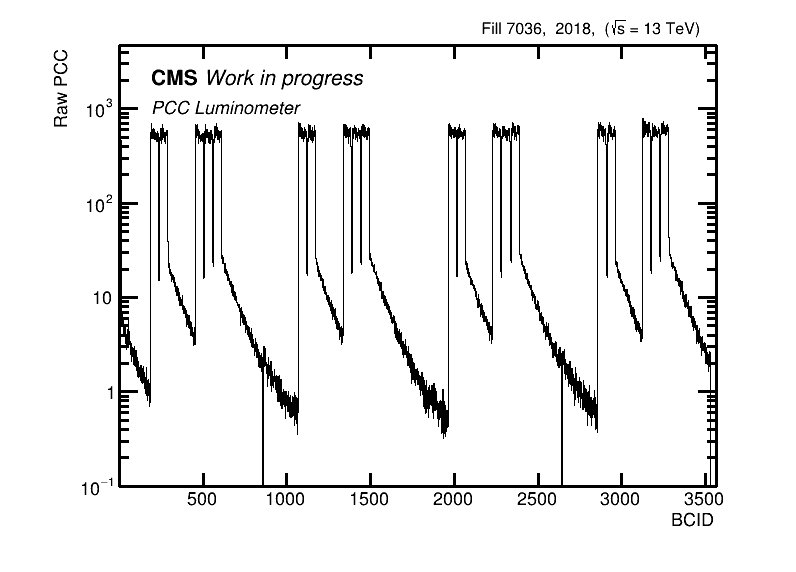
\includegraphics[width=0.8\textwidth]{ashish_thesis/fill_7036_pattern_2.png}
\caption[7036 Fill Patern]{%                                                                                                                                                                                         
  Fill 7036 pattern (900 b fill).
}
\label{fig:af_fit40}
\end{figure}

%Fit plots for single 50 lumi section block, 2 wagon and 3 wagon trains are shown in Fig. \ref{fig:af_fit41}, \ref{fig:af_fit} and \ref{fig:af_fit99}.



%\begin{figure}[!htp]
%\centering
%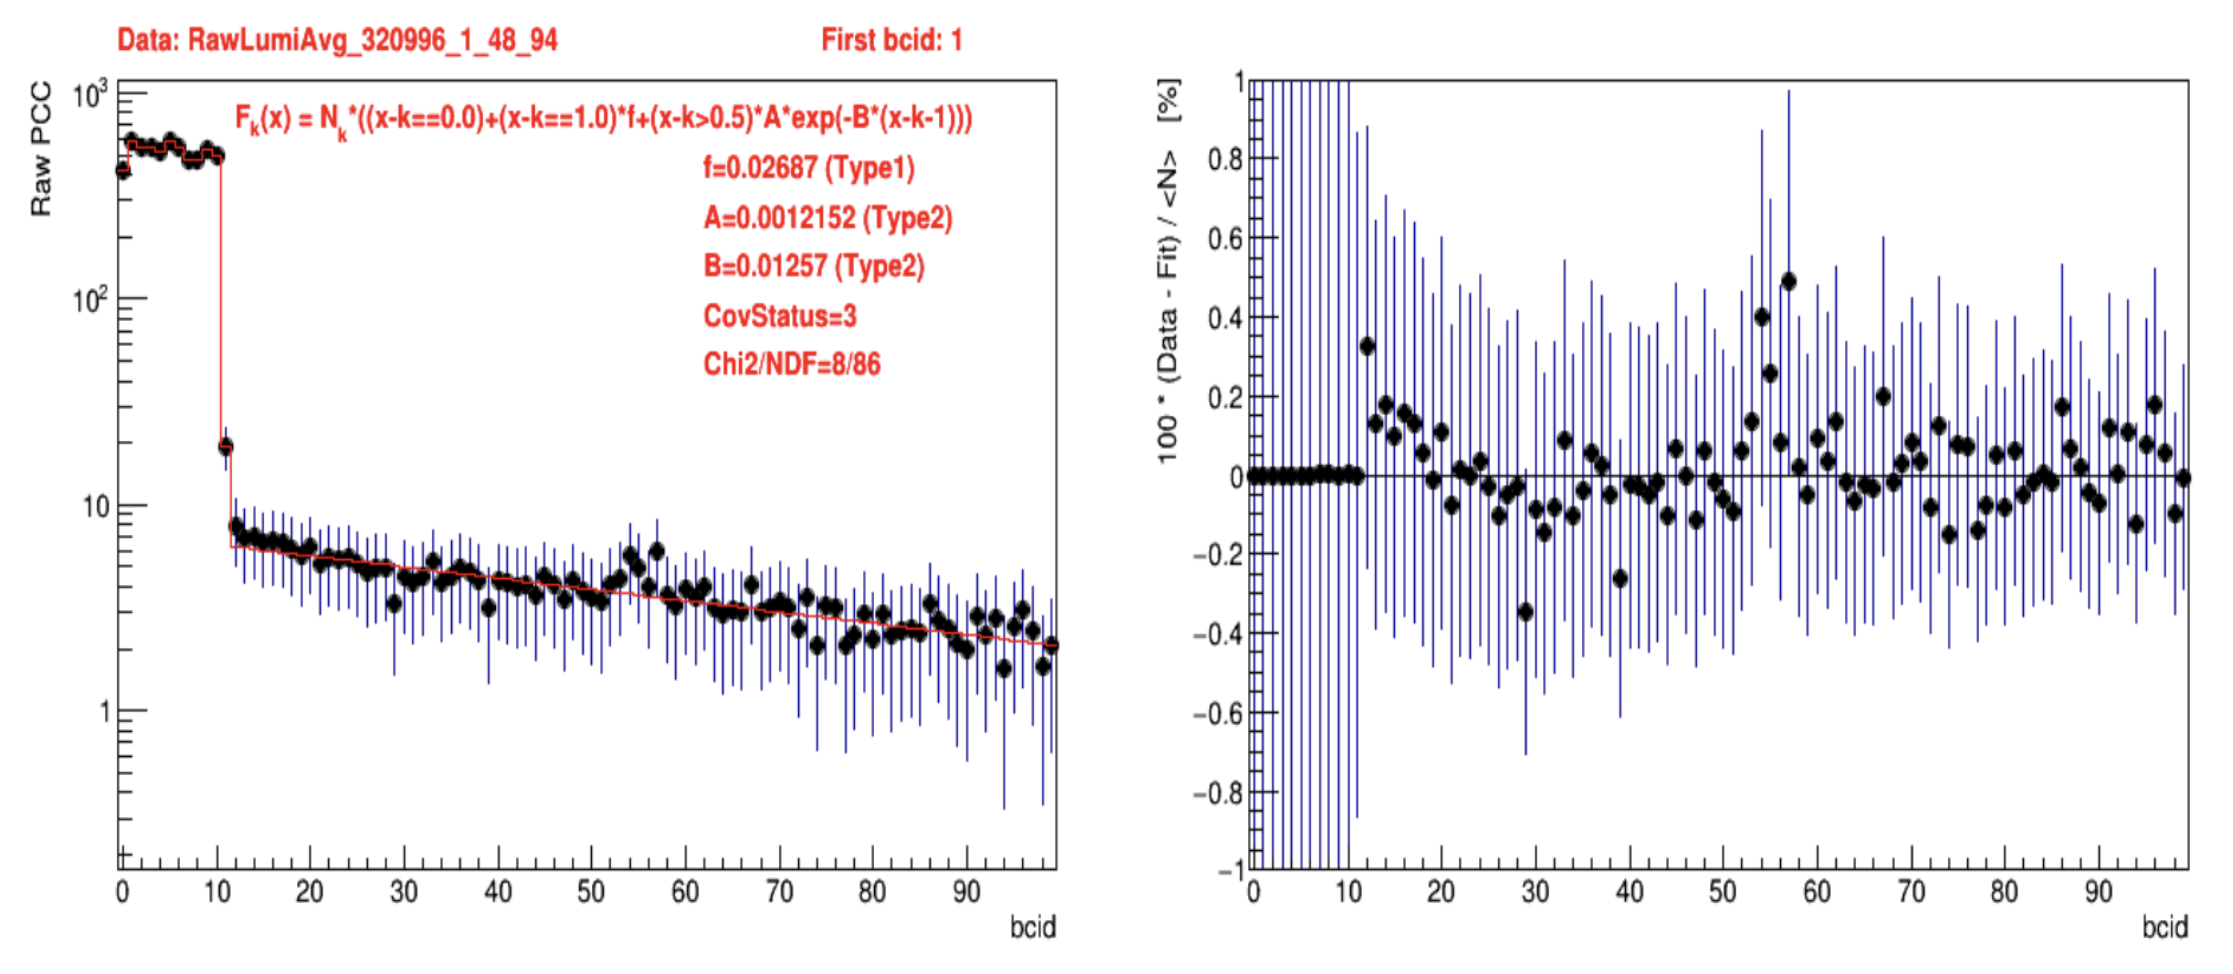
\includegraphics[width=1\textwidth]{ashish_thesis/af_model_fit.png}
%\caption[]{%                                                                                                                                                                                                         
 % Afterglow fit model for single 50 lumi section block.
%}
%\label{fig:af_fit41}
%\end{figure}


%\begin{figure}[!htp]
%\centering
%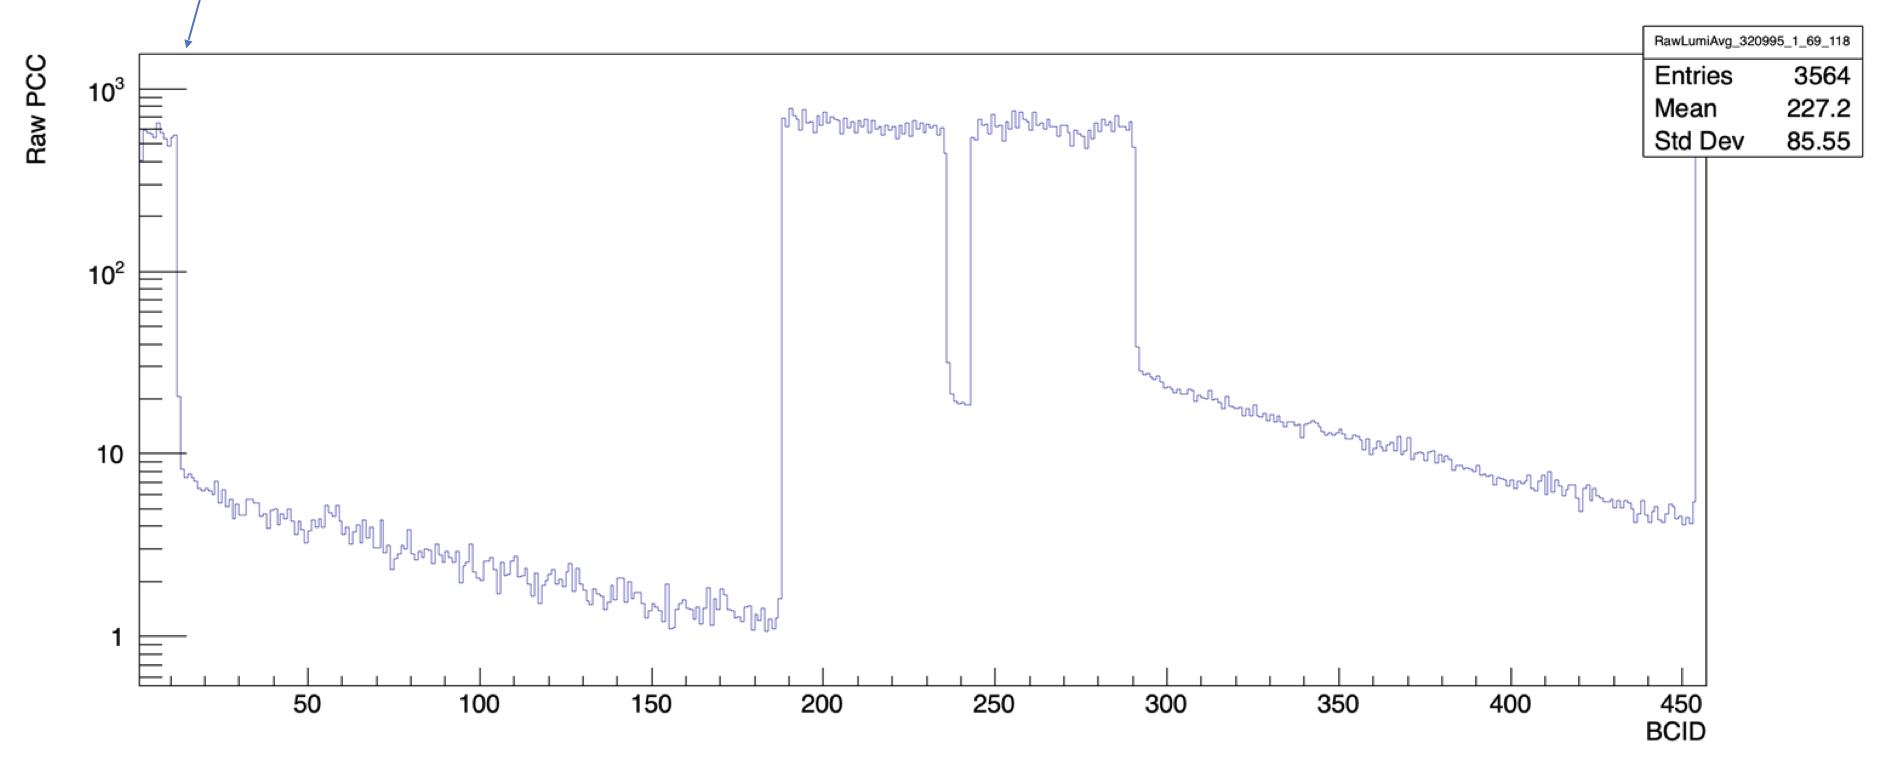
\includegraphics[width=1\textwidth]{ashish_thesis/bunch_train.png}
%\caption[]{%                                                                                                                                                                                  
                                                                                                                                                                                       
  %Afterglow fit model.
%}
%\label{fig:af_fit}
%\end{figure}



%\begin{figure}[!htp]
%\centering
%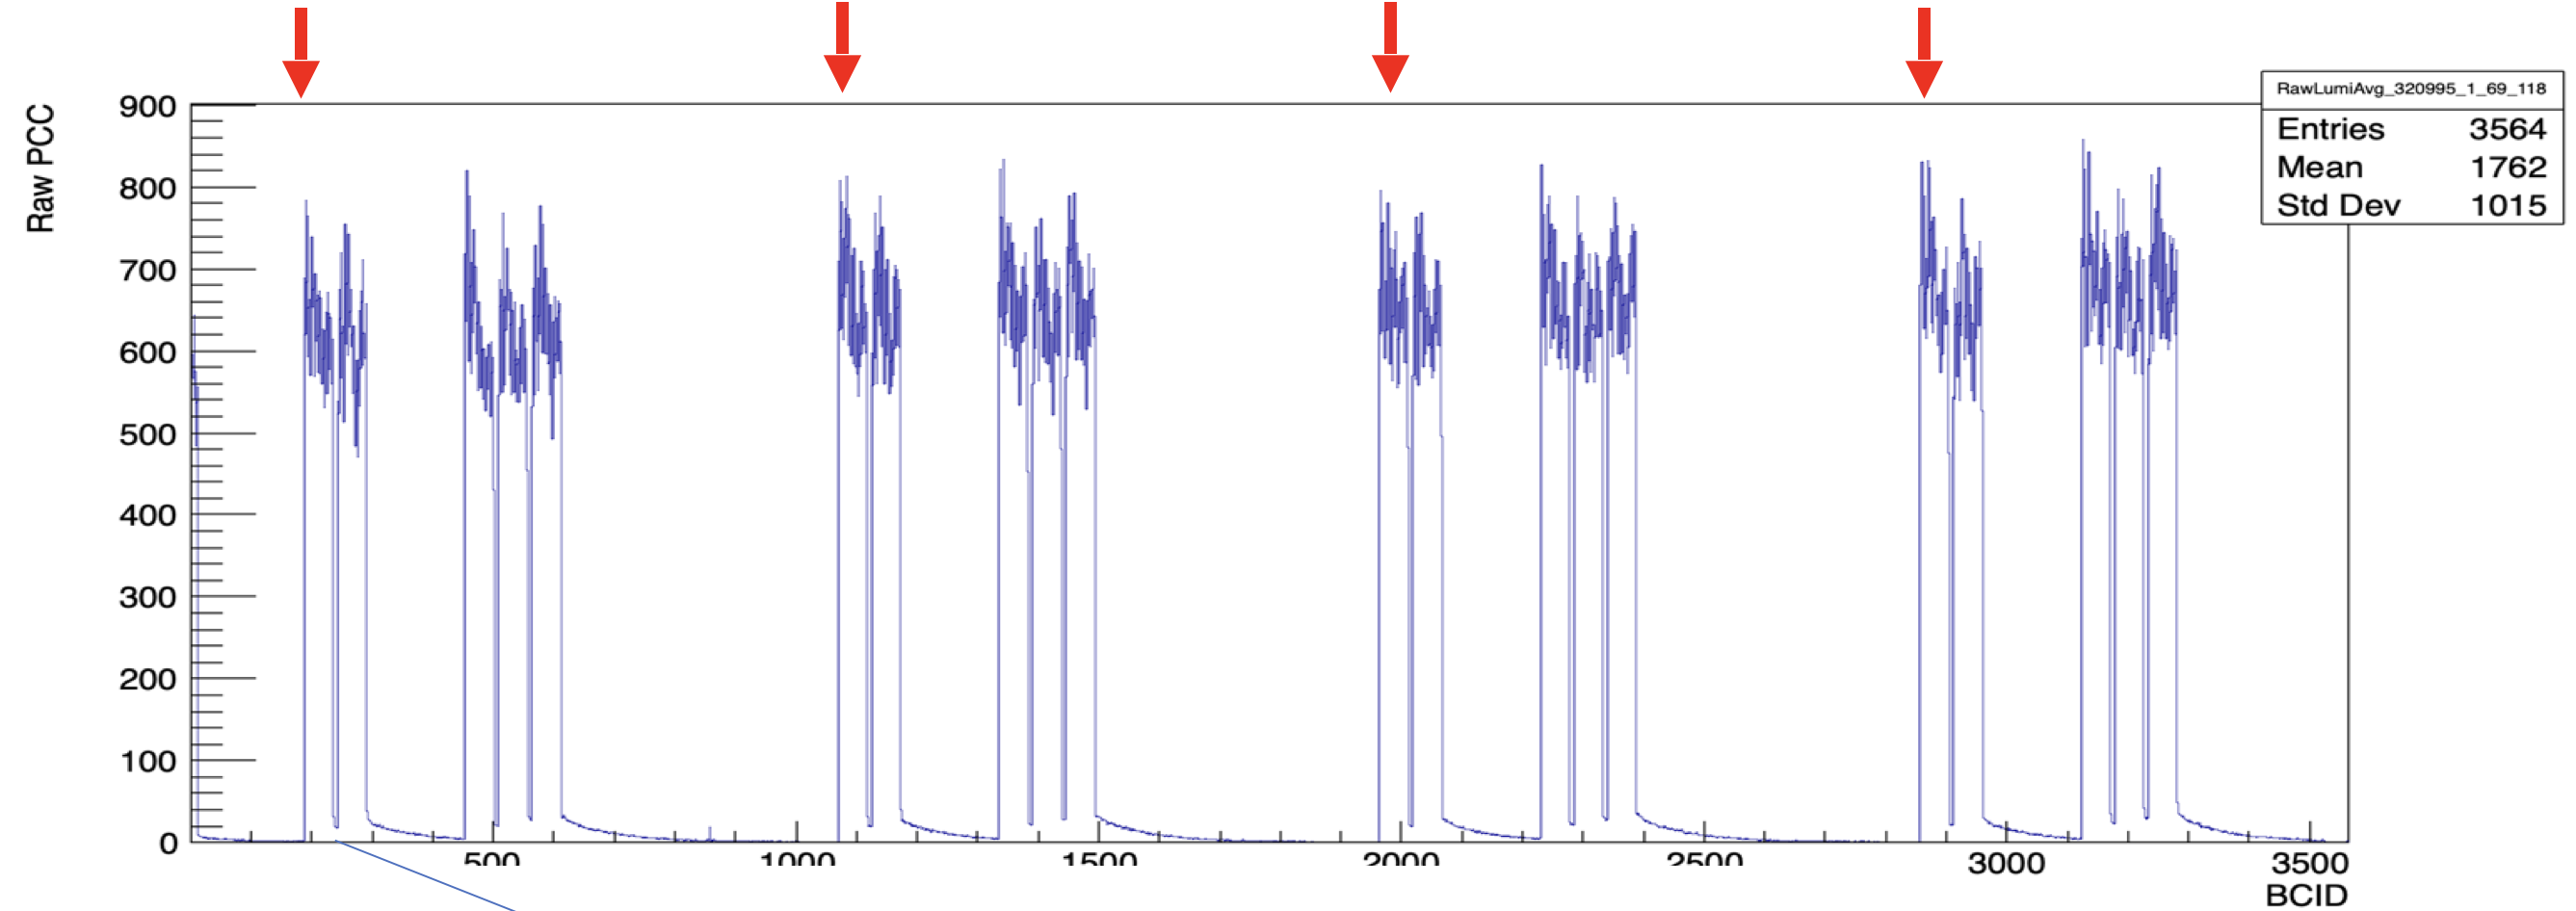
\includegraphics[width=1\textwidth]{ashish_thesis/2wagon_af.png}
%\caption[]{%                                               
                                                                                                                                   
 % Afterglow fit model.
%}
%\label{fig:af_fit}
%\end{figure}

%\begin{figure}[!htp]
%\centering
%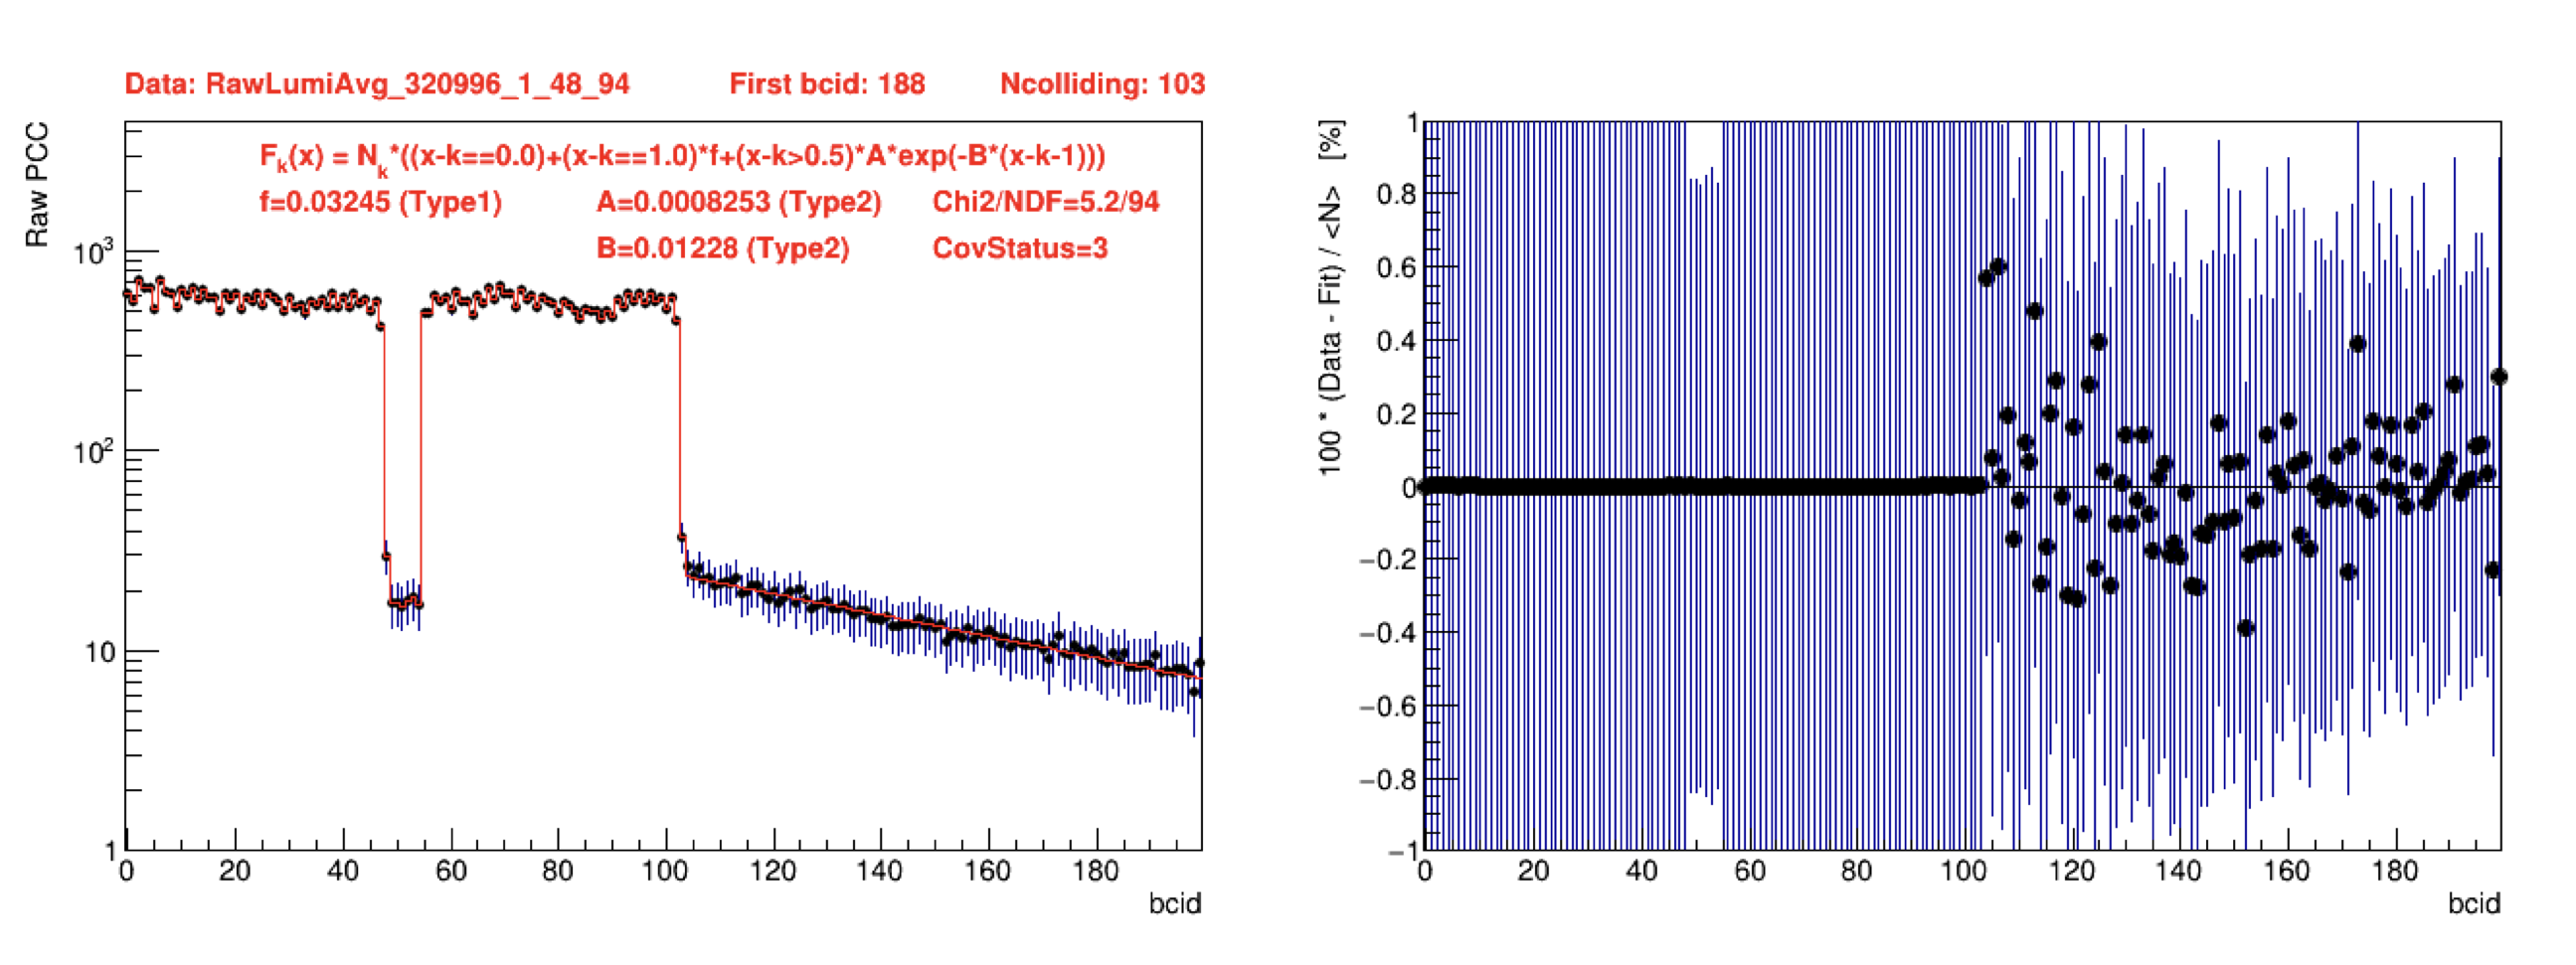
\includegraphics[width=1\textwidth]{ashish_thesis/2wagon_fit.png}
%\caption[]{%                                                                                                                                 
 % Afterglow fit model for 2 wagon train.
%}
%\label{fig:af_fit}
%\end{figure}


%\begin{figure}[!htp]
%\centering
%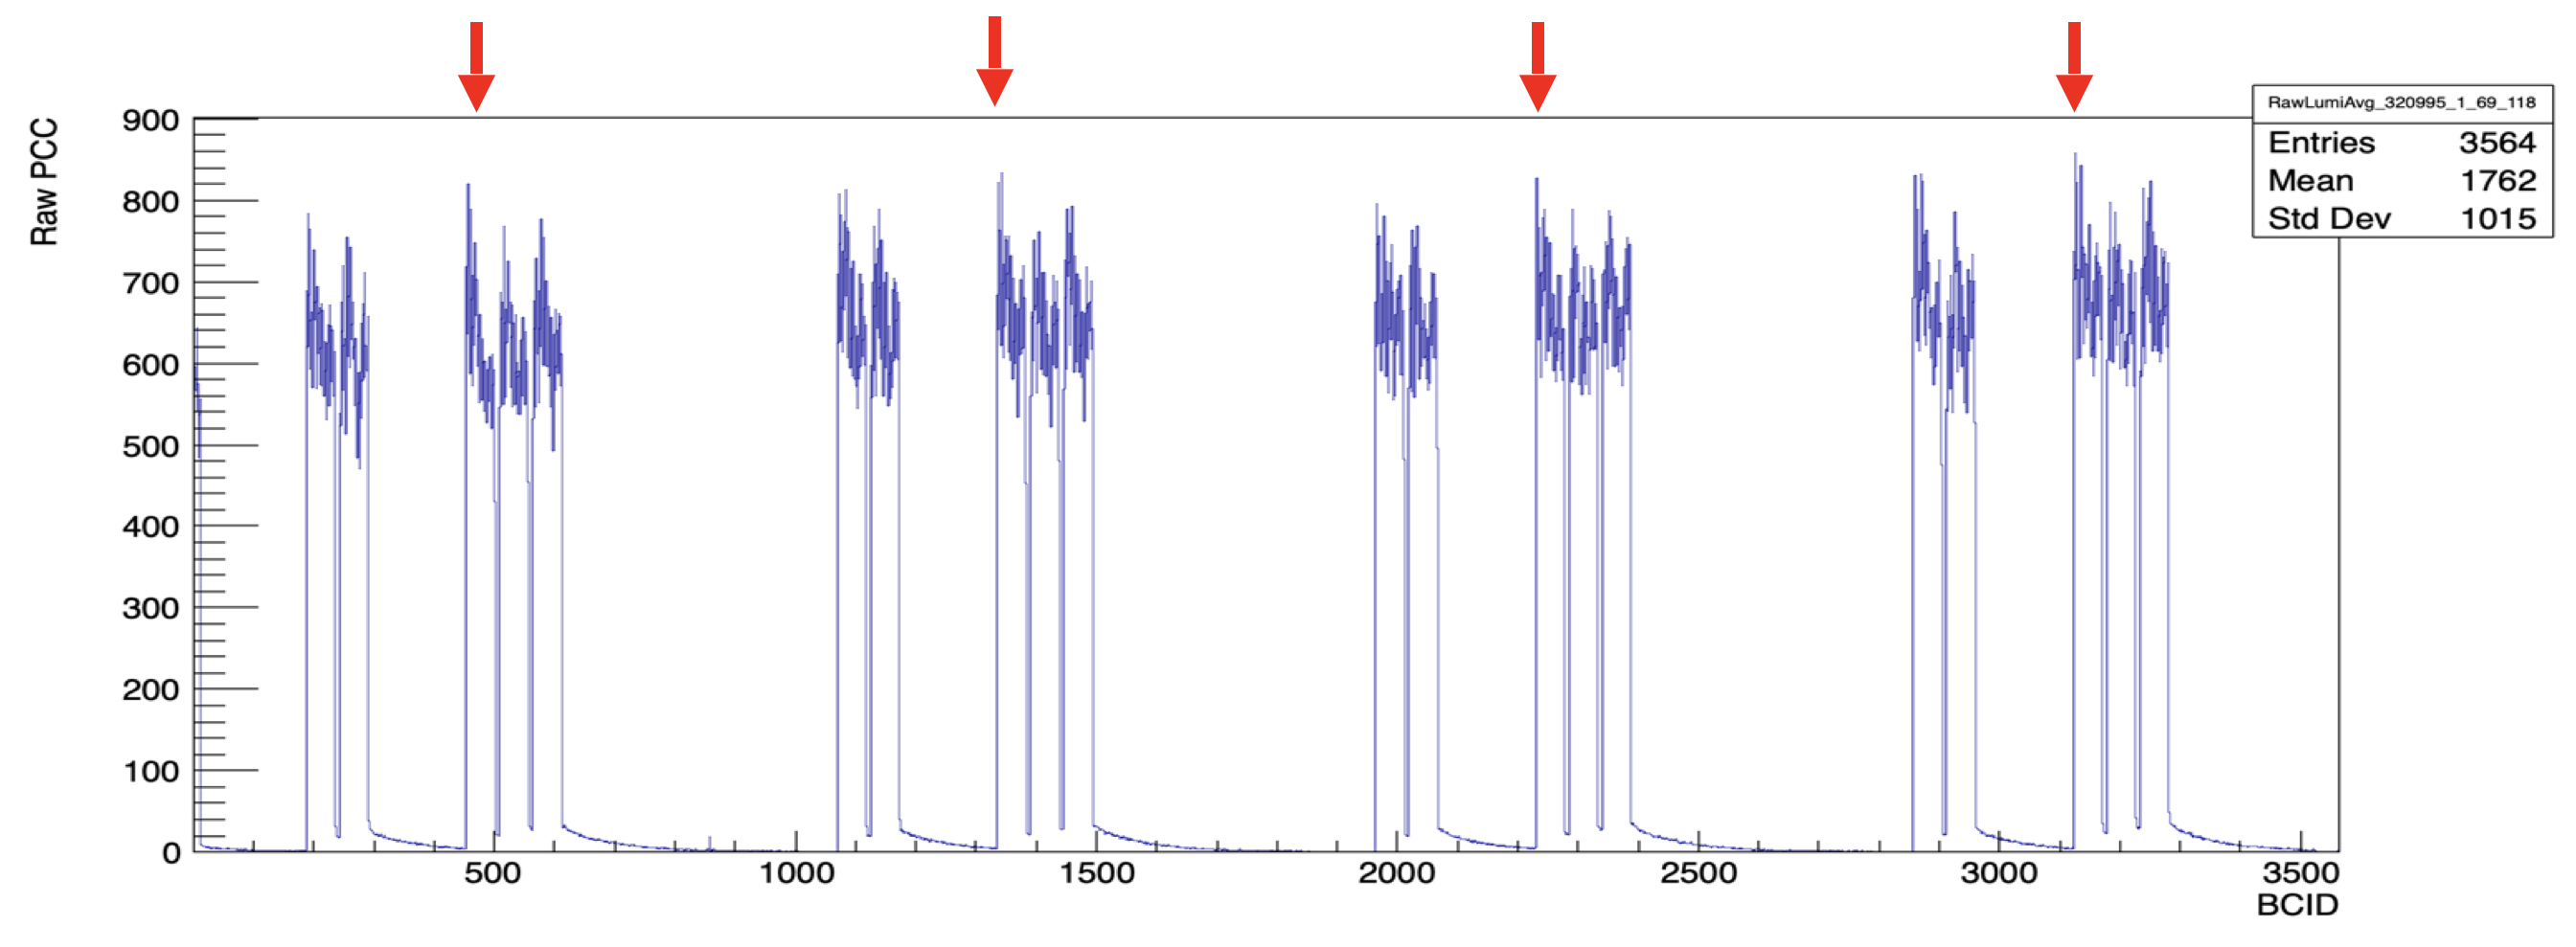
\includegraphics[width=1\textwidth]{ashish_thesis/3wagon_af.png}
%\caption[]{%                                                                                  
                                                                                                                                                                                                                                     
 % Afterglow fit model.
%}
%\label{fig:af_fit}
%\end{figure}

%\begin{figure}[!htp]
%\centering
%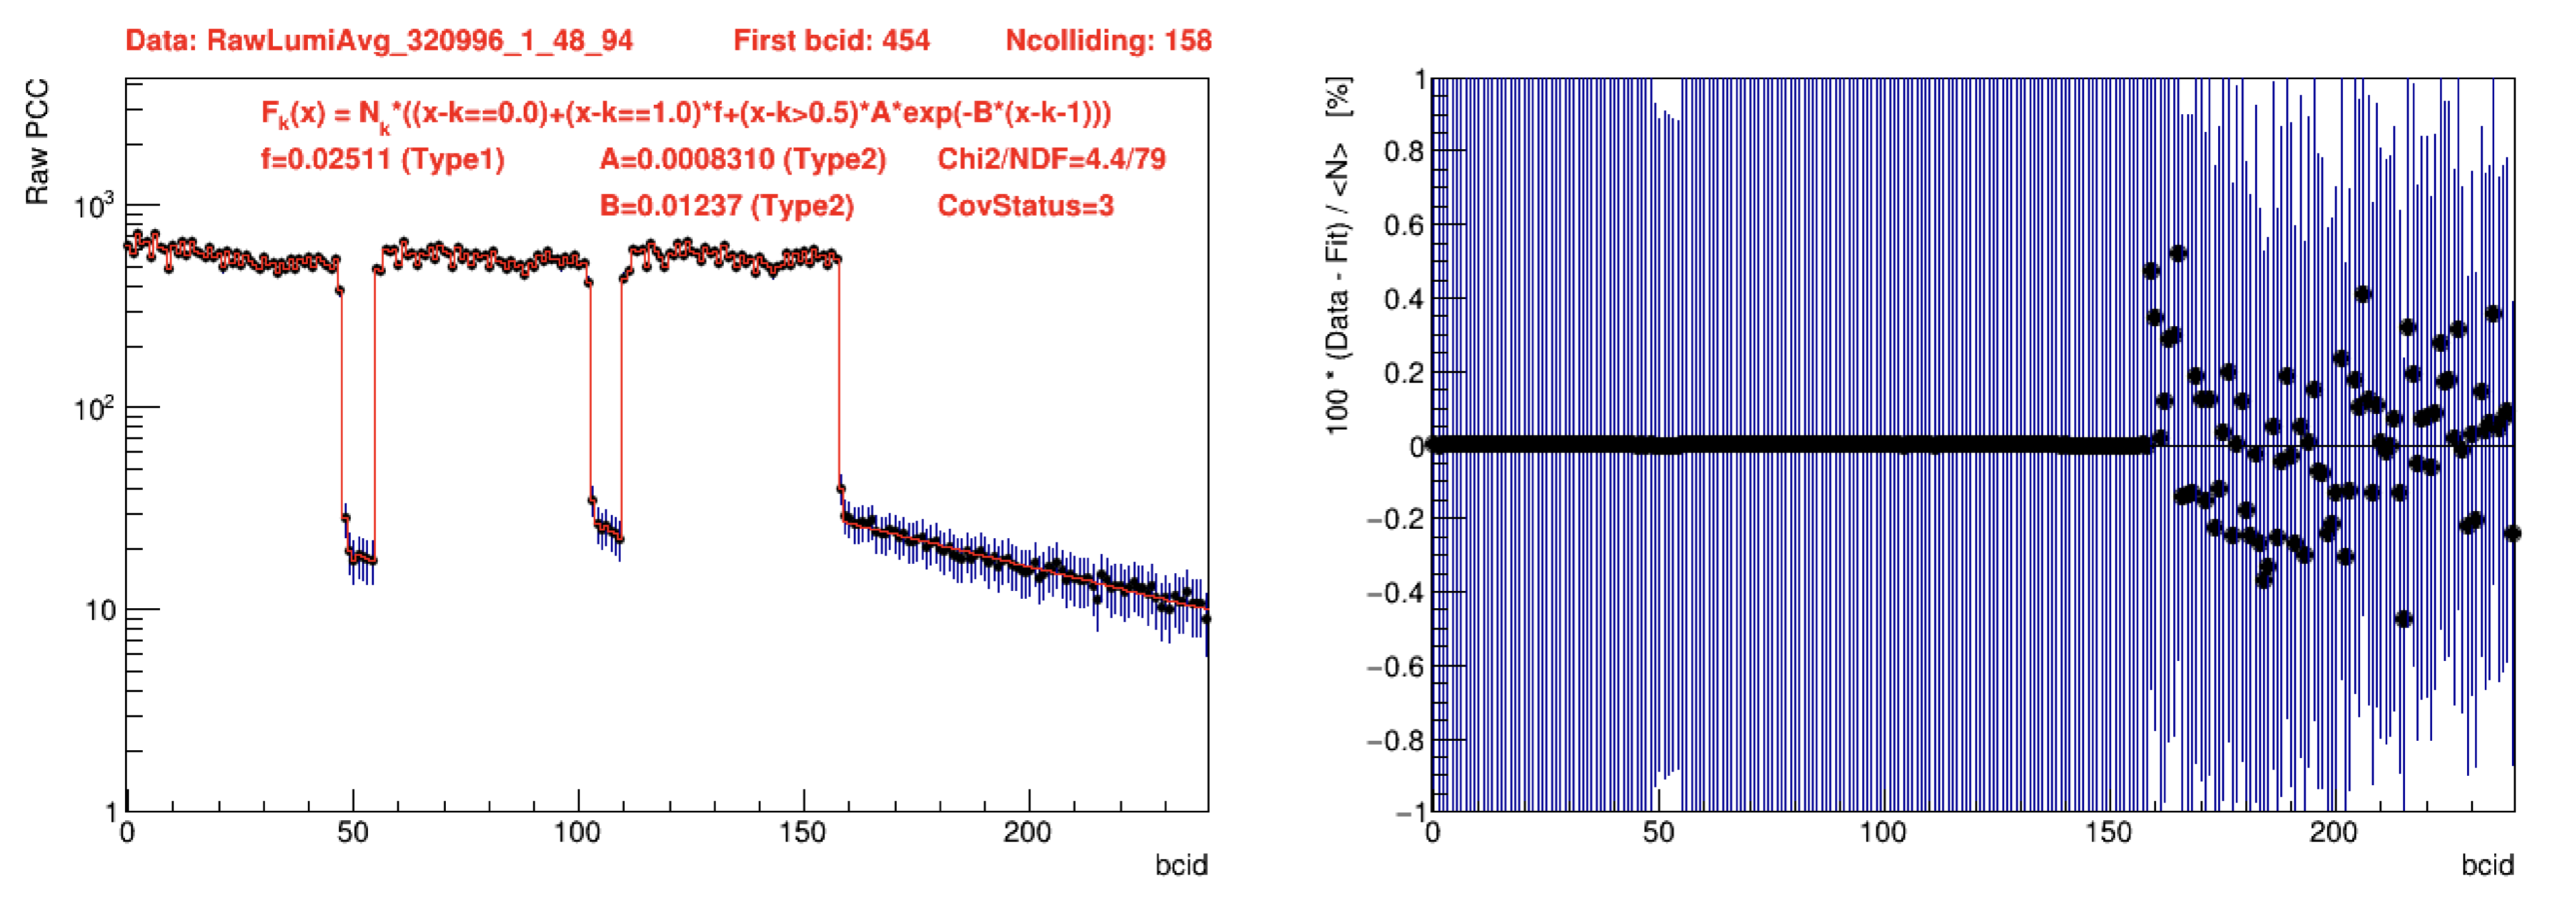
\includegraphics[width=1\textwidth]{ashish_thesis/3wagon_fit.png}
%\caption[Afterglow Fit]{%                                                                          
 % Afterglow fit model for 3 wagon train.
%}
%\label{fig:af_fit99}
%\end{figure}

\begin{figure}[H]
  \centering
    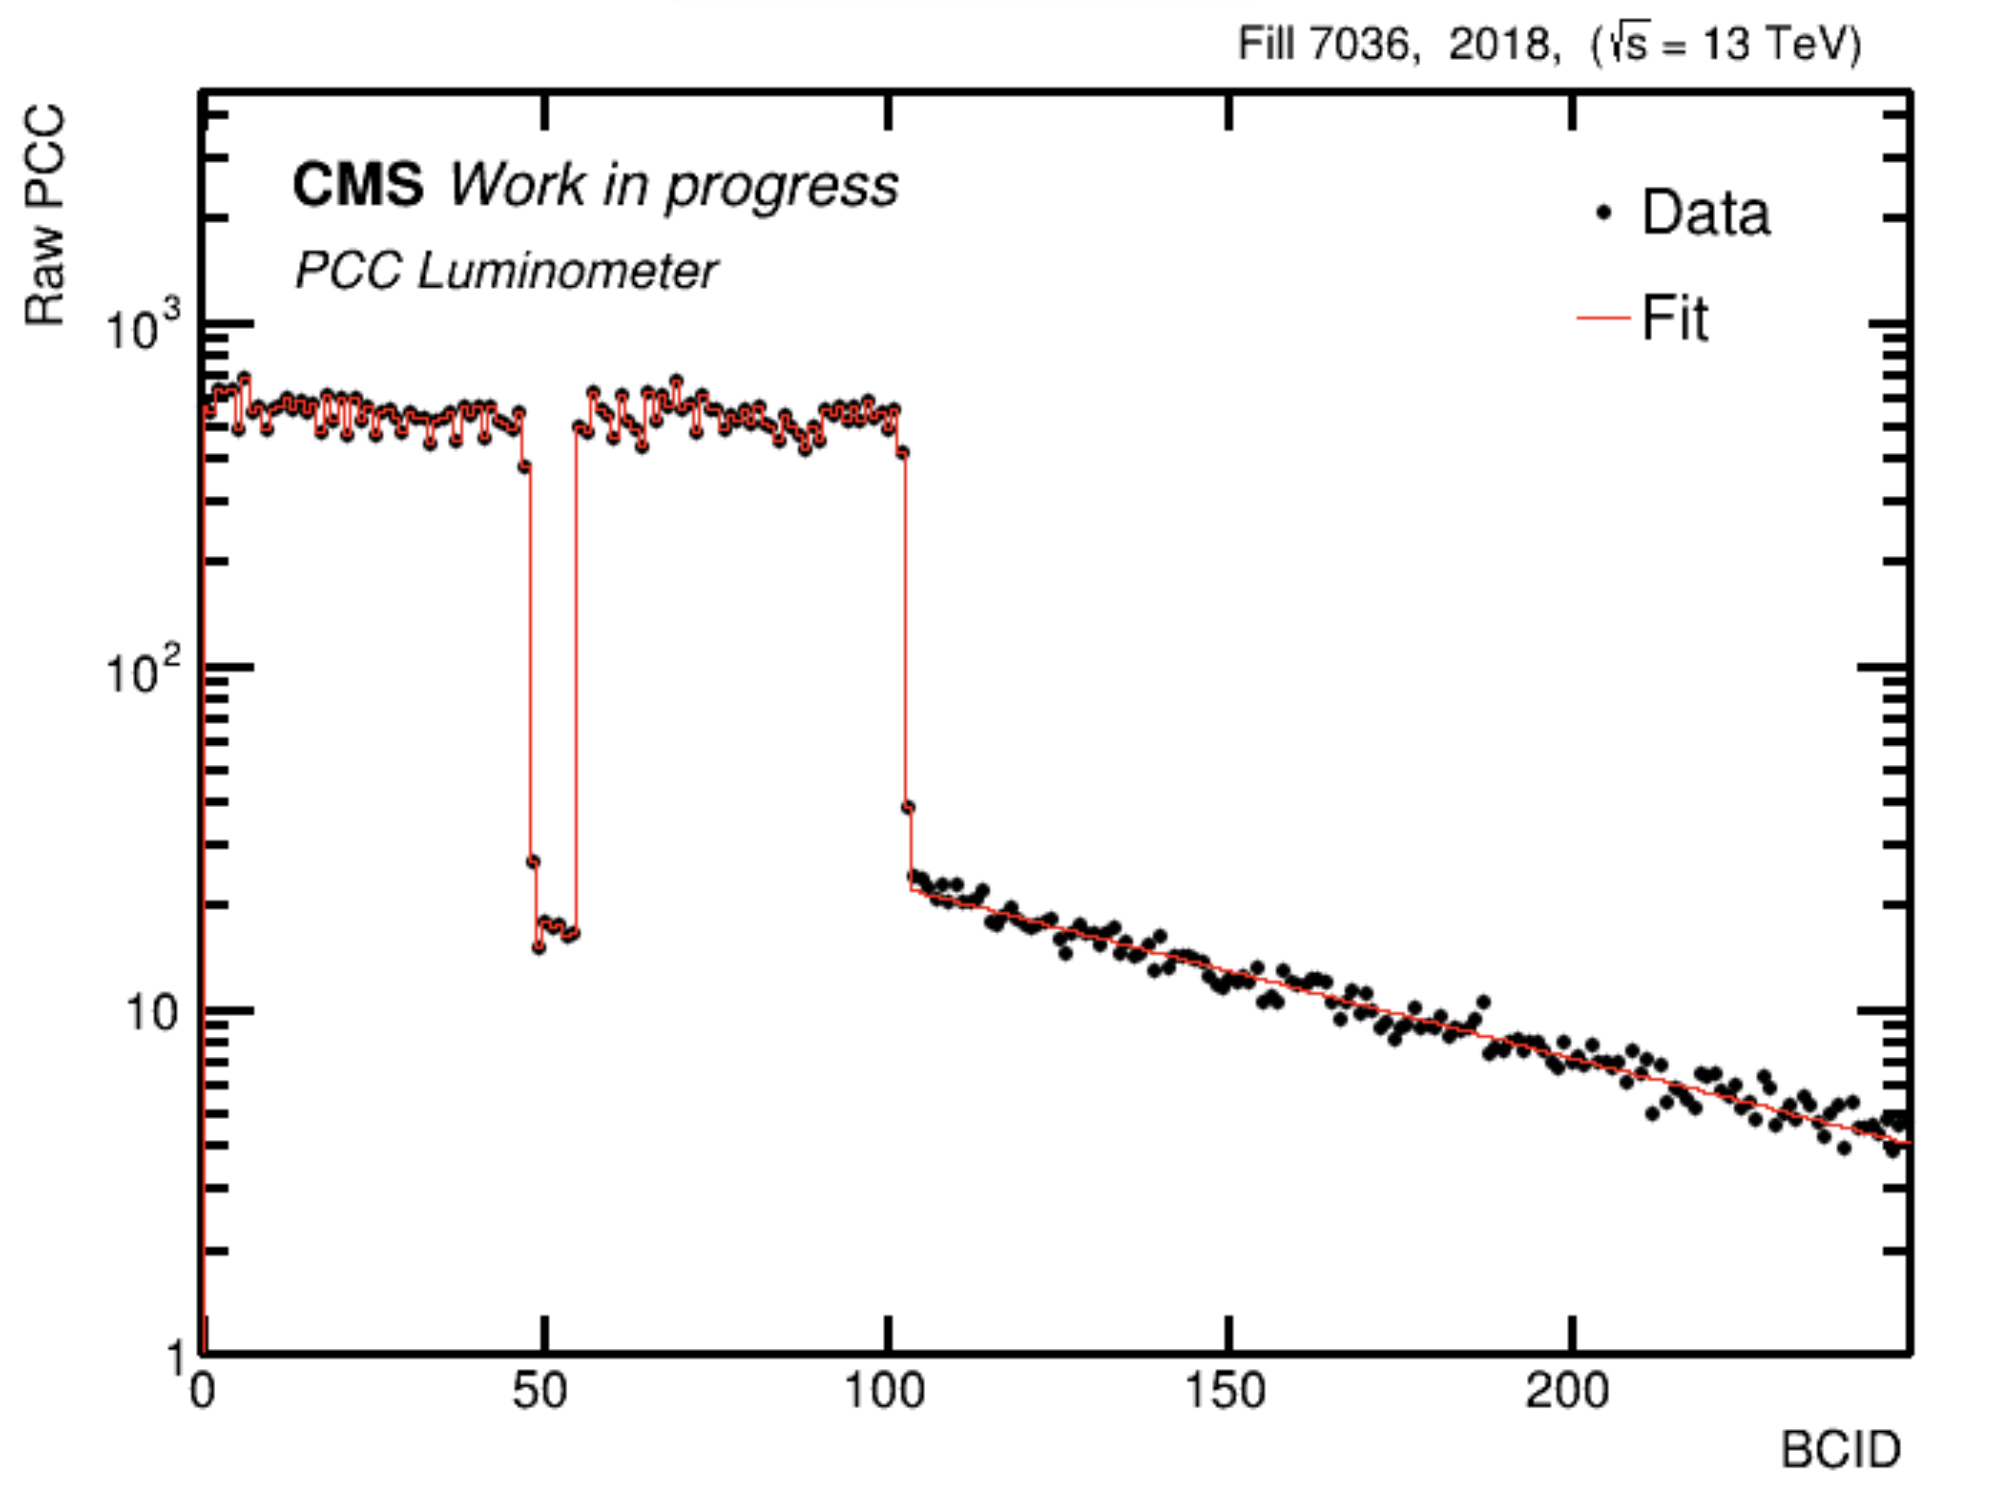
\includegraphics[width=0.75\textwidth]{ashish_thesis/2018_af_fit_1.png} 
  %\hfill % or \hspace{5mm} for a specific horizontal space                                                                                                  
  %\begin{subfigure}[b]{0.49\textwidth}
   % 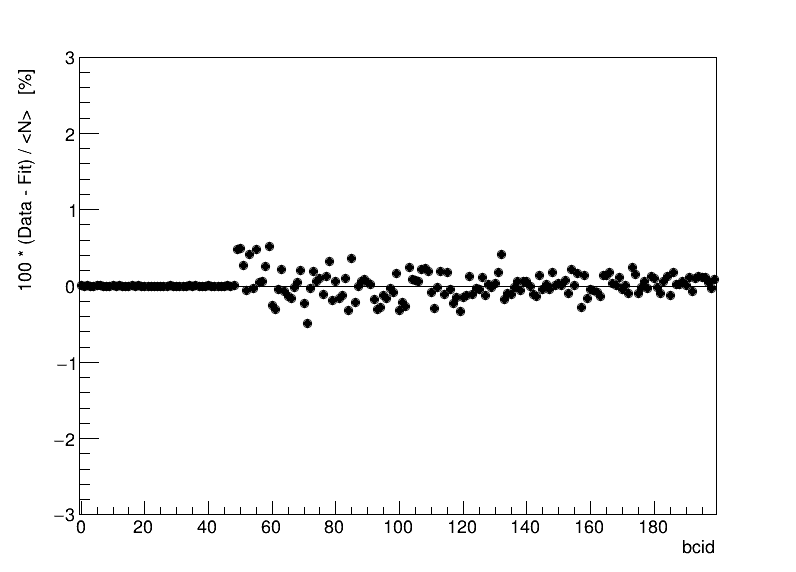
\includegraphics[width=\textwidth]{ashish_thesis/2018_af_fit_residuals.png}                                                                                     
  %\end{subfigure}
  \caption[Afterglow Effect Fit]{Fit to single train to estimate afterglow parameters.}
  \label{fig:af_fit99}
\end{figure}

%\begin{figure}[!htp]
%\centering
%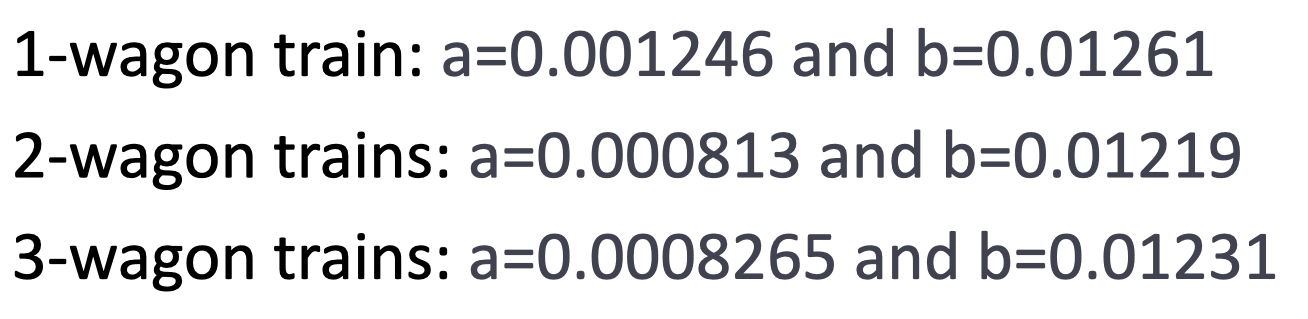
\includegraphics[width=1\textwidth]{ashish_thesis/type2_af_parameters.png}
%\caption[]{%                                                                                
 % Afterglow fit model.
%}
%\label{fig:af_fit}
%\end{figure}

%The values of type 2 afterglow parameter amplitude (a) and decay width (b) for different wagon trains are shown in Table \ref{fig:af_fit4000}.

\newpage
\begin{table}
  \centering
  \caption[Type 2 afterglow parameters estimation]{Type 2 afterglow parameters obtained from fit to raw pcc data}
  \begin{tabular}{ccc}
    \textbf{\# of wagon} & \textbf{B} & \textbf{C} \\
     \hline
   %1-wagon train  & 0.001246  & 0.01261 \\
   2-wagon train  & 0.000813 &  0.01219\\
   3-wagon train  & 0.0008265 &  0.01231\\
  \end{tabular}
  %\caption{Type 2 afterglow parameters obtained from fit to raw pcc data}
  \label{fig:af_fit4000}
\end{table}

The scale factor for one 50 lumi section block in run number 315690 is shown in Fig. \ref{fig:af_change_veto}. It provides an overview of the afterglow scale factor applied to the raw PCC. On the left, both the raw and corrected PCC for all bunch crossings are displayed, showing the variations between the initial data and the adjusted counts. The right side specifically highlights the afterglow scale factor for a single 50 lumi section block, representing the afterglow correction applied for final module veto.

\newpage
\begin{figure}[H]
\centering
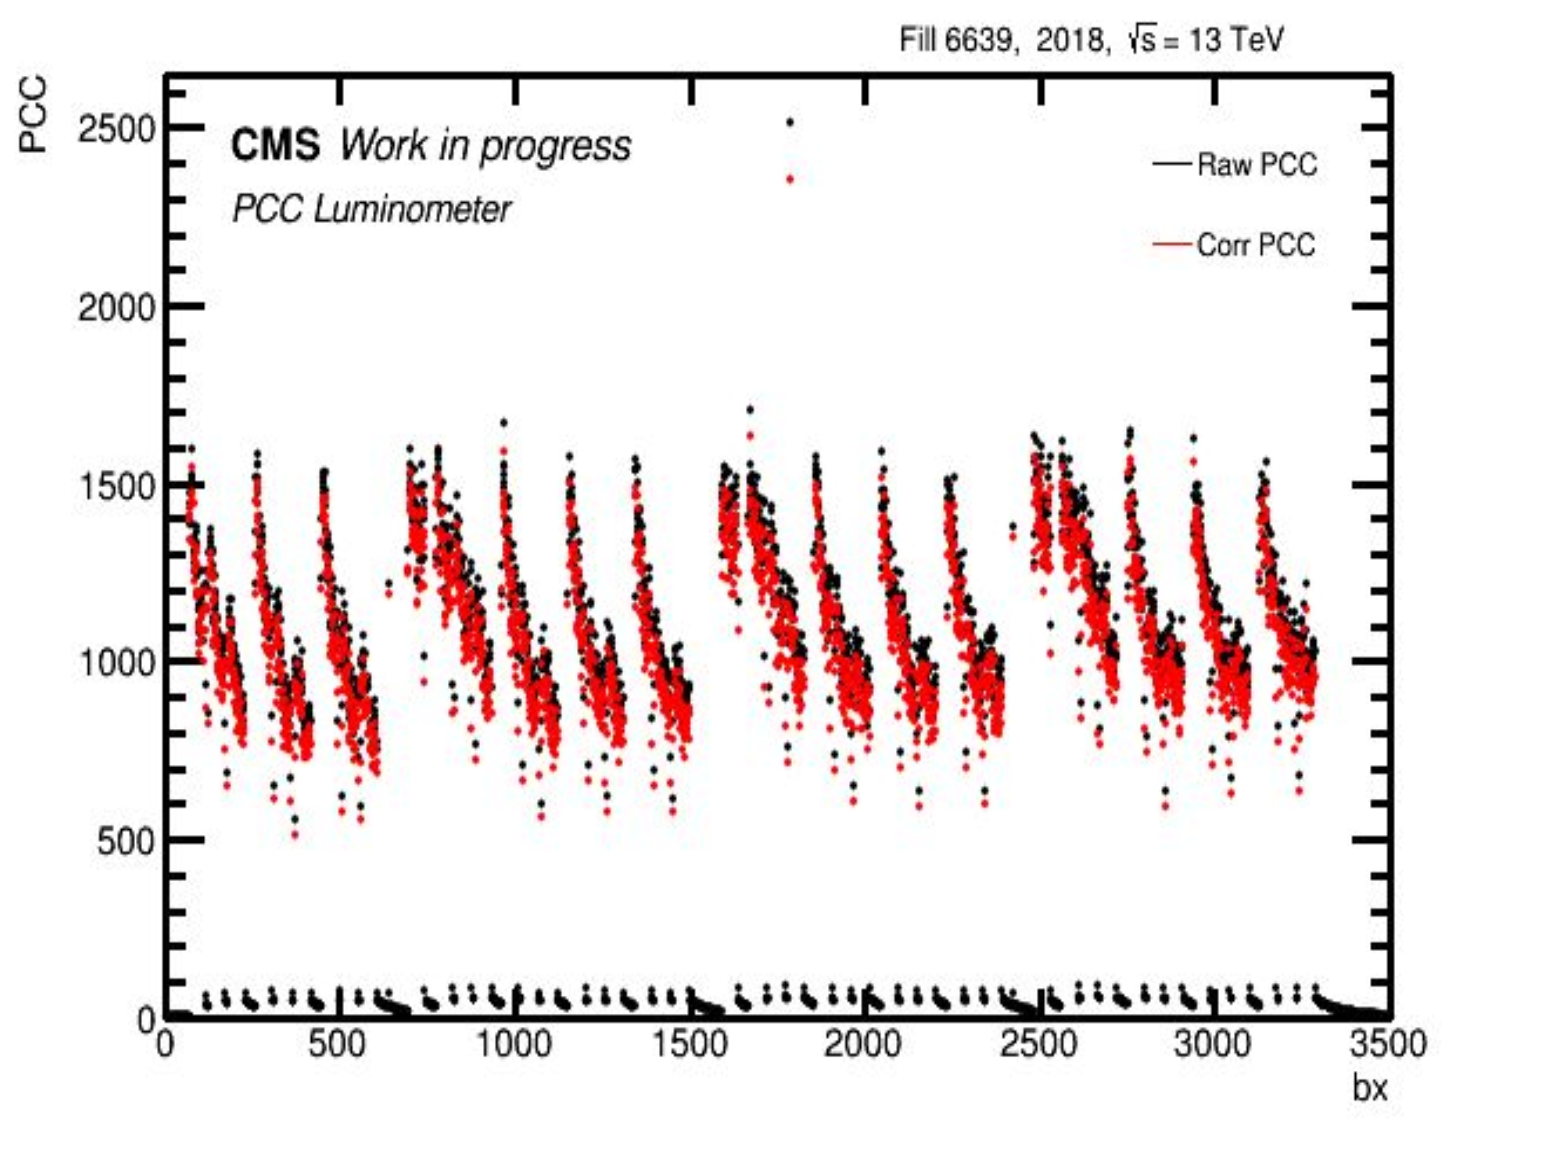
\includegraphics[width=0.8\textwidth]{ashish_thesis/afterglow_correction_factor_1lsblock_315690_2.png}
\caption[Run 315690 Afterglow Background]{%                                                                                                                                                                                                                                                                                                
 Raw and corrected PCC for all bunch crossings.
}
\label{fig:af_change_veto}
\end{figure}

\begin{figure}[H]
\centering
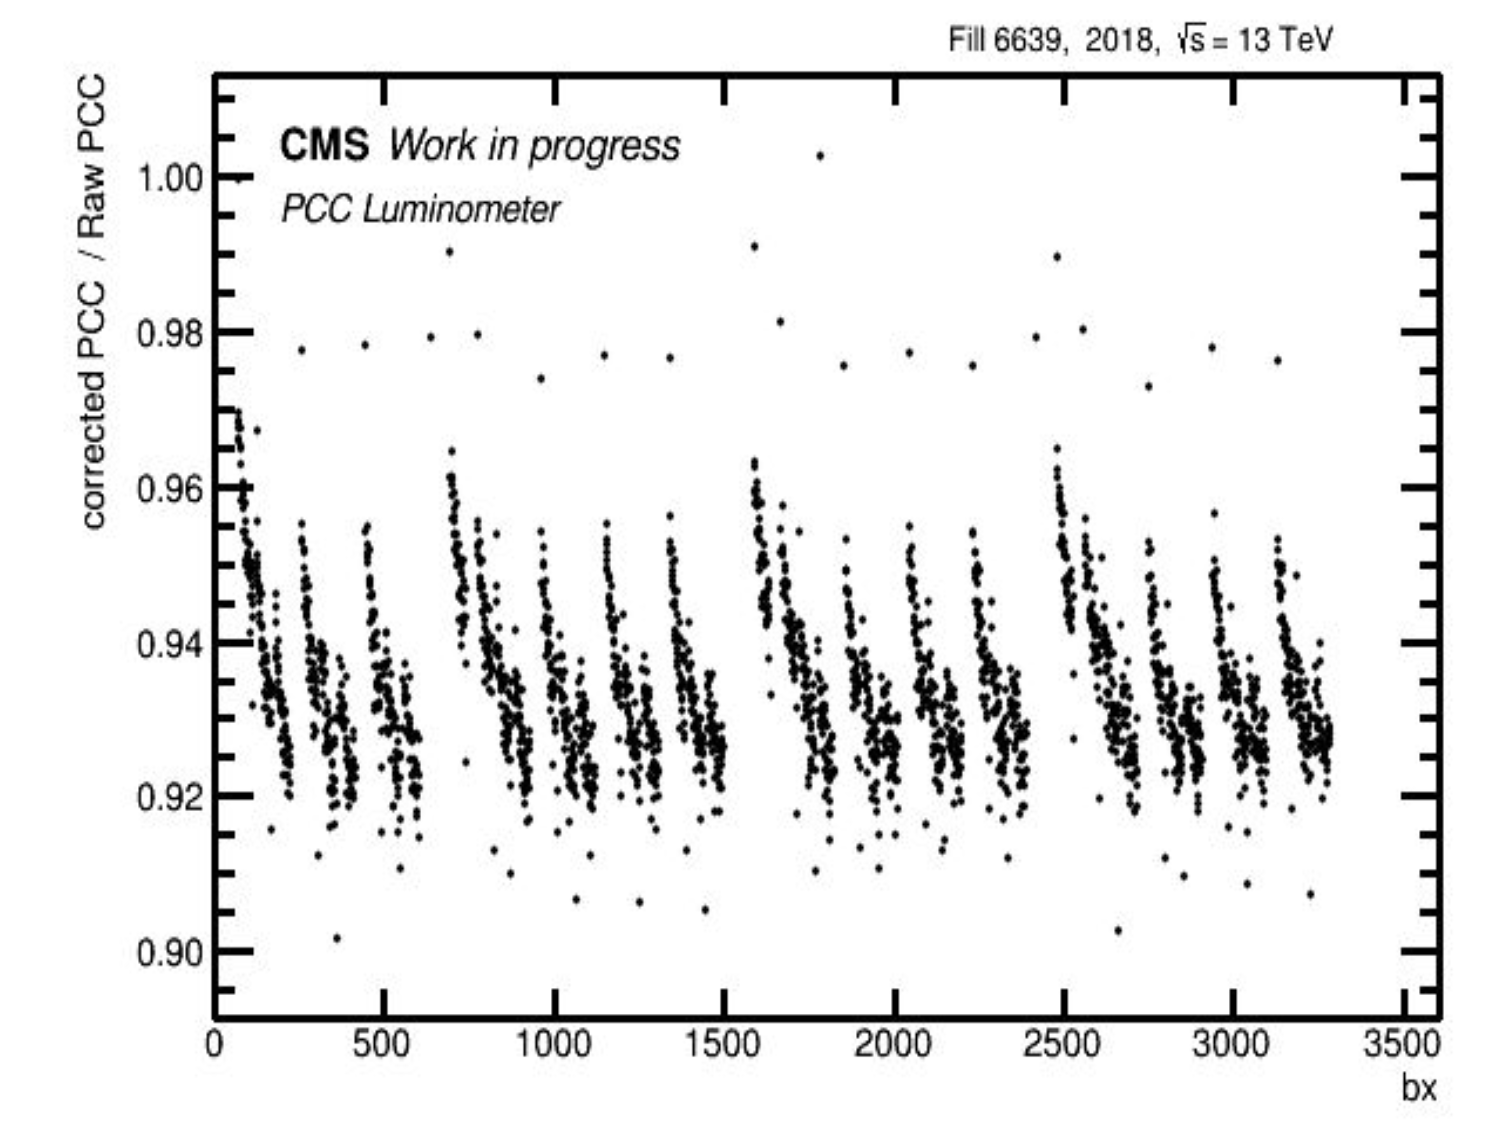
\includegraphics[width=0.8\textwidth]{ashish_thesis/afterglow_correction_factor_1lsblock_315690_3.png}
\caption[Run 315690 Afterglow Background]{%
  Afterglow scale factor for one 50 lumi section block in run 315690 for the final module veto.
}
\label{fig:af_change_veto}
\end{figure}


\section{PCC instantaneous and integrated luminosity}

Instantaneous luminosity is proportional to the rate of collisions at any given moment in time. It is a snapshot of the experiment's performance and is represented as \( L_{\text{inst}} \). The unit of instantaneous luminosity is often Hertz per micro barn $(Hz/ub)$. Integrated luminosity is the accumulation of instantaneous luminosity over a specific time period. Mathematically, it is defined as:
\[
\text{Integrated Luminosity} = \int (\text{Instantaneous Luminosity}) \, dt
\]
The unit of integrated luminosity is typically inverse femtobarns (\( \text{fb}^{-1} \)). Integrated luminosity can be understood as the sum of all instantaneous luminosities over the duration of the experiment, enhancing the statistical significance of the data collected. It serves as a measure of the total number of events recorded by the experiment, crucial for robust statistical analysis. When plotted as a function of lumi sections, PCC instantaneous and integrated luminosity offer distinct yet complementary insights into the experiment's performance. In plots that feature luminosity as a function of these lumi sections, the x-axis enumerates the lumi sections while the y-axis presents the luminosity values.  For instantaneous luminosity, discrete data points are plotted for each lumi section, providing immediate, lumi section specific measurements of the collision rate as shown in Fig. \ref{fig:PCC_inst_2018}. These points can fluctuate based on a variety of factors, such as beam conditions or adjustments to the accelerator. On the other hand, integrated luminosity is represented by a continuously ascending curve. %Each point on this curve accumulates the instantaneous luminosity values up to that specific lumi section. %The integrated luminosity for entire 2018 is calculated to be 60.47 fb^{-1}.

\begin{figure}[!htp]
\centering
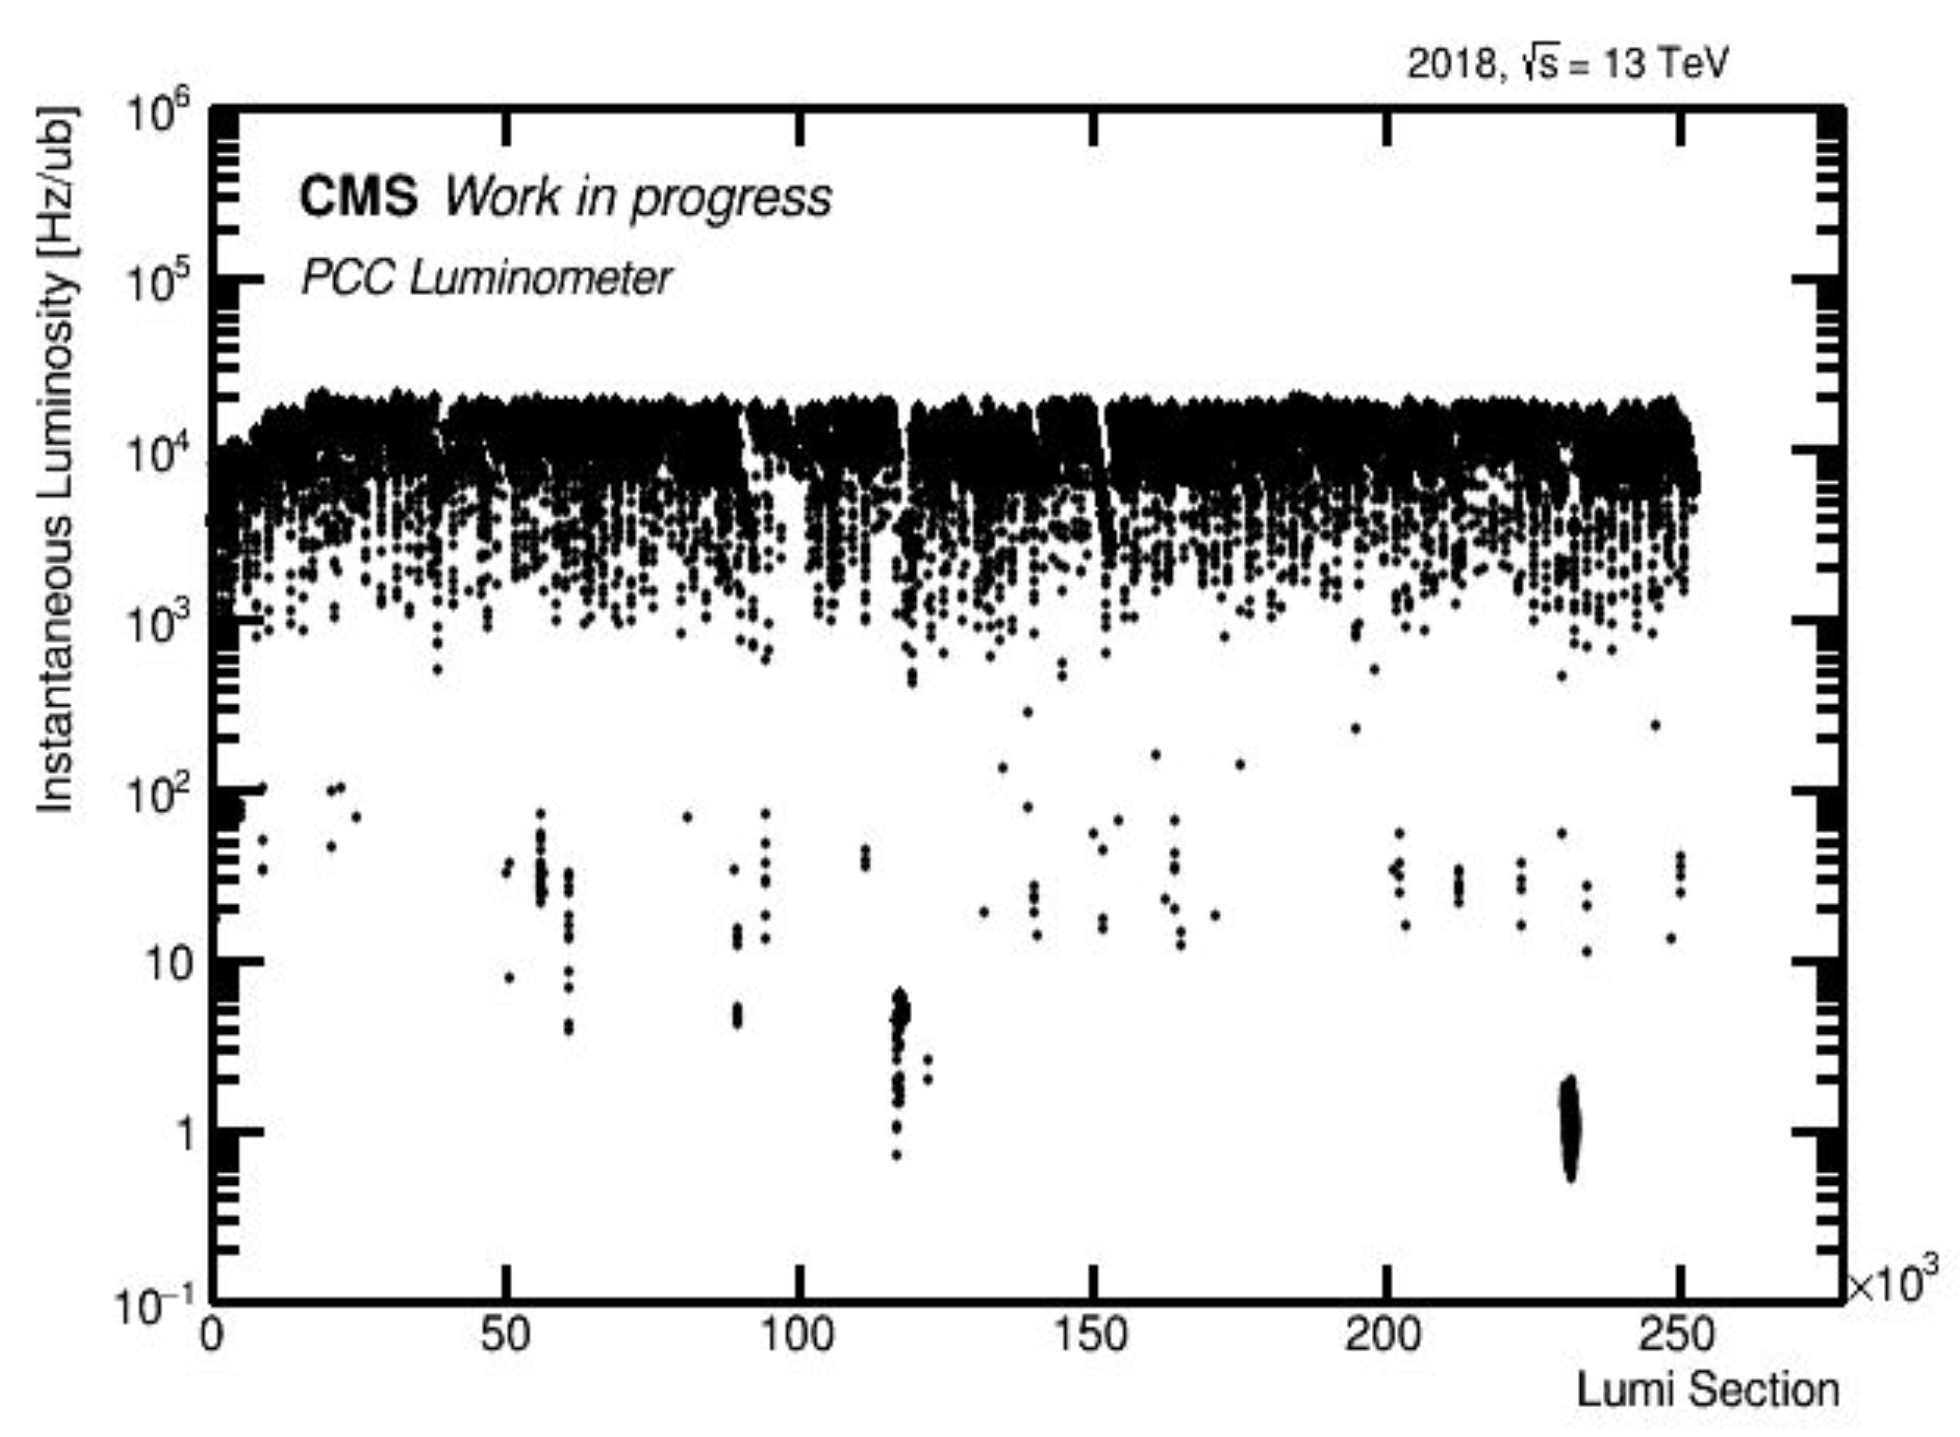
\includegraphics[width=1\textwidth]{ashish_thesis/PCClumivslumisection_2018_1.png}
\caption[2018 PCC Inst. Luminosity]{%                                                                                                                                                                   
 2018 PCC instantaneous luminosity as a function of lumi section.
}
\label{fig:PCC_inst_2018}
\end{figure}

\newpage
\section{Systematic uncertainties}

The luminosity measurement at CMS experiment is influenced by various systematic uncertainties. Systematic uncertainty originates from inherent biases in experimental design, instrumentation, or methodologies, consistently skewing results away from the true value. These include effects from orbit drifts, xy non-factorization, beam-beam interactions, stability issues, non-linearity of the detector response, afterglow from preceding collisions, and CMS deadtime. Each of these sources can impact the precision of the luminosity determination and requires careful consideration in the luminosity's data analysis.

\subsection{vdM calibration uncertainties}

\begin{itemize}

\item Orbit Drift: Orbit drift in particle accelerators refers to the slight deviation or shift in the trajectory of circulating particle beams from their intended path. This drift can be caused by a myriad of factors, including imperfections in the magnetic fields guiding the beams, external disturbances, and even minute ground movements or temperature fluctuations affecting the accelerator components. The precision with which beams are aligned in colliders like the LHC is crucial for maximizing the number of particle collisions, and hence the luminosity. When an orbit drift occurs, the overlap of the colliding beams may become suboptimal, leading to a reduced instantaneous luminosity. This reduction can influence the effectiveness of the experiments conducted, potentially introducing uncertainties in the luminosity measurement \cite{CERNOribLumi}.

\begin{comment}
    
Orbit drift refers to the changes in the orbit of the proton beams in the Large Hadron Collider (LHC) \cite{CERNOribLumi}. These beams are accelerated to near the speed of light, and any minor variations in the beam's path can lead to discrepancies in the observed data. This drift becomes particularly significant for precision measurements, such as those required for calculating the luminosity of collisions in the CMS experiment.

%Luminosity at CMS is a crucial quantity as it directly correlates to the number of potential collision events. The higher the luminosity, the more data available for scientists to analyze. Thus, the accurate measurement of luminosity is of paramount importance.

Orbit drift in the LHC can contribute to systematic uncertainties in the luminosity measurement in several ways:

Beam Position: Orbit drift can change the beam's position in the detector, which could affect the interaction rate and thus the measured luminosity. The systematic uncertainty in the luminosity due to orbit drift is associated with the precision of the correction techniques used to compensate for this drift.

Beam Size: Orbit drift can also alter the size and shape of the beam, which affects the beam's cross-sectional area. As the luminosity is inversely proportional to the cross-sectional area, changes in this parameter can lead to a systematic uncertainty in the luminosity.

Beam Angle: If the orbit drift changes the angle at which the beams collide, it could affect the effective overlap of the beams, again influencing the measured luminosity.

A high degree of precision in luminosity measurement requires a similarly precise knowledge of the beam's position and path. Orbit drift, therefore, poses a challenge. One common cause of orbit drift is the natural degradation of the magnetic field in the LHC's dipole magnets, which are responsible for steering the protons around the LHC ring.

Orbit drift correction in luminosity measurements at CMS is typically addressed by using a combination of real-time monitoring and post-experiment data corrections.

Real-time corrections: The LHC includes a Beam Position Monitor (BPM) system, which continuously tracks the position of the beams. If a drift is detected, the LHC's steering magnets can be adjusted to correct the orbit in real time. This adjustment is automated and relies on feedback loops.

Post-experiment corrections: After the data are collected, a detailed analysis of the recorded beam positions and luminosity is carried out. This analysis can detect and correct for any residual orbit drift that wasn't addressed in real time. This post-processing step involves detailed statistical analyses and machine learning algorithms to optimize the precision of the luminosity measurement.

\end{comment}

%Furthermore, simulations of the LHC beam dynamics are used to better understand the causes and effects of orbit drift, allowing the CMS experiment team to continuously improve their correction methods and achieve the best possible precision in their luminosity measurements.

%As the LHC continues to upgrade its hardware, including the upgrade to the High-Luminosity LHC, orbit drift will continue to be an important aspect to monitor and correct to ensure accurate and reliable results from the CMS and other experiments at CERN.

  %Refers to the gradual displacement of the beam orbit from its ideal trajectory due to various effects such as ground motion, magnetic field fluctuations, and thermal expansion. This can result in reduced beam intensity and beam quality

 %\cite{CERNOribLumi}.

\item  X-Y nonfactorization: The luminosity calibration often relies on methods that factorize the beam overlap integral into two separate integrals in the horizontal (X) and vertical (Y) directions. When this factorization is not valid or precise, the XY non-factorization comes into play. It essentially refers to the systematic uncertainty arising from the inability to perfectly separate or factorize the beam profiles in the horizontal and vertical dimensions. A variety of reasons can lead to XY non-factorization. One of the main causes is the complex shape and dynamics of the colliding beams. While in an ideal scenario, the beams might be perfectly Gaussian in shape and independent in X and Y dimensions, real-world effects such as beam-beam interactions, intrabeam scattering, or external perturbations can introduce correlations between the two dimensions. This means that the actual overlap of the beams cannot be simply represented as a product of their profiles in X and Y. The luminosity is a direct measure of how many collisions are happening per unit of time and area, and it depends on the overlap of the colliding beams. If the beams' profiles in the X and Y dimensions are not factorized correctly, it can lead to an inaccurate representation of their overlap, thus introducing a systematic uncertainty in the luminosity measurement \cite{CERNLUMPOG}.

%This is crucial because any error in luminosity calibration directly impacts the normalization of the cross-section measurements and, thus, the results and interpretations of the physics processes under study \cite{CERNLUMPOG}.

\begin{comment}

The nonfactorization of proton density distribution in the X-Y plane (i.e., the plane transverse to the direction of the beam in the accelerator) can introduce uncertainties in the measurement of luminosity \cite{CERNLUMPOG}.

In ideal conditions, the density distribution of the protons in each beam would be a perfect Gaussian distribution that is factorizable in the X and Y directions. That is, the distribution in the X direction would not depend on the position in the Y direction, and vice versa. However, in reality, this is often not the case due to various factors such as the design of the beam optics, beam-beam interactions.

The nonfactorizability of the proton density distribution means that the actual distribution of the protons in the beam deviates from the ideal Gaussian shape. The distribution can become asymmetric, or develop tails or other deformations. These deviations can lead to uncertainties in the luminosity measurement in several ways:

Interaction Rate: The luminosity is directly proportional to the overlap of the two beams at the collision point. If the density distribution is nonfactorizable, the overlap of the beams can be less (or more) than what would be predicted by assuming a factorizable distribution.

The nonfactorizability of the density distribution can also affect the effective size of the beam at the collision point.

%Beam Shape: The shape of the beam, which is determined by the density distribution of the protons, can also affect the luminosity. For example, a non-Gaussian beam shape can lead to a non-uniform spatial distribution of collision events in the detector, which can introduce uncertainties in the luminosity measurement.

%Refers to the failure of the x and y coordinates of a particle beam to factorize, meaning that the beam profile cannot be expressed as a product of independent x and y profiles. This can result in beam asymmetries and other effects
%\cite{CERNLUMPOG}.

\end{comment}

\item Beam-Beam Deflection: refers to the change in trajectory of the individual particles in the beam as they pass near each other in the interaction point, due to their electromagnetic interaction \cite{Herr:1982430}. In a perfect scenario, each beam of protons would stay focused and keep their trajectory constant throughout the process. However, when two beams cross each other, the electromagnetic fields of the protons in one beam can exert forces on the protons in the other beam, causing them to deviate from their initial trajectory \cite{babaev2023impact}.
  
%Refers to the mutual interaction of two colliding particle beams, resulting in the deflection of the individual beams due to the electromagnetic fields generated by the other beam. This effect can lead to beam losses and reduced luminosity \cite{CERNBeamBeam}
%\cite{Herr:1982430} \cite{babaev2023impact}.

\item Dynamic $\beta$: The beta function ($\beta$*) in the context of particle accelerators like the Large Hadron Collider (LHC) is a measure of the beam size at the collision point \cite{CERNVdMOMC}, and it plays a crucial role in determining the luminosity of the collisions. Lower values of $\beta$* lead to smaller beam sizes at the interaction point and thus higher luminosity, as the probability of proton-proton collisions is increased. However, $\beta$* is not necessarily constant during the operation of the LHC. It can vary due to factors such as changes in the accelerator's operating conditions, beam-beam interactions. %This variability, often referred to as "dynamic beta", can contribute to uncertainties in the luminosity measurement.
 When $\beta$* changes, it can alter the size of the proton beams at the interaction point. As the luminosity is inversely proportional to the square of the beam size, a small change in $\beta$* can lead to a significant change in luminosity. If these changes in $\beta$* are not accurately tracked and accounted for, they can introduce uncertainties in the luminosity measurement. The challenge is that $\beta$* is not directly observable, so its value and any changes in it have to be inferred from other measurements, such as the beam size and position, the orbit drift.
 %and so on. These measurements have their own uncertainties, which can further contribute to the uncertainty in β* and thus the luminosity.
  %Refers to the time-varying beta function of a particle beam, which describes the rate at which the beam diverges or converges as it propagates. This effect can be important for beam stability and the control of beam emittance
 % \cite{CERNVdMOMC}.

\item Beam Current Calibration:  Beam current calibration ensures that the \( N \) value (number of particles per bunch) used in the luminosity equation is accurate. If the calibration is off, the derived value of \( N \) from the instruments like beam current transformers will be inaccurate, leading to errors in the calculated luminosity \( L \). As the luminosity dependence on number of particles per bunch is \( N^2 \), even small errors in beam current calibration can significantly affect the accuracy of \( L \) \cite{CERNLumiDays}.

%Refers to the process of accurately measuring the current of a particle beam, which is essential for many beam diagnostics and control systems \cite{CERNLumiDays}.

\item Ghosts and Satellites: The ghost charge refers to the unintended or unexpected particles present in slots within the LHC beam that are nominally supposed to be empty. This term encapsulates the stray particles that aren't part of the primary, intended bunch structure of the beam. Ghost charges can originate from remnants of previous fills or injections into the LHC. When protons are injected and circulated within the accelerator, not all of them are perfectly grouped into the designated bunch structures. Some can linger outside the primary bunches, leading to these unintended ghost charges. The presence of ghost charges can significantly impact the luminosity measurement. Ghost charges can lead to additional, unexpected collisions when they interact with particles from the opposing beam. If these ghost-induced collisions are not accounted for, the luminosity can be overestimated. In the LHC, with its 400 MHz RF, there are 35640 RF bins, each about 2.5 ns long. Though only every tenth bin is typically filled with a particle bunch, stray particles are found in neighboring bins. These stray bunches within a \(\pm 12.5 \) ns range of a filled RF bin are termed \textit{"satellite bunches"}, distinct from main bunches and can influence precision luminosity measurement.
 \cite{Alici:1427728}.

  %Refers to unwanted signals in a detector or measurement system that can arise from various sources such as scattered radiation, electronic noise, or interference from other particles. These can lead to inaccurate measurements and reduced data quality \cite{Alici:1427728}.

\item Scan to Scan Variation: Refers to the variation in experimental results obtained from different scans or measurements, which can arise from various sources such as statistical fluctuations, instrument drift, or systematic errors.

\item Bunch to Bunch Variation: It means the $\sigma_{vis}$  varies from one bunch to another bunch.

%\begin{figure}[!htp]
%\centering
%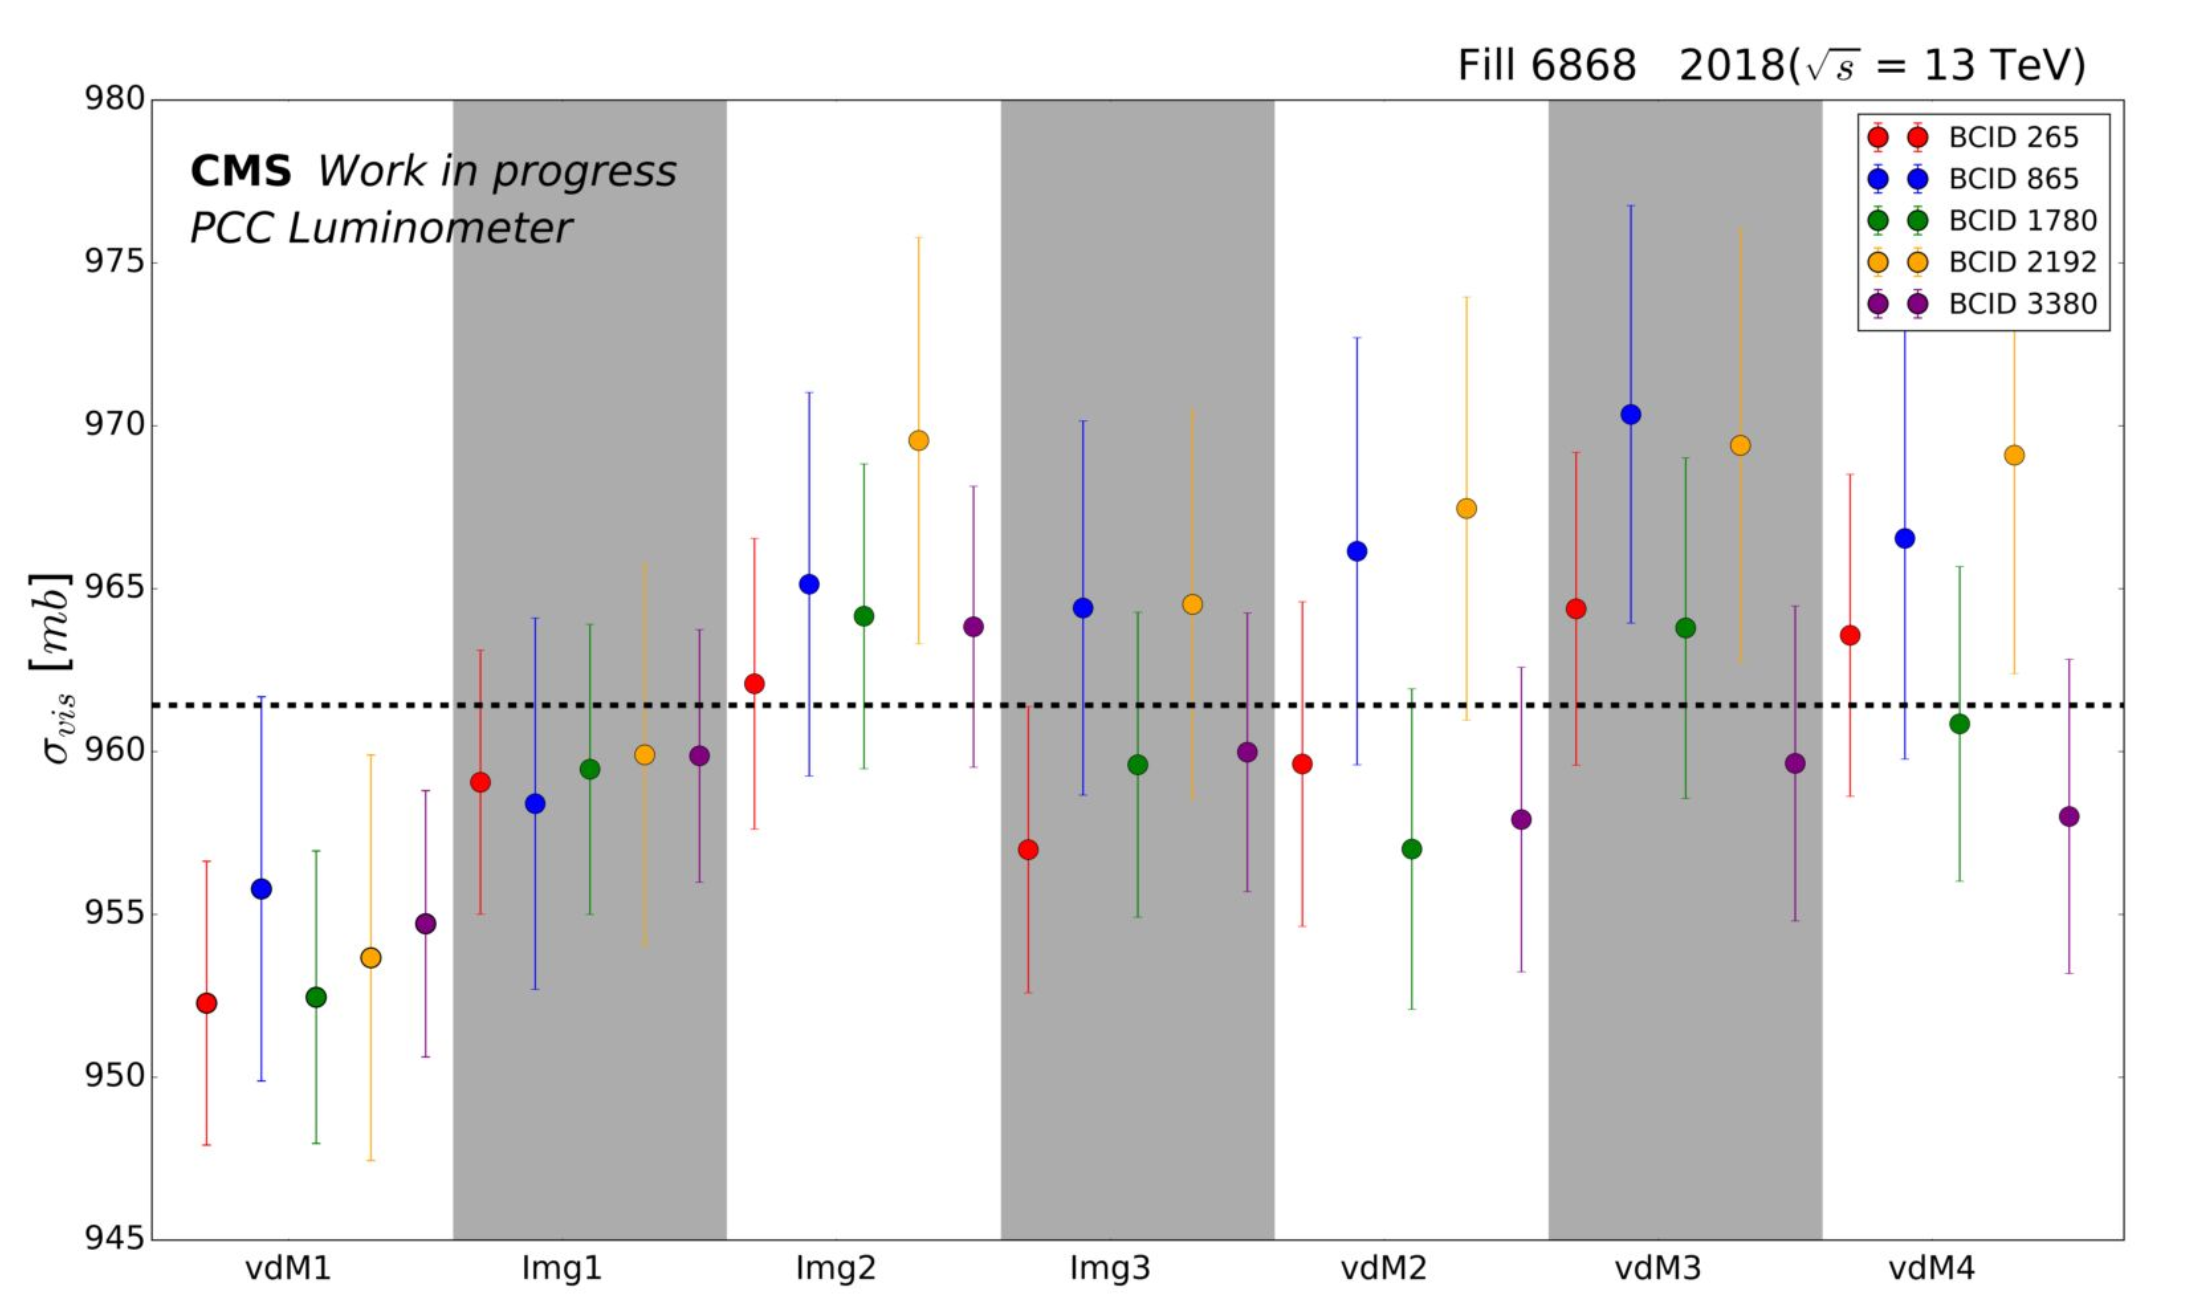
\includegraphics[width=0.7\textwidth]{ashish_thesis/sigma_vis_btob_var_1.png}
%\caption[$\sigma_{vis}$ Bunch Variation]{%                                                                                                                                                                   
 %Bunch to bunch variation of PCC visible cross section.  
%}
%\label{fig:sigmavis_btob_variation}
%\end{figure}

%\begin{tabular}{cccccc}
%\textbf{Scan} & \textbf{Mean} & \textbf{SEM} & \textbf{Standard Deviation} & \textbf{(Standard Deviation/Mean) $\times$ 100} \\
%\hline
%vdm1 & 953621.33 & 2148.68 & 1334.83 & 0.14\% \\
%Img1 & 959386.63 & 2050.61 & 559.37 & 0.058\% \\
%Img3 & 964376.43 & 2213.15 & 2502.04 & 0.26\% \\
%Img4 & 960386.85 & 2163.92 & 2936.50 & 0.31\% \\
%vdm2 & 960566.04 & 2425.60 & 4320.81 & 0.45\% \\
%vdm3 & 964566.94 & 2456.97 & 3928.54 & 0.41\% \\
%vdm4 & 962586.52 & 2419.86 & 3943.24 & 0.41\% \\
%\end{tabular}
%\caption[]{Scan to scan variation of PCC visible cross section. The “bunch spread” is determined from the standard deviation of the individual bunch-to-bunch uncertainty, averaged over all scans. The “bunch uncertainty” equal to the spread divided by the square root of the number of bunches.
%}

Table \ref{tab:sigmavis_btob_values} provides statistical data of the PCC visible cross-section for different scans. These scans represent different data-taking periods under slightly different experimental conditions. We observe that the 'Img1' scan has the smallest relative standard deviation, implying the least variability in the measured visible cross-section compared to its mean. On the other hand, the 'vdM2', 'vdM3', and 'vdM4' scans have higher relative standard deviations, indicating greater variability.

\begin{table}[h]
  \centering
  \caption[$\sigma_{vis}$ bunch variation uncertainty]{Bunch to bunch variation of PCC visible cross section. The “bunch spread” is determined as the standard deviation (STD) of the bunches divided by the mean. SEM is the standard error on the mean}
\begin{tabular}{cccccc}
\textbf{Scan} & \textbf{Mean} & \textbf{STD} & \textbf{(SEM/$\sigma_{vis}$) [\%]} \\
\hline
vdM1 & 953621.33 & 1334.83 & 0.14 \\
Img1 & 959386.63 & 559.37 & 0.058 \\
Img3 & 964376.43 & 2502.04 & 0.26 \\
Img4 & 960386.85 & 2936.50 & 0.31 \\
vdM2 & 960566.04 & 4320.81 & 0.45 \\
vdM3 & 964566.94 & 3928.54 & 0.41 \\
vdM4 & 962586.52 & 3943.24 & 0.41 \\
\end{tabular}
%\caption[Uncertainty due to bunch to bunch variation]{Bunch to bunch variation of PCC visible cross section. The “bunch spread” is determined as the standard deviation (STD) of the bunches divided by the mean.} %from the standard deviation of the individual bunch-to-bunch uncertainty, averaged over all scans. The “bunch uncertainty” equals the spread divided by the square root of the number of bunches.}
\label{tab:sigmavis_btob_values}
\end{table}

\item Cross-Detector Consistency: Refers to the agreement between measurements obtained from different detectors or measurement systems. This is important for verifying the accuracy and reliability of experimental results. A head-on lumi phase during vdm fill is used.

\item Background Subtraction: Refers to the process of removing unwanted signals from a measurement or detector system that arise from sources other than the physical phenomenon of interest, such as noise, cosmic rays, or other particles. Machine induced backgrounds are subtracted from raw PCC rate as described in section 4.3. %Corrected rate is given by the difference between the raw rate and the background rate. Uncertainty in the background propagate to uncertainty in the rate as follows,

\begin{comment}
 
\begin{figure}[!htp]
\centering
\includegraphics[width=1\textwidth]{ashish_thesis/SS_background.png}
\caption[]{%                                                                                                                                                                                                      
}
\label{fig:sigmavis_ss_backg}
\end{figure}

  
\begin{table}[ht]
  \begin{subtable}{0.5\linewidth}
    \centering
    \begin{tabular}{cc}
      \textbf{BCID} & \textbf{Mean} \\
      \hline
      265 & 0.02902 \\
      865 & 0.02572 \\
      1780 & 0.02862 \\
      2192 & 0.02729 \\
      3380 & 0.02882 \\
    \end{tabular}
    \caption{SS1_{avg}= 0.027894 \pm 0.01249}
  \end{subtable}%
  \begin{subtable}{0.5\linewidth}
    \centering
    \begin{tabular}{cc}
      \textbf{BCID} & \textbf{Mean} \\
      \hline
      265 & 0.02743 \\
      865 & 0.0281 \\
      1780 & 0.0286 \\
      2192 & 0.02323 \\
      3380 & 0.02896 \\
    \end{tabular}
    \caption{SS2_{avg}= 0.027264 \pm 0.00049}
  \end{subtable}
  \caption{SS bkg= 0.02757 +- 0.01987}
\end{table}

\end{comment}

%c_rate = r_rate - b_rate
%d(c_rate)square = d(r_rate)square + d(b_rate)square
%d(c_rate)/c = sqrt[d(r_rate)square + d(b_rate)square] /c
%d(c_rate)/c= d(b_rate)/c
%= 0.00049/4.6 = 0.000106 (0.01%)
%(delta sigma/sigma)square = (delta R/R) square

%\begin{equation}
%c_{rate} = r_{rate} - b_{rate}
%(dc_{rate})^2 = (dr_{rate})^2 + (db_{rate})^2
%\end{equation}

%\begin{equation}
%dc_{rate} = \sqrt{(dr_{\text{rate}})^2 + (db_{\text{rate}})^2}
%\end{equation}

%\begin{equation}
%$\frac{dc_{rate}}{c_{peak}}$ =$\frac{\sqrt{(dr_{\text{rate}})^2 + (db_{\text{rate}})^2}}{c_{peak}}$
%\end{equation}

%\begin{equation}
%$\frac{d(c_{\text{rate}})}{c_{peak}}$ = $\frac{d(b_{\text{rate}})}{c_{peak}}$
%\frac{0.00049}{4.6} = 0.000106 \text{ (0.01\%)}
%(\frac{\delta \sigma}{\sigma})^2 = (\frac{\delta R}{R})^2
%\end{equation}

\end{itemize}


\begin{comment}
  
\begin{equation}
c_{rate} = r_{rate} - b_{rate}
\end{equation}

\begin{equation}
(dc_{rate})^2 = (dr_{rate})^2 + (db_{rate})^2
\end{equation}

\begin{equation}
dc_{rate} = \sqrt{(dr_{\text{rate}})^2 + (db_{\text{rate}})^2}
\end{equation}

\begin{equation}

$\frac{dc_{rate}}{c_{peak}}$ =$\frac{\sqrt{(dr_{\text{rate}})^2 + (db_{\text{rate}})^2}}{c_{peak}}$

\end{equation}

\begin{equation}

$\frac{dc_{rate}}{c_{peak}}$ = $\frac{d(b_{rate})}{c_{peak}}$
  
%\frac{0.00049}{4.6} = 0.000106 \text{ (0.01\%)}                                                                                                                                                                                                                              
%(\frac{\delta \sigma}{\sigma})^2 = (\frac{\delta R}{R})^2                                                                                                                                                                                                     
\end{equation}

%\end{comment}                                                                                                                                                        

\begin{equation}
c_{\text{rate}} = r_{\text{rate}} - b_{\text{rate}}
\end{equation}

\begin{equation}
(dc_{\text{rate}})^2 = (dr_{\text{rate}})^2 + (db_{\text{rate}})^2
\end{equation}

\begin{equation}
dc_{\text{rate}} = \sqrt{(dr_{\text{rate}})^2 + (db_{\text{rate}})^2}
\end{equation}

\begin{equation}
\frac{dc_{\text{rate}}}{c_{\text{peak}}} = \frac{\sqrt{(dr_{\text{rate}})^2 + (db_{\text{rate}})^2}}{c_{\text{peak}}}
\end{equation}

\begin{equation}
\frac{dc_{\text{rate}}}{c_{\text{peak}}} = \frac{db_{\text{rate}}}{c_{\text{peak}}}
\end{equation}

\end{comment}

\subsection{Integration uncertainties}

\begin{itemize}

\item Stability: Systematic uncertainties can be introduced due to time-dependent changes in detector performance and environmental conditions. These changes can be influenced by various factors, including detector aging, radiation damage, and fluctuations in noise. A comparison of PCC luminosity with HFOC luminosity as a function of time is shown in Fig. \ref{fig:stabprof_7098} depicting slight instabilities in PCC luminosity over time.
%Detector Aging and Radiation Damage Detectors used in high-energy physics experiments are subject to aging and radiation damage due to the high-intensity radiation environment they operate in.
Detector aging can result in time-dependent changes in the detector's performance. For example, as the detector ages or sustains radiation damage, its efficiency may decrease, leading to a reduction in the number of detected events for a given luminosity. %This effect is typically modeled and accounted for in the data analysis, but any inaccuracies in the modeling can introduce a systematic uncertainty.
Fluctuation in the  noise level in the detector can also fluctuate over time due to changes in the experimental conditions. Noise can lead to spurious signals that can be misinterpreted as genuine events, leading to an overestimate of the luminosity. Conversely, high noise levels can also mask genuine events, leading to an overestimate of the luminosity. %Noise can be suppressed using data analysis techniques, but this is not always perfect, and residual noise can introduce a systematic uncertainty.
The standard deviation of ratio of luminosity from best and second best luminometer is used as stability systematic uncertainty as shown in Fig. \ref{fig:stabprof1}. The standard deviation provides a measure of the spread or dispersion of the measurements. If the measurements are stable, the spread will be small, and the standard deviation will be low. Conversely, if there are time-dependent changes in the detector performance or environmental conditions, the measurements will vary more, and the standard deviation will be higher.

  %It arises from time-dependent changes in detector performance or environmental conditions, Detector aging, radiation damage, fluctuation in noise. The standard deviation of ratio of luminosity from first and second best luminometeris used as stability systematic uncertainty.

  %The CMS pixel detector is a complex instrument with many components, including silicon sensors and readout electronics, that must operate consistently and with high precision over long periods. Any variations in the performance of the detector can affect the efficiency of the pixel cluster counting method and lead to uncertainties in the luminosity measurement.

  %One example of how the stability of the detector can affect the luminosity measurement is through changes in the detector's noise level. The noise level refers to the level of electronic noise present in the detector, which can interfere with the detection of pixel clusters produced by proton-proton collisions. If the noise level increases, the efficiency of the pixel cluster counting method may decrease, leading to an underestimation of the luminosity. Conversely, if the noise level decreases, the efficiency of the method may increase, leading to an overestimation of the luminosity.

  %Another example is changes in the efficiency of the pixel detector. The efficiency of the detector refers to the fraction of proton-proton collisions that produce pixel clusters that can be detected and counted by the method. Any changes in the efficiency of the detector, for example due to changes in the gain or response of the silicon sensors, can lead to uncertainties in the luminosity measurement.

  %To mitigate these uncertainties, the CMS collaboration performs regular calibrations and monitoring of the detector performance, as well as cross-checks with other luminosity measurement techniques

  %Systematic uncertainties due to stability in the detector itself for the pixel cluster counting method are typically estimated by studying the performance of the method over time and comparing it to simulations or other measurements. Uncertainties due to changes in the noise level and detector efficiency are typically estimated separately and combined to obtain the total systematic uncertainty


\begin{figure}[!htp]
\centering
\includegraphics[width=0.8\textwidth]{ashish_thesis/PCC_HFOCvsls_ProfileX_all_1.png}
\caption[Luminosity Ratio Profile]{Profile of the PCC/HFOC luminosity as a function of lumi section.}
\label{fig:stabprof_7098}
\end{figure}

%\begin{figure}[h]
 % \centering
  %\begin{subfigure}[b]{0.49\textwidth}
   % \includegraphics[width=\textwidth]{ashish_thesis/PCC_HFOCvsls_ProfileX_all.png}
    %\caption{Image 1}                                                                                                                                                                  
  %\end{subfigure}
  %\hfill % or \hspace{5mm} for a specific horizontal space                                                                                                                              
  %\begin{subfigure}[b]{0.49\textwidth}
   % \includegraphics[width=\textwidth]{ashish_thesis/PCCvsHFOC_ProjectionY_all.png}
    %\caption{Image 2}                                                                                                                                                                  
  %\end{subfigure}
  %\caption[Stability of PCC luminosity compared to HFOC]{Left: Profile of the PCC/HFOC luminosity as a function of lumi section. Right: Histogram filled with the ratio of PCC/HFOC luminosity per lumi section.}
%\label{fig:stabprof}
%\end{figure}

\begin{figure}[!htp]
\centering
\includegraphics[width=0.8\textwidth]{ashish_thesis/ProjY_ProfileX_h_ratio_all_1.png}
\caption[Projection Of Luminosity Ratio Profile]{%                                                                                                                                                                            
Distribution of the ratio of PCC/HFOC luminosity evaluated per 50 lumi section blocks. 
}
\label{fig:stabprof1}
\end{figure}
  
%\begin{figure}[!htp]
%\centering
%\includegraphics[width=1\textwidth]{ashish_thesis/stability_sys.png}
%\caption[]{%                                                                                                                                                                                                                 
 % Stability systematic uncertainty.
%}
%\label{fig:af_fit}
%\end{figure}

\newpage
\item Linearity: The response of a detector might not always be the same at different luminosity levels. In other words, a detector might respond differently when there are more particles passing through it per unit of time (higher luminosity) compared to when there are fewer particles (lower luminosity). This is particularly relevant at the high luminosities achieved. Linearity of PCC luminosity with HFOC luminosity is shown in Fig. \ref{fig:stabprof2}. 
%Pileup Conditions Affect the Linearity of Luminosity Measurement
Pileup events are common at high luminosities and can affect the linearity of the luminosity measurement. If the detector or the counting system is unable to accurately count the number of pileup events, the count rate might not increase linearly with the actual luminosity, leading to a non-linear response. %This could introduce a systematic bias in the luminosity measurement, especially at high luminosities.
%High Pileup Can Cause Over- or Underestimation of Luminosity
%At high pileup conditions, the counting system may fail to distinguish between individual particle events and hence underestimate the actual number of particles, leading to an underestimation of the luminosity. Conversely, pileup can also potentially lead to overestimation of the luminosity if multiple particles are mistakenly counted as a single, more energetic particle.
%The Product of Slope and Luminosity Range is a Measure of Linearity Systematic Uncertainty
%In a perfect scenario, the  rate should increase linearly with the luminosity, and the slope of this relationship should be constant. However, due to non-linearities in the detector response, the slope can vary depending on the luminosity level as shown in Fig. \ref{fig:lin_unc}. This variability in the slope can be used to quantify the linearity systematic uncertainty.

A linear fit is done to study change in detector response at different luminosity levels. By multiplying the slope by the luminosity range (the difference between the highest and lowest luminosity levels), we obtain a measure of how much the  rate is expected to vary due to non-linearity over that luminosity range. This product can be used as an estimate of the linearity systematic uncertainty in the luminosity measurement.

  %the luminosity obtained from the PCC method is compared to that obtained from the HFOC method for a given set of collisions. Any deviations between the two measurements are used to estimate the linearity uncertainty in the PCC method.

  %The linearity uncertainty is typically quantified as a systematic uncertainty in the luminosity measurement, expressed as a percentage of the measured luminosity. This uncertainty can be estimated by fitting the PCC and HFOC measurements to a linear function and calculating the deviation of the PCC measurement from the linear fit.

%\begin{figure}[!htp]
%\centering
%\includegraphics[width=1\textwidth]{ashish_thesis/linearity_sys.png}
%\caption[]{%                                                                                                                                                                                               %                 \
                                                                                                                                                                                                                        
 % Linearity systematic uncertainty.
%}
%\label{fig:af_fit}
%\end{figure}



%\begin{figure}[!htp]                                                                                                                                                                   
%\centering                                                                                                                                                                             
%\includegraphics[width=0.6\textwidth]{ashish_thesis/PCC_HFOCvsHFOC_ProfileX_all.png}                                                                                                     
%\caption[]{%                                                                                                                                                                           
 %  Ratio of PCC/HFOC luminosity plotted as a function of HFOC luminosity to determine change in detector response over different luminosity levels. Slope of the linear fit is 2.34306e-07.                                                                                                                                                          
%}
%\label{fig:lin_unc}
%\end{figure}

%%\begin{table}[h]
 % \centering
  % \caption[Fit PCC luminosity]{Parameter values from fit}
   % \begin{tabular}{ccccc}
    %     Parameter Name & Value & Error \\
     %   \hline
      %   Slope &  7.21854e-07 & 7.61113e-09  \\
       %  Intercept & 9.86768e-01 & 1.17605e-05  \\
    %\end{tabular}
    %\caption{Parameter values from fit}
    %\label{tab:lin_fit}
%\end{table}

 
%\begin{figure}[h]
%  \centering
 % \begin{subfigure}[b]{0.49\textwidth}
  %  \includegraphics[width=\textwidth]{ashish_thesis/PCCvsHFOC_ProfileX_Fill6961_1.png}
    %\caption{Image 1}                                                                                                                                                                 
  %\end{subfigure}
  %\hfill % or \hspace{5mm} for a specific horizontal space                                                                                                                             
 % \begin{subfigure}[b]{0.49\textwidth}
  %  \includegraphics[width=\textwidth]{ashish_thesis/PCC_HFOCvsHFOC_ProfileX_Fill6961_1.png}
    %\caption{Image 2}                                                                                                                                                                 
  %\end{subfigure}
  %\caption[2018 PCC linearity]{Left: Linearity of PCC compared to HFOC for fill 6961. Right: Ratio of PCC/HFOC luminosity plotted as a function of HFOC luminosity to determine change in detector response over different luminosity levels. Slope of the linear fit is 7.2e^{-7} $in units of$ (Hz/ub)^{-1}.}
%\label{fig:stabprof2}
%\end{figure}


\begin{figure}[h]
  \centering
  \includegraphics[width=1\textwidth]{ashish_thesis/PCCvsHFOC_ProfileX_Fill6961_2.png}
  \caption[2018 PCC linearity]{Left: Linearity of PCC compared to HFOC for fill 6961. Right: Ratio of PCC/HFOC luminosity plotted as a function of HFOC luminosity to determ\
ine change in detector response over different luminosity levels. Slope of the linear fit is 7.2e^{-7} $in units of$ (Hz/ub)^{-1}.}
  \label{fig:stabprof2}
\end{figure}

\newpage
\item Afterglow: Systematic uncertainty due to afterglow background are determined by calculating the mean of the type 1 and type 2 afterglow residuals that are defined as the ratio of the luminosity of the first empty bunch immediately following a colliding bunch to the luminosity of the colliding bunch and ratio of the luminosity of the second and following empty bunches after a colliding bunch to the luminosity of the colliding bunch respectively.

  %Type 1 afterglow refers to the persistence of charge in the pixels of the detector after a collision event. This charge can be produced by various sources, such as ionization due to the passage of charged particles, or leakage currents in the readout electronics. If this charge is not properly accounted for, it can be mistakenly counted as pixel clusters produced by subsequent collision events, leading to an overestimation of the luminosity.

  %Type 2 afterglow refers to the persistence of noise in the detector after a collision event. This noise can be produced by various sources, such as thermal or radiation-induced effects, and can also interfere with subsequent collisions. If this noise is not properly accounted for, it can lead to a reduction in the efficiency of the pixel cluster counting method and an underestimation of the luminosity.

%\begin{figure}[!htp]
%\centering
%\includegraphics[width=1\textwidth]{ashish_thesis/type1_res.png}
%\caption[]{%                                                                                                                                                                                                      
 %  Type 1 residual.                                                                                                                                                                                                              
%}
%\label{fig:type1}
%\end{figure}

%\begin{figure}[h]
 % \centering
  %\begin{subfigure}[b]{0.49\textwidth}
   % \includegraphics[width=\textwidth]{ashish_thesis/type1res_gr0p5.png}
    %\caption{Image 1}                                                                                                                                                                  
  %\end{subfigure}
  %\hfill % or \hspace{5mm} for a specific horizontal space                                                                                                                              
  %\begin{subfigure}[b]{0.49\textwidth}
   % \includegraphics[width=\textwidth]{ashish_thesis/type2res_gr0.5_rangefixed.png}
    %\caption{Image 2}                                                                                                                                                                 
  %\end{subfigure}
  %\caption[PCC Afterglow Residuals]{Left: PCC afterglow correction type 1 residual as a function of instantaneous luminosity. The residual fraction is given by the ratio of the luminosity of the first empty bunch immediately following a colliding bunch to the luminosity of the colliding bunch. Right: Type 2 residual as a function of instantaneous luminosity. These are given by the ratio of the luminosity of the second and following empty bunches after a colliding bunch to the luminosity of the colliding bunch. Random trigger PCC dataset for all periods are used to make these plots \cite{Sehrawat2023}.}
%\label{fig:stabprof}
%\end{figure}

\begin{figure}[h]
  \centering
  \includegraphics[width=1\textwidth]{ashish_thesis/type1res_gr0p5_1.png}
  \caption[PCC Afterglow Residuals]{Left: PCC afterglow correction type 1 residual as a function of instantaneous luminosity. The residual fraction is given by the ratio of\
 the luminosity of the first empty bunch immediately following a colliding bunch to the luminosity of the colliding bunch. Right: Type 2 residual as a function of instantane\
ous luminosity. These are given by the ratio of the luminosity of the second and following empty bunches after a colliding bunch to the luminosity of the colliding bunch. Ra\
ndom trigger PCC dataset for all periods are used to make these plots \cite{Sehrawat2023}.}
  \label{fig:stabprof_4012}
\end{figure}



%\begin{figure}[!htp]
%\centering
%\includegraphics[width=1\textwidth]{ashish_thesis/type1res_gr0p5.png}
%\caption[]{%                                                                                                                                                                                              
 %  Type 1 residual.                                                                                                                                                                                       

%}
%\label{fig:type1}
%\end{figure}



%\begin{figure}[!htp]
%\centering
%\includegraphics[width=1\textwidth]{ashish_thesis


%\begin{figure}[!htp]
%\centering
%\includegraphics[width=1\textwidth]{ashish_thesis/type2res_gr0.5_rangefixed.png}
%\caption[]{%                                                                                                                                                                                              
 % Type 2 residuals.  Mean value is 0.00267652.
 %}
%\label{fig:type2}
%\end{figure}


%\begin{figure}[!htp]
%\centering
%\includegraphics[width=1\textwidth]{ashish_thesis/type1res_frac.png}
%\caption[]{%                                                                                                                                                                                                             
 %  Type 1 residual fraction.                                                                                                                                                                                                    
%}
%\label{fig:type2}
%\end{figure}

\end{itemize}

%\begin{figure}[!htp]
%\centering
%\includegraphics[width=0.6\textwidth]{ashish_thesis/type1frac_gr0p5.png}
%\caption[]{%                                                                                                                                                                                              
 %  Type 1 afterglow fraction as a function of single-bunch instantaneous luminosity. Random trigger PCC dataset for all periods are used to make this plot.                                               }
%\label{fig:type2}
%\end{figure}

\end{itemize}


%\begin{figure}[!htp]
%\centering
%\includegraphics[width=1\textwidth]{ashish_thesis/h_ProfileX_PCC_HFOCvsHFOC_all.png}
%\caption[]{%                                                                                                                                                         
                                                                                                                                                                     
 %  Type 1 residual fraction.                                                                                                                                         

%}
%\label{fig:type2}
%\end{figure}

%\begin{figure}[h]
 % \centering
  %\begin{subfigure}[b]{0.49\textwidth}
   % \includegraphics[width=\textwidth]{ashish_thesis/PCC_HFOCvsls_ProfileX_all.png}
    %\caption{Image 1}
  %\end{subfigure}
  %\hfill % or \hspace{5mm} for a specific horizontal space
  %\begin{subfigure}[b]{0.49\textwidth}
   % \includegraphics[width=\textwidth]{ashish_thesis/PCCvsHFOC_ProjectionY_all.png}
    %\caption{Image 2}
  %\end{subfigure}
  %\caption{Left: }
%\label{fig:stabprof}
%\end{figure}
  



%\begin{figure}[!htp]
%\centering
%\includegraphics[width=0.6\textwidth]{ashish_thesis/ProjY_ProfileX_h_ratio_all.png}
%\caption[]{%                                                                                                                                                                         
 %  Type 1 residual fraction.
%}
%\label{fig:type2}
%\end{figure}





%\begin{figure}[!htp]
%\centering
%\includegraphics[width=1\textwidth]{ashish_thesis/PCC_HFOCvsHFOC_ProfileX_all.png}
%\caption[]{%                                                                                                                                                          
 %  Type 1 residual fraction.

%}
%\label{fig:type2}
%\end{figure}





%\begin{figure}[!htp]
%\centering
%\includegraphics[width=1\textwidth]{ashish_thesis/PCC_HFOCvsHFOC_ProfileX_residuals_all.png}
%\caption[]{%                                                                                                                                                         
 %  Type 1 residual fraction.

%}
%\label{fig:type2}
%\end{figure}




%\begin{figure}[!htp]
%\centering
%\includegraphics[width=1\textwidth]{ashish_thesis/PCC_HFOCvsls_all.png}
%\caption[]{%                                                                                                                                                         
 %  Type 1 residual fraction.

%}
%\label{fig:type2}
%\end{figure}




%\begin{figure}[!htp]
%\centering
%\includegraphics[width=1\textwidth]{ashish_thesis/PCC_HFOCvsls_ProfileX_all.png}
%\caption[]{%                                                                                                                                                         
 %  Type 1 residual fraction.

%}
%\label{fig:type2}
%\end{figure}


%\begin{figure}[!htp]
%\centering
%\includegraphics[width=1\textwidth]{ashish_thesis/PCCvsHFOC_all.png}
%\caption[]{%                                                                                                                                                         

 %  Type 1 residual fraction.

%}
%\label{fig:type2}
%\end{figure}



%\begin{figure}[h]
%  \centering
 % \begin{subfigure}[b]{0.49\textwidth}
  %  \includegraphics[width=\textwidth]{ashish_thesis/PCCvsHFOC_ProfileX_all.png}
    %\caption{Image 1}                                                                                                                                                                
  %\end{subfigure}
  %\hfill % or \hspace{5mm} for a specific horizontal space                                                                                                                            
  %\begin{subfigure}[b]{0.49\textwidth}
   % \includegraphics[width=\textwidth]{ashish_thesis/PCCvsHFOC_ProfileX_residuals_all.png}
    %\caption{Image 2}                                                                                                                                                                
  %\end{subfigure}
  %\caption{Left: }
%\label{fig:stabprof}
%\end{figure}


%\begin{figure}[!htp]
%\centering
%\includegraphics[width=1\textwidth]{ashish_thesis/PCCvsHFOC_ProfileX_all.png}
%\caption[]{%                                                                                                                                                         

 %  Type 1 residual fraction.

%}
%\label{fig:type2}
%\end{figure}




%\begin{figure}[!htp]
%\centering
%\includegraphics[width=1\textwidth]{ashish_thesis/PCCvsHFOC_ProfileX_residuals_all.png}
%\caption[]{%                                                                                                                                                         
 %  Type 1 residual fraction.

%}
%\label{fig:type2}
%\end{figure}

%\begin{figure}[!htp]
%\centering
%\includegraphics[width=1\textwidth]{ashish_thesis/PCCvsHFOC_ProjectionY_all.png}
%\caption[]{%                                                                                                                                                         

 %  Type 1 residual fraction.

%}
%\label{fig:type2}
%\end{figure}



%\begin{figure}[!htp]
%\centering
%\includegraphics[width=1\textwidth]{ashish_thesis/ProjY_ProfileX_h_ratio_all.png}
%\caption[]{%                                                                                                                                                         
 %  Type 1 residual fraction.
%}
%\label{fig:type2}
%\end{figure}

The systematic uncertainty during 2018 luminosity measurement for final veto is shown in Table \ref{tab:systematic-uncertainty}.  

\begin{comment}
X-Y Nonfactorization: The uncertainty associated with the assumption of independent proton distributions in the X and Y dimensions decreases from 2\% under the PAS veto to 0.4\% under the final veto.

Bunch to Bunch Variation: The uncertainty related to variability between different bunches of protons reduces from 0.3\% under the PAS veto to 0.1\% under the final veto.


Background Subtraction: The uncertainty from the process of estimating and subtracting background noise reduces from 0.1\% under the PAS veto to 0.06\% under the final veto.

Afterglow: The uncertainty related to the lingering signal (afterglow) following a high-intensity bunch significantly drops from 0.5\% under the PAS veto to 0.003\% for Type 1 afterglow and 0.27\% for Type 2 afterglow under the final veto.


Cross Detector Stability: The uncertainty due to changes in detector stability reduces from 0.6\% under the PAS veto to 0.2952\% under the final veto.


Linearity: The uncertainty from non-linear detector responses decreases from 1.1\% under the PAS veto to 0.35\% under the final veto.


%\begin{comment}

\begin{table}[htbp]
\centering
\label{tab:systematic-uncertainty}
\begin{tabular}{cccc}
  \textbf{}&\textbf{Systematics} &\textbf{Uncertainty(PAS)[\%]}&\textbf{Uncertainty(Finalveto)[\%]} \\
\hline
Normalization & length scale & &  \\
 & Orbit drift &  &  \\
 & X-Y nonfactorization & 2 & 0.4 \\
 & Beam-beam deflection & -- & -- \\
 & Dynamic beta & -- & -- \\
 & Beam current calibration & -- & -- \\
 & Ghost and satellite & -- & -- \\
 & Scan to scan variation & 0.3 & 0.3 \\
 & Bunch to bunch variation & 0.3 & 0.1 \\
 & Cross detector consistency & -- & -- \\
 & Background subtraction & 0.1 & 0.06 \\
Integration & Afterglow & 0.5 & 0.003 \bigoplus$ 0.27 \\
 & Cross detector stability & 0.6 & 0.2952 \\
 & Linearity & 1.1 & 0.35 \\
Total & -- & 2.47 & 0.739 \\
\end{tabular}
\caption[Systematic uncertainty]{Systematic uncertainty during calibration and physics data taking for PAS and final veto.}
\label{tab:systematic-uncertainty}
\end{table}

\end{comment}





\begin{table}[htbp]
  \centering
  \caption[2018 Luminosity systematic uncertainty]{Systematic uncertainty during calibration and physics data taking for the final veto.}
\label{tab:systematic-uncertainty}
\begin{tabular}{cccc}
  \textbf{}&\textbf{Systematics} &\textbf{Uncertainty [\%]} \\
\hline
Normalization  & Length scale & 0.2  \\
 & Orbit drift &  0.1  \\
 & x-y nonfactorization & 2.0 \\
 & Beam-beam deflection + Dynamic $\beta^{*}$  & 0.2 \\
 & Beam current calibration  & 0.2 \\
 & Ghost and satellite & 0.1 \\
 & Scan to scan variation & 0.3 \\
 & Bunch to bunch variation & 0.1 \\
 & Cross detector consistency  & 0.5 \\
& Background subtraction  & 0.1 \\
\hline
Integration & Afterglow  &  0.3 \\
 & Cross detector stability & 0.3 \\
& Linearity  & 0.4 \\
\hline
Total &  &  2.2 \\
\end{tabular}
%\caption[Systematic uncertainty]{Systematic uncertainty during calibration and physics data taking for PAS and final veto.}
\label{tab:systematic-uncertainty}
\end{table}

